\documentclass[11pt,letterpaper]{article}
\usepackage{fullpage}

% 行番号
\usepackage[mathlines]{lineno}
\linenumbers

\usepackage[T1]{fontenc}
\usepackage{lmodern}
\usepackage{amsmath,amssymb,amsthm,mathtools}
\usepackage{mathrsfs} % for mathscr
\usepackage{thmtools,thm-restate}
% TeX Live 2026 (OverLeaf):
% the LaTeX kernel now creates shared-counter aliases.
% Avoid creating them twice in thmtools; older kernels keep their setup.
% Official workaround: https://www.overleaf.com/blog/tex-live-2026-is-now-available
\makeatletter
\@ifundefined{newcounteralias}{}{%
  \renewcommand\thmt@autorefsetup{\@xa\def\csname\thmt@envname autorefname\@xa\endcsname\@xa{\thmt@thmname}}%
}
\makeatother

% restateする時にイントロ用のセクション番号を消去する
\newif\ifintroproofrefs
\introproofrefstrue
\newcommand{\proofref}[1]{%
  \ifintroproofrefs
    ; \S\ref{#1}%
  \fi
}
% restateする時にイントロ用のセクション番号を消去する



\usepackage{booktabs,array,microtype,needspace}
\usepackage{flafter}
\usepackage{float}
\usepackage[only,llbracket,rrbracket]{stmaryrd}
% stmaryrd has no bold series; use the medium one inside \boldmath.
\SetSymbolFont{stmry}{bold}{U}{stmry}{m}{n}

\usepackage{tikz}
\usetikzlibrary{positioning,calc,arrows.meta}
\usepackage{enumitem}
\usepackage[mathlines]{lineno}
\newif\ifreviewversion
\reviewversionfalse
\ifreviewversion\linenumbers\fi
% Alphabetic citations; author names are written explicitly in the text.
\newcommand{\citep}{\cite}
\usepackage{xcolor}
% Author comments; use [disable] to hide all of them.
\usepackage{todonotes}
\usepackage{CJKutf8} % Japanese in author comments
\newcommand{\nakamura}[1]{\todo[color=blue!10,size=\tiny,author=Nakamura]{\begin{CJK}{UTF8}{min}#1\end{CJK}}}
\definecolor{linkgreen}{RGB}{0,110,65}
% Unique PDF anchors also for shared theorem counters and restatements.
\usepackage[hypertexnames=false,colorlinks,citecolor=linkgreen,linkcolor=linkgreen,urlcolor=linkgreen]{hyperref}
\usepackage{bookmark}
\hypersetup{pdftitle={An Exponential Succinctness Gap between Three-Variable Logic and the Calculus of Relations},pdfauthor={Yuya Uezato and Yoshiki Nakamura}}
\urlstyle{same}
\newcommand{\doi}[1]{\href{https://doi.org/#1}{\nolinkurl{doi:#1}}}
\allowdisplaybreaks[2]
\setlength{\parindent}{1.2em}
\setlength{\parskip}{0.15em}
\newtheorem{theorem}{Theorem}[section]
\newtheorem{lemma}[theorem]{Lemma}
\newtheorem{proposition}[theorem]{Proposition}
\newtheorem*{proposition*}{Proposition}
\newtheorem{corollary}[theorem]{Corollary}
\theoremstyle{definition}
\newtheorem{definition}[theorem]{Definition}
\theoremstyle{remark}
\newtheorem{remark}[theorem]{Remark}
\newcommand{\set}[1]{\{ #1 \}}
\newcommand{\tuple}[1]{\langle #1 \rangle}
\newcommand{\customparag}[1]{{\noindent{}\textit{#1}}}
\newcommand{\customparagB}[1]{{\noindent{}\textbf{#1}}}
\newcommand{\CoR}{\ensuremath{\mathrm{CoR}}}
\newcommand{\FOtwo}{\ensuremath{\mathrm{FO}^{2}}}
\newcommand{\FOthree}{\ensuremath{\mathrm{FO}^{3}}}
\newcommand{\FOfour}{\ensuremath{\mathrm{FO}^{4}}}
\newcommand{\bolds}[1]{{\boldmath\textbf{#1}}}
\newcommand{\zero}{\mathbf{0}}
\newcommand{\one}{\mathbf{1}}
\newcommand{\id}{\mathbf{id}}
\newcommand{\cost}[1]{\#_{;}(#1)}
\newcommand{\gcost}[1]{g_{;}(#1)}
\newcommand{\tcost}{\operatorname{cost}}
\newcommand{\relatoms}[1]{\#_{\mathrm{rel}}(#1)}
\newcommand{\mvcount}[1]{\#_{\mathrm{mv}}(#1)}
\newcommand{\mmcount}[1]{\#_{\mathrm{mm}}(#1)}
\newcommand{\eqfin}{\equiv_{\mathrm{fin}}}
\newcommand{\bool}{\mathbb B}
\newcommand{\agg}[1]{\mathbin{;_{#1}}}
% \sem{\varphi}{\mathcal M}: the relation that a formula, term, or gate
% \varphi computes on the structure \mathcal M.
\newcommand{\sem}[2]{\llbracket #1\rrbracket_{#2}}
% The hub of the reference structure (\S3.1).
\newcommand{\hub}{\hslash}
% \pred{X}{\lambda}: the prediction of X under the fold of \lambda (\S3.2).
\newcommand{\pred}[2]{#1^{(#2)}}
% The label of loops, which is not a color; X[\diagc] is the diagonal entry
% of a color-determined relation.
\newcommand{\diagc}{\id}
% \defn marks a term where it is defined; \boldmath also sets math inside it
% in bold, e.g. \defn{positive \CoR}. To return to italics, change the body
% below to \emph{#1}.
\newcommand{\defn}[1]{{\boldmath\textbf{\textit{#1}}}}
% \newcommand{\defn}[1]{\emph{#1}}
\title{An Exponential Succinctness Gap between\protect\\Three-Variable Logic and the Calculus of Relations}

\author{Yuya Uezato \\
CyberAgent, Inc. \\
uezato\_yuya@cyberagent.co.jp
\and 
Yoshiki Nakamura \\
Chiba University \\
nakamura.yoshiki.ny@gmail.com
}

\date{}
\begin{document}

\hypersetup{pageanchor=false}
\begin{titlepage}
\maketitle
\thispagestyle{empty}

\begin{abstract}
Three-variable first-order logic (\FOthree) and the calculus of relations (\CoR)
% (also known as relation algebra)
define the same binary queries, an
equivalence that goes back to Tarski's work in the 1940s. The classical
translation from \FOthree-to-CoR is single-exponential, but it
has remained open whether this blowup is necessary. We prove that it is,
even over finite structures and even for circuits that share subterms. Our proof introduces a new technique: we modify one finite
structure in exponentially many small ways that each change the answer of a short \FOthree\ formula $\varphi$.
In any equivalent \CoR\ circuit $T_\varphi$,
only compositions of binary relations can notice these modifications, and each composition can
notice at most two; thus, $T_\varphi$ requires exponentially many compositions.
The same technique gives an exponential succinctness
gap between \FOthree\ and \FOtwo,
and exponential lower bounds for matrix query languages, where the analogous question was also open.
\end{abstract}
\end{titlepage}
\setcounter{page}{1}
\hypersetup{pageanchor=true}

\section{Introduction}

A classical result of Tarski from the 1940s states that \defn{three-variable first-order logic} (\FOthree) and the \defn{calculus of relations} (\CoR)~\citep{tarski1941}, a variable-free algebra of binary relations, express the same binary queries~\citep{tarski-givant1987,givant2006}.
The known translations between them have asymmetric size bounds:
\[
\varphi(x,y)\in\mathrm{FO}^3
% \ \smash{\xRightarrow[\textbf{optimal?}]{\;|t|\,=\,2^{O(|\varphi|)}\;}}\ 
\ \smash{\xRightarrow{\;|T|\,=\,2^{O(|\varphi|)}\;}}\ 
T \in\CoR,
\qquad
T \in\mathrm{CoR}
% \ \smash{\xRightarrow[\textbf{optimal}]{\;|\varphi|\,=\,O(|t|)\;}}\ 
\ \smash{\xRightarrow{\;|\varphi|\,=\,O(|T|)\;}}\ 
\varphi(x,y)\in\FOthree.
\]
Whether this exponential blowup is unavoidable has remained unknown~\citep{FletcherEtAl2015,nakamura2022,nakamura-uezato2027}.
\textbf{We show that the exponential blowup from \FOthree\ to \CoR\ is unavoidable}.
Before stating our result precisely in \S\ref{sec:main-results},
we review the importance of \FOthree\ and this translation in logic and computation.

\smallskip
\customparag{Expressive power of \FOthree.}
\FOthree\ is singular among the finite-variable fragments $\mathrm{FO}^{\ell}$.
\FOthree\ can express the transitivity law
$\forall x\,\forall y\,\forall z\,(E(x,y)\land E(y,z)\to E(x,z))$,
and thereby, together with irreflexivity and the absence of maximal elements, force infinite models.
In contrast, \FOtwo{} cannot express transitivity and has the finite model property~\citep{mortimer1975}.
Over words, the variable hierarchy of FO collapses at three: every FO-definable property of words can be expressed in \FOthree~\citep{immerman-kozen1989}, whereas \FOtwo\ is strictly less expressive~\citep{etessami-vardi-wilke2002}.
%
Remarkably, three variables even suffice as a foundation for mathematics: Tarski and Givant showed that set theories such as ZFC can be formalized by \CoR\ equations~\citep{tarski-givant1987,givant2006,maddux2021}.
%
This expressive strength is also reflected in computational complexity.
For \FOthree, satisfiability and finite satisfiability are undecidable, since already the $\forall\exists\forall$ prenex class is undecidable~\citep{kahr-moore-wang1962,borger-gradel-gurevich1997}; undecidability holds even over a single binary relation~\citep{nakamura2019}; % (cf., also e.g.,~\citep{rybakov2022,stietel2023});
for \FOtwo, both are decidable~\citep{mortimer1975}.
%
%In property testing, a single $\forall\exists\forall$ sentence defines a property of directed graphs that is not testable with a constant number of queries~\citep{jordan-zeugmann2016}.
For a fixed sentence, model counting can be $\textsc{\#P}_1$-complete in \FOthree~\citep{beame2015} but takes polynomial time in \FOtwo~\citep{vandenbroeck-meert-darwiche2014}.
Asser's longstanding question of whether first-order spectra (i.e., the sets of finite-model sizes) are closed under complement~\citep{asser1955} is equivalent to the open problem $\textsc{NE} = \textsc{coNE}$~\citep{jones-selman1974}.
Resolving it for \FOthree\ over a single binary relation would already settle the general problem~\citep{kopczynski-tan2015,kopczynski-tan2018}.

\smallskip
\customparag{Algorithmic power of the \FOthree-to-\CoR\ translation.}
The preceding results illustrate the logical and computational power of \FOthree.
Its exceptional status persists even in model checking.
%,where every fixed FO sentence can be evaluated in polynomial time.
For fixed $\ell$, a sentence $\varphi \in \mathrm{FO}^{\ell}$ can be evaluated on an $n$-element structure in $O(|\varphi|n^\ell)$ time~\citep{vardi1995}.
For $\ell\ge4$, this exponent is conditionally optimal under the hyperclique hypothesis~\citep{bringmann-slusallek2021}, \citep[Corollary~32]{nakamura-uezato2027}.
For \FOthree, however, the cubic barrier can be broken: \FOthree\ model checking takes $2^{O(|\varphi|)}n^\omega$ time~\citep[Theorem~10]{nakamura-uezato2027}, where $\omega < 2.3714$ is the exponent of matrix multiplication~\citep{alman2025}.
\nakamura{\S\ref{sec:main-results} と \S\ref{sec:fixed-model-checking} では $n^{\omega+\eta}$ と書いているので、表記を揃えたいです。慣習に合わせて、すべて $n^{\omega}$ でOKだと思います。気になる場合、``(we write $n^\omega$ for $n^{\omega+o(1)}$)'' を添えてもよいかもしれません。}
%
\textbf{The key to subcubic \FOthree\ model checking is the classical \FOthree-to-\CoR\ translation}.
It transforms a formula $\varphi$ into a CoR term $t$, which can be evaluated in $O(|t|n^\omega)$ time because a composition is a Boolean matrix product and every other operation takes $O(n^2)$ time.
Thus, the translation size directly affects the running time.
If every \FOthree\ formula admitted a polynomial-size CoR representation, every such query would have a compact algebraic evaluation plan,
executable in $\operatorname{poly}(|\varphi|)n^\omega$ time once compiled.
Our result rules out this possibility: some \FOthree\ queries inherently require exponentially large CoR representations, even with shared subterms.

%Although this sounds like a modern question about query compilation,
%the underlying translation dates back to Tarski's work in the 1940s~\citep{tarski1941,tarski-givant1987},
%with roots in the 19th century calculus of relations (\S\ref{sec:relwork}).
%Whether the exponential blow-up is necessary has remained open~\citep{FletcherEtAl2015,nakamura2022,nakamura-uezato2027}.
%A conditional lower bound under the 3-OV hypothesis ruled out polynomial-time translation~\citep{nakamura-uezato2027},
%but left open whether polynomial-size equivalent CoR terms exist.
%We solve this question unconditionally: the classical exponential upper bound is optimal in the worst case, even over finite structures and even with subterm sharing.


% Each subsection of the introduction lives in its own file; reorder the
% \input lines below to reorder the subsections.
\subsection{Main results}\label{sec:main-results}

\def\cordom{\mathbb{D}}

\defn{\CoR\ terms} denote binary relations on a nonempty domain $\cordom$,
built from relation symbols,
the constants
$\mathbf{0} \coloneqq \varnothing$, 
$\mathbf{1} \coloneqq \cordom^2$,
and $\id \coloneqq \set{(u,u) : u\in \cordom}$,
using union $X \cup Y$, intersection $X \cap Y$, 
complement $\overline X \coloneqq \cordom^2\setminus X$ (also written $\neg X$),
converse $X^\smile \coloneqq \set{(v,u):(u,v)\in X}$, and composition $X;Y$, defined by
\[
X;Y \coloneqq \set{(u,v):\text{some }w\in\cordom\text{ satisfies }
 (u,w)\in X \text{ and } (w,v)\in Y}.
\]
Composition implements the $\exists$-elimination
$\exists z\,(P(x,z)\land Q(z,y)) \mapsto P;Q$.
We call $z$ for $P(x,z)$ and $Q(z,y)$ a \defn{witness} for $(x,y)$ in $P ; Q$.

\smallskip
\customparagB{Notation (see \S\ref{sec:aggregation} for full definitions).}
A \CoR\ term $T$ is a syntax tree with $|T|$ nodes and $\cost T$ compositions.
A \defn{\CoR\ circuit} $C$ is a DAG that may share subterms;
$|C|$ and $\gcost C$ count its distinct gates and composition gates.
We write $\Psi\equiv\Gamma$
when $\Psi$ and $\Gamma$,
each a \CoR\ term, a \CoR\ circuit, or an FO formula
with at most two free variables,
define the same binary query over all non-empty structures of their common input signature.
%
We write $\mathcal M\models\Psi(a,b)$ when $\Psi$ holds at $(a,b)$ in $\mathcal M$, and $\mathcal M\not\models\Psi(a,b)$ otherwise.

\smallskip
\customparagB{Our hard family and its translation into \CoR\ (upper bound).}
We use the following single-quantifier positive \FOthree\ formula over $2k$ binary relation symbols $P_1,\ldots,P_k,Q_1,\ldots,Q_k$:
\[
 G_k(x,y)\coloneqq\exists z\,\smash{\bigwedge_{i=1}^k}
 \Bigl[\bigl(P_i(x,y)\land Q_i(x,z)\bigr)\lor\bigl(Q_i(x,y)\land P_i(x,z)\bigr)\Bigr].
\]
The signature of $G_k$ consists only of binary relations, but grows with $k$: $|G_k| = O(k)$.
It asks whether the queried pair $(x,y)$, the \defn{read edge}, \defn{accepts} some \defn{witness edge} $(x,z)$: at every coordinate $i\in\set{1,\ldots,k}$, one of the two edges satisfies $P_i$ and the other $Q_i$.
The choice may differ across coordinates, but the same witness $z$ must serve all of them.

%\paragraph{CoR term of $G_k$ (Upper bound).}
The natural way to translate $G_k$ into \CoR\ is to expand it into disjunctive normal form (DNF),
choosing one of the two disjuncts at each coordinate.
Let $[k]\coloneqq\set{1,\ldots,k}$.
For $A\subseteq[k]$, let $A^c \coloneqq [k]\setminus A$ and
$H_A \coloneqq (\bigcap_{i\in A}P_i)\cap(\bigcap_{i\notin A}Q_i)$,
where an empty intersection is $\mathbf{1}$.
\begin{align*}
G_k(x,y)
&\equiv \exists z\!\!\bigvee_{A\subseteq[k]}
\Bigl[
\bigwedge_{\mathclap{i\in A}}(P_i(x,y)\land Q_i(x,z))
\land
\bigwedge_{\mathclap{i\notin A}}(Q_i(x,y)\land P_i(x,z))
\Bigr]
\equiv \exists z\bigvee_{\mathclap{A\subseteq[k]}}
\bigl[H_A(x,y)\land H_{A^c}(x,z)\bigr]
\\
&\equiv \bigvee_{A\subseteq[k]}
\bigl[H_A(x,y)\land\exists z\,H_{A^c}(x,z)\bigr]
\equiv \Bigl(\bigcup_{A\subseteq[k]}
\bigl[H_A\cap(H_{A^c};\mathbf{1})\bigr]\Bigr)(x,y).
\end{align*}
The last step uses row projection:
$(X;\mathbf{1})(x,y)\equiv\exists z\,X(x,z)$.
The DNF yields a \CoR\ term $T_k$ with $2^k$ compositions and $O(k2^k)$ nodes. By sharing partial intersections among the $H_A$, it also yields a \CoR\ circuit $C_k$ with $2^k$ composition gates and only $O(2^k)$ nodes.
Thus, we have
$\cost{T_k}=\gcost{C_k}=2^k$,
$|T_k|=O(k2^k)$, and $|C_k|=O(2^k)$.

The same idea underlies the classical translation of arbitrary \FOthree\ formulas into \CoR: DNF expansion allows quantifiers to be eliminated using relational composition.
\begin{proposition*}[Classical upper bound; Appendix~\ref{app:classical-translation}]
Every \FOthree\ formula $\varphi$ over binary relations with at most two
free variables has an equivalent \CoR\ term, and hence a circuit, of total
size $2^{O(|\varphi|)}$.
\end{proposition*}

\smallskip
\customparagB{Main result: lower bound.}
One might hope that the DNF expansion can be substantially compressed using more sophisticated \CoR\ terms.
Surprisingly, the straightforward translation is already optimal within a factor of two in the number of compositions.

\begin{restatable}[Exponential lower bounds\proofref{sec:query-bounds}]{theorem}{mainbounds}\label{thm:main}\label{main:G}

For every $k\ge 1$, every \CoR\ circuit $C$ such that
$C\equiv G_k$ and every \CoR\ term $T$ such that
$T\equiv G_k$ satisfy
$\gcost{C} \ge 2^{k-1}$ and $\cost{T} \ge 2^{k-1}$.
% Both bounds hold even if agreement with $G_k$ is required only on finite structures.
\end{restatable}
It counts only compositions: all other operations are unrestricted and free.
% Since $G_k$ has only $8k$ syntax-tree nodes, 
Since $|G_k|=O(k)$, the theorem establishes an unconditional exponential succinctness gap from \FOthree\ to \CoR, even when the target is a circuit rather than a term.
%
Together with the classical single-exponential upper bound, this settles the worst-case size of the \FOthree-to-\CoR\ translation.

The gap is not an artifact of free variables: the \FOthree\ sentence
$G_k^\forall\coloneqq\forall x\,\forall y\,(x=y\lor G_k(x,y))$
has size $O(k)$, yet every equivalent \CoR\ equation requires at
least $2^{k-1}-1$ compositions, even with shared intermediate gates
(Corollary~\ref{cor:equations}).
Thus, compiling \FOthree\ sentences into \CoR\ equations for model
checking also entails an unavoidable exponential blowup in expression size.

\paragraph{Domain size.}
Theorem~\ref{thm:main} holds even when equivalence is required only over finite structures.
Does the same lower bound hold for circuits specialized to a fixed domain size?
The following proposition shows that it does for every sufficiently large size.

\begin{restatable}[Domain size\proofref{sec:domain-size}]{proposition}{domainsize}\label{prop:domain-size}
For some constant $c>0$, for every $k\ge1$
and $n\ge ck4^k$, every \CoR\ circuit
computing $G_k$ on all $n$-element structures
has at least $2^{k-1}$ composition gates.
\end{restatable}

In contrast, for $n<2^k/(8k)$, Proposition~\ref{prop:small-domains} gives
circuits with only $4kn\,(< 2^{k-1})$ compositions
that compute $G_k$ on all structures with at most $n$ elements.
Whether the domain-size bound $ck4^k$ is
asymptotically optimal remains open.

\paragraph{Over a single binary relation.}
How large is the succinctness gap from \FOthree\ to \CoR\ over a single binary relation? By encoding the $2k$ input relations of $G_k$ into one binary relation,
with only a logarithmic factor increase in formula size, we obtain tight \textbf{subexponential} bounds.

\begin{theorem}[Subexponential bounds\proofref{sec:fixed-vocabulary}]
\label{thm:fixed-vocabulary}
Over a single binary relation,
for every \FOthree\ query $\varphi(x,y)$ of syntax-tree size $m$,
there is an equivalent \CoR\ circuit $C$ of size
$2^{O(m/\log m)}$.

Conversely, for every sufficiently large $m$,
there is an \FOthree\ query $\psi$ of size at most $m$ such that
every \CoR\ circuit $C$ agreeing with $\psi$ on
all finite structures satisfies
$\gcost{C}\ge 2^{\Omega(m/\log m)}$.

%Over a single binary relation, every \FOthree\ query $\varphi(x, y)$, with $|\varphi|$ its syntax-tree size,
%has an equivalent \CoR\ circuit of size $2^{O(|\varphi|/\log |\varphi|)}$ (upper bound),
%and some \FOthree\ queries $\psi(x, y)$ require
%$2^{\Omega(|\psi|/\log |\psi|)}$ composition gates (lower bound).

% Over a single binary relation,
% \begin{description}
% \item[Upper bound:] Every \FOthree\ binary query $\varphi(x, y)$ has an equivalent CoR circuit of size $2^{O(|\varphi|/\log |\varphi|)}$.
% \item[Lower bound:] Some query $\psi(x, y)$ requires
% $2^{\Omega(|\psi|/\log |\psi|)}$ composition gates.
% \end{description}
\end{theorem}

Whether a corresponding subexponential upper bound holds for \CoR\ terms remains open.

\smallskip
\customparag{Model-checking consequence.}
The constructive upper bound yields a
$2^{O(m/\log m)}n^\omega$-time algorithm for model checking \FOthree\ sentences of size $m$ on $n$-vertex directed graphs (see~\S\ref{sec:fixed-model-checking}).
This improves the previous $2^{O(m)}n^\omega$-time algorithm~\citep[Theorem~10]{nakamura-uezato2027}.
Moreover, under the low-dimensional 3-OV hypothesis,
the $m/\log m$ exponent is conditionally optimal for truly subcubic algorithms~\citep[Theorem~72]{nakamura-uezato2027}.

\if0
The constructive upper bound yields a
$2^{O(m/\log m)}n^{\omega+\eta}$-time algorithm for model checking \FOthree\ sentences of size $m$ on $n$-vertex directed graphs, for every fixed $\eta>0$ (see \S\ref{sec:fixed-model-checking}).
%
This improves the previous $2^{O(m)}n^{\omega+\eta}$-time algorithm~\citep[Theorem~10]{nakamura-uezato2027}.
%
Moreover, under the low-dimensional 3-OV hypothesis, the $m/\log m$ exponent is conditionally optimal for truly subcubic algorithms~\citep[Theorem~72]{nakamura-uezato2027}.
\fi

\if0
Let $\varphi$ be an $m$-size ($|\varphi| = m$) \FOthree\ binary query.
By the upper bound,
we can check whether $\varphi$ holds on directed graphs of $n$ elements in
$2^{O(m/\log m)}n^{\omega+\varepsilon}$-time
for every fixed $\varepsilon>0$
(see also \S\ref{sec:fixed-model-checking}).
To our knowledge, this is the first formula-size subexponential and domain-size subcubic \FOthree\ algorithm.
In particular, under the low-dimensional 3-OV hypothesis, this dependence on $m$ is conditionally tight.
Indeed, the result~\citep[Theorem~72]{nakamura-uezato2027} rules out $2^{o(m/\log(m+2))}n^{3-\delta}$ time for every fixed
$\delta>0$.
\fi

%\subsection{Natural approaches that fail}\label{sec:natural-approaches}
Before this work, exponential lower bounds on the size of translations
from \FOthree\ into \CoR\ were known only for \defn{$\Sigma_1\CoR$}, even
with shared subterms~\citep[Theorems~6.1 and~6.12]{nakamura2022}. This
fragment of \CoR\ severely restricts complement: complement may be
applied only to input relations and $\id$, and so never stands above a
composition. For example, $\overline R;\one$ ($\exists z\,\neg R(x,z)$)
lies in $\Sigma_1\CoR$, but $\overline{R;\one}$
($\forall z\,\neg R(x,z)$) does not. Nakamura proved this bound with a
formula-size game for \CoR~\citep[\S4]{nakamura2022} in the style of
Adler and Immerman~\citep{adler-immerman2003}. Organized
as a fooling-set argument, the proof becomes simpler and easier to
extend, and it shows exactly where complement breaks it.

In communication complexity,
for some finite sets $A$ and $B$,
an \defn{instance} is a pair $(a,b) \in A \times B$ with label $0$ or $1$.
Two instances $(a,b)$ and $(a',b')$ have the \defn{crossed
instances} $(a,b')$ and $(a',b)$. A \defn{fooling set} is a set $F \subseteq A \times B$ of instances with label $1$ in which any two distinct instances have a crossed instance with label $0$.
For $A' \subseteq A$ and $B' \subseteq B$,
$A'\times B'$ is a \defn{1\nobreakdash-rectangle}
if every $(a, b) \in A' \times B'$ has the label~$1$.
A 1\nobreakdash-rectangle contains the crossed instances of
any two of its instances, so it contains at most one instance of~$F$. Covering
$F$ thus takes at least $|F|$ 1\nobreakdash-rectangles~\citep{yao1979,lipton-sedgewick1981,kushilevitz-nisan1997,rao-yehudayoff2020}.

On the side of \FOthree, an instance is a structure $\mathcal S$ with two of its vertices $u$ and $v$, 
written $(\mathcal S;u,v)$.
Let $\sem T{\mathcal S}$ denote the relation that a term or formula $T$ defines on~$\mathcal S$.
The label of $(\mathcal S;u,v)$ is $1$
if $(u,v)\in\sem\varphi{\mathcal S}$ and $0$ otherwise, where
$\varphi(x,y) \coloneqq
\exists z\bigwedge_{\ell=1}^k(R_\ell(x,z)\lor R_\ell(z,y))$
is Nakamura's query of size $O(k)$.
His construction~\citep[\S5]{nakamura2022} provides $t=\Theta(2^k)$ instances
$(\mathcal S_1;u_1,v_1),\ldots,(\mathcal S_t;u_t,v_t)$
in a suitable order
and one more instance $(\mathcal N;u^*,v^*)$.
We call $(\mathcal S_i;u_i,v_i)$ instance~$i$.
Each $\mathcal S_i$ has exactly three vertices $u_i,w_i,v_i$,
and $\mathcal N$ has $\Theta(4^k)$ vertices.
%
An \defn{embedding}
$\iota\colon\mathcal S\hookrightarrow\mathcal S'$
is an injective map that preserves and reflects every input relation.
%
We write
$\tuple{\mathcal S; a_1,\ldots,a_n}
\hookrightarrow
\tuple{\mathcal S'; b_1,\ldots,b_n}$
if some embedding $\iota\colon\mathcal S\hookrightarrow\mathcal S'$ satisfies $\iota(a_j)=b_j$ for $j=1,\ldots,n$.
%
Nakamura's construction guarantees the following:
\begin{enumerate}[label=(\roman*),leftmargin=*]
\item Each instance~$i$, $(\mathcal S_i; u_i, v_i)$, has label $1$. But $(\mathcal N;u^*,v^*)$ has label $0$.
%
\item The vertices $u_i$ and $v_i$ are not adjacent in $\mathcal S_i$, and
  neither are $u^*$ and $v^*$ in $\mathcal N$.
%
\item $\tuple{\mathcal S_i;u_i}
\hookrightarrow
\tuple{\mathcal N; u^*}$ and
$\tuple{\mathcal S_i; v_i}\hookrightarrow
\tuple{\mathcal N; v^*}$ for every $i$.
(But $\tuple{\mathcal S_i; u_i, v_i}
\not\hookrightarrow
\tuple{\mathcal N; u^*, v^*}$.)
%  
\item For all $i<j$, some vertex $c$ of $\mathcal N$ satisfies
  $\tuple{\mathcal S_i; u_i,w_i}\hookrightarrow
  \tuple{\mathcal N; u^*,c}$ and
  $\tuple{\mathcal S_j; w_j,v_j}\hookrightarrow
  \tuple{\mathcal N; c,v^*}$.
\end{enumerate}
For $i<j$, we consider $(\mathcal N;u^*,v^*)$ as the crossed instance of instances $i$ and $j$.
By~(iv), it combines a copy $(u^*,c)$ of the pair $(u_i,w_i)$ of $\mathcal S_i$
with a copy $(c,v^*)$ of the pair $(w_j,v_j)$ of $\mathcal S_j$,
as $(a,b')$ combines $a$ from $(a,b)$ with $b'$ from $(a',b')$.
By~(i), all instances in
$F\coloneqq\{(\mathcal S_i;u_i,v_i):1\le i\le t\}$
have label $1$ and all their crossed instances have label $0$, so $F$ is a fooling set.

On the side of \CoR, we use that $\Sigma_1\CoR$ is \defn{preserved under
extensions}. That is, every $\Sigma_1\CoR$ term $T$ and every embedding
$\iota\colon\mathcal S\hookrightarrow\mathcal S'$ satisfy
\begin{equation*}\tag{$\diamond$}\label{eq:mono}
 \iota\bigl(\sem T{\mathcal S}\bigr)\subseteq\sem T{\mathcal S'}.
\end{equation*}
Let $T$ be a $\Sigma_1\CoR$ term defining $\varphi$. Pushing converses
down~\citep[Proposition~6.2]{nakamura2022}, we may assume that $T$ is
built by union, intersection, and composition from \defn{literals}, which
are input relations, $\id$, and constants, possibly under complement and
converse. We say that a term $U$ \defn{separates} instance~$i$ if
$(u_i,v_i)\in\sem U{\mathcal S_i}$ but $(u^*,v^*)\notin\sem U{\mathcal N}$.
By~(i), $T$ separates every instance~$i$. Let $T_i$ be a lowest subterm of
$T$ that separates instance~$i$. By~(ii), no literal separates instance~$i$,
and a union or intersection separates it only if an operand does. Hence
$T_i$ is a composition $X;Y$ whose operands do not separate instance~$i$.
By~(iii) and~\eqref{eq:mono}, its witness for $(u_i,v_i)$ is $w_i$, that
is, $(u_i,w_i)\in\sem X{\mathcal S_i}$ and
$(w_i,v_i)\in\sem Y{\mathcal S_i}$. Here $X$ and $Y$ play the roles of
$A'$ and $B'$. Now suppose that $T_i=T_j=X;Y$ with $i<j$. Then
$(u_i,w_i)\in\sem X{\mathcal S_i}$ and $(w_j,v_j)\in\sem Y{\mathcal S_j}$.
By~(iv) and~\eqref{eq:mono}, we get $(u^*,c)\in\sem X{\mathcal N}$ and
$(c,v^*)\in\sem Y{\mathcal N}$, so $(u^*,v^*)\in\sem{X;Y}{\mathcal N}$.
Like a rectangle, $X;Y$ thus holds at the crossed instance of instances $i$
and $j$. This contradicts that $X;Y$ separates instance~$i$. Hence
$T_i\ne T_j$ for $i\ne j$, and $T$ has at least $t$ compositions.

Allowing complement above compositions breaks both ingredients of this
argument, so it cannot be used for full \CoR. First, complement
reverses~\eqref{eq:mono}. For example, if $u$ has no $R$-successor in
$\mathcal S$, then $(u,v)\in\sem{\overline{R;\one}}{\mathcal S}$, but
$(\iota(u),\iota(v))\notin\sem{\overline{R;\one}}{\mathcal S'}$ once
$\iota(u)$ has one in $\mathcal S'$. Second, with the adjacency relation
$E\coloneqq\bigcup_R(R\cup R^\smile)$, the term
$\overline{(E\cap(E;\overline{\id}));\one}$ has two compositions and
separates every instance~$i$. Other lower-bound methods do not apply
directly either; see \S\ref{sec:relwork}.

\subsection{Limits of the relational fooling-set argument}\label{sec:natural-approaches}
% \subsection{Natural approaches that fail}\label{sec:natural-approaches}
A natural approach to lower bounds for full \CoR\ is to extend the earlier
exponential circuit lower bound~\citep[Theorems~6.1 and~6.12]{nakamura2022}
for the \defn{existential calculus of relations} $\Sigma_1\CoR$~\citep{nakamura2022,nakamura2023}, which is as expressive as existential \FOthree~\citep[Corollary~3.14]{nakamura2022}.
Here $\Sigma_1\CoR$ allows complement only on input relations and $\id$:
$\overline R;\one$ is permitted, but $\overline{R;\one}$ is not.
Although that lower bound was proved with formula-size games in the
style of Adler and Immerman~\citep{adler-immerman2003}, its proof can be
viewed as a relational fooling-set argument, which we recall first.

The \defn{fooling-set argument}~\citep{yao1979,lipton-sedgewick1981,kushilevitz-nisan1997,rao-yehudayoff2020}
is a standard technique for proving lower bounds in communication complexity.
For a Boolean function $f\colon A\times B\to\{0,1\}$, a
\defn{fooling set} is a set $F\subseteq f^{-1}(1)$ such that any two
distinct $(a,b),(a',b')\in F$ have a crossed input $(a,b')$ or
$(a',b)$ of value $0$. A \defn{1\nobreakdash-rectangle} is a product
$A'\times B'\subseteq f^{-1}(1)$. If a rectangle contains two distinct inputs of $F$,
it also contains their crossed inputs, one of which has value $0$; hence each
1\nobreakdash-rectangle contains at most one input of $F$, and covering
$f^{-1}(1)$ needs at least $|F|$ 1\nobreakdash-rectangles.

An \defn{embedding} is an injective map preserving and reflecting every input relation.
Consider Nakamura's query of size $O(k)$,
$\varphi_k(x,y)\coloneqq\exists z\,\bigwedge_{i=1}^k
(R_i(x,z)\lor R_i(z,y))$~\citep{nakamura2022}, where $k\ge2$.
Let $I,J\subseteq[k]$ record the relation labels on the two witness
edges $(x,z)$ and $(z,y)$. The witness condition is precisely
$f_k(I,J)=1\iff I\cup J=[k]$, with the fooling set
$F_k\coloneqq\{(I,I^c):\varnothing\subsetneq I\subsetneq[k]\}$ of size
$2^k-2$.
In~\citep[\S5]{nakamura2022}, each input $(I,I^c)$ is realized by the
three-element structure $\mathcal S_I$ consisting of a witness path
$u_I\xrightarrow{\,I\,}w_I\xrightarrow{\,I^c\,}v_I$ (the \emph{$I$-path}), so $\mathcal S_I\models\varphi_k(u_I,v_I)$.
A label $I$ means precisely the relations $R_i$ with $i\in I$ hold; unlisted entries, including loops, are false.
For each pair $(I,J)$ with $f_k(I,J^c)=0$, glue copies of $\mathcal S_I$ and
$\mathcal S_J$ at their middle vertices, so that the left half of the $I$-path
and the right half of the $J$-path form a crossed path
$u^*\xrightarrow{\,I\,}c_{I,J}\xrightarrow{\,J^c\,}v^*$; let $\mathcal N$ be the union of
these glued copies, sharing only $u^*$ and $v^*$.
Then $\mathcal S_I$ and $\mathcal S_J$ embed into $\mathcal N$ with
$u_I\mapsto u^*$, $w_I,w_J\mapsto c_{I,J}$, and $v_J\mapsto v^*$.
Since no crossed path is a witness,
$\mathcal N\not\models\varphi_k(u^*,v^*)$.

Like existential formulas, $\Sigma_1\CoR$ terms are \emph{preserved under
embeddings}:
every such term $V$ and embedding
$\iota\colon\mathcal A\hookrightarrow\mathcal B$ satisfy
\[
\tag{$\diamond$}\label{eq:mono}
% \iota\bigl(\sem V{\mathcal A}\bigr)\subseteq\sem V{\mathcal B},
% \quad\text{or equivalently,}\quad
\mathcal A\models V(u,v)\ \Longrightarrow\
\mathcal B\models V(\iota(u),\iota(v)).
\]
%Thus, an accepted witness half remains accepted after embedding; this is exactly what makes relational crossing possible.
Now let $T$ be a $\Sigma_1\CoR$ term equivalent to $\varphi_k$.
For a composition $X;Y$ in $T$, let
$A_X\coloneqq\{I:\mathcal S_I\models X(u_I,w_I)\}$ and
$B_Y\coloneqq\{J^c:\mathcal S_J\models Y(w_J,v_J)\}$.
If $\mathcal N\not\models(X;Y)(u^*,v^*)$, then \textbf{$A_X\times B_Y$ is a 1\nobreakdash-rectangle}:
if some $(I,J^c)\in A_X\times B_Y$ had value $0$, then \eqref{eq:mono} applied to
the embeddings of $\mathcal S_I$ and $\mathcal S_J$ into $\mathcal N$ would give
$\mathcal N\models(X;Y)(u^*,v^*)$.
Hence $A_X\times B_Y$ contains at most one input of $F_k$.
For each $I$, $T$ contains a composition $X;Y$ with
$\mathcal S_I\models X(u_I,w_I)\land Y(w_I,v_I)$ and
$\mathcal N\not\models(X;Y)(u^*,v^*)$ (by induction on $T$, with converse pushed to the leaves); its rectangle
contains $(I,I^c)$. Thus $T$ has at least $|F_k|$ compositions.
This argument extends to circuits~\citep[\S6.3]{nakamura2022}.

\smallskip
\customparagB{Why complement defeats the argument.}
The argument relies on \eqref{eq:mono}, which fails in full \CoR\ already for the structures above.
Let $E\coloneqq\bigcup_{i=1}^k(R_i\cup R_i^\smile)$, and consider the term
$U\coloneqq\overline{(E\cap(E;\overline{\id}));\one}$, which has two compositions. The term $U$ holds at $(x,y)$ if and only if
$x$ has at most one $E$-neighbor. Hence $U$ holds at $(u_I,v_I)$ in every
$\mathcal S_I$ but not at $(u^*,v^*)$ in $\mathcal N$.
Thus these structures cannot certify an exponential lower bound for
\CoR, though $U$ does not define $\varphi_k$.

\subsection{Technical overview}\label{sec:approach}\label{sec:overview}\label{ov:structure}

Rather than extending the fooling-set argument in~\S\ref{sec:natural-approaches}, we abandon witness crossing and embeddings altogether. Instead, we compare a reference structure with its local modifications using exact predictions that commute with complement.

\smallskip
\customparagB{Our technique: The two-witness property.}
We use a complete undirected graph $\mathbb{G} = (V,\chi)$ whose edges are colored by the $2^k$ subsets of $[k]$.
We write $\chi(u,v)=\chi(v,u)$ for the color of the edge between distinct vertices $u$ and $v$,
and use $\lambda,\mu,\nu$ for colors.
The key property of $\mathbb{G}$ is the \defn{two-witness property}: for all distinct
$u,v\in V$ and all colors $\mu,\nu$,\nakamura{図の $u$--$v$ の点線の意図が不明です（$z$--$z'$にないのはなぜ）}
\[
\text{at least two vertices $z\notin\{u,v\}$ satisfy $\chi(u,z)=\mu$ and
 $\chi(z,v)=\nu$.}
 \qquad
 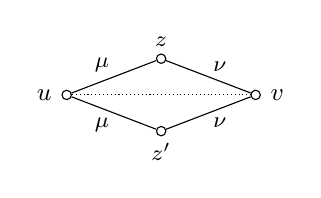
\begin{tikzpicture}[baseline={([yshift=-0.55ex]u.center)},
   every node/.style={font=\footnotesize},vtx/.style={circle,draw,inner sep=1.2pt}]
 \node[vtx,label={[font=\small]left:$u$}] (u) at (0,0) {};
 \node[vtx,label={[font=\small]right:$v$}] (v) at (2.4,0) {};
 \node[vtx,label={[label distance=-1pt]above:$z$}] (z) at (1.2,0.46) {};
 \node[vtx,label={[label distance=-1pt]below:$z'$}] (z2) at (1.2,-0.46) {};
 \draw (u) -- node[above left=-2.5pt] {$\mu$} (z);
 \draw (z) -- node[above right=-2.5pt] {$\nu$} (v);
 \draw (u) -- node[below left=-2.5pt] {$\mu$} (z2);
 \draw (z2) -- node[below right=-2.5pt] {$\nu$} (v);
 \draw[densely dotted] (u) -- (v);
 \end{tikzpicture}
\]
We call such vertices $z$ \defn{witnesses}.
A coloring with this property exists whenever
$|V|\ge n_0(2^k)$, where
$n_0(N)\coloneqq\lceil12N^2\ln(2N)\rceil+3$, since a uniformly random
coloring has it with positive probability
(Lemma~\ref{lem:palette}). These colorings go back to Jipsen, Maddux, and
Tuza~\citep{jipsen-maddux-tuza1995}.

\paragraph{Roadmap.}
In \S\ref{ov:fold}, we construct $2^k$ folds of the reference structure $\mathcal M_0$, each changing the answer of $G_k$ at an unchanged edge.
%
In \S\ref{ov:types}, we show that every circuit gate on $\mathcal M_0$ is constant on each edge-color class and on the diagonal. This allows us to define predictions under each fold.
Boolean operations, including complement, and converse preserve these predictions; only composition can violate them.
%
In \S\ref{ov:twocolors}, we show that, thanks to the two-witness property, each composition can violate the prediction for at most two folds. Since every fold must be detected, any circuit for $G_k$ requires at least $2^{k-1}$ compositions, even with sharing.
\nakamura{violate / detect / notice は重複？（notice は後で定義がある）}

\subsubsection{Folding the reference structure}\label{ov:outline}\label{ov:fold}

We use the reference coloring $\chi$ to define an input structure $\mathcal M_0$ for $G_k$.
On an edge of color $\mu$, we interpret $P_i$ as true exactly when $i\in\mu$, and $Q_i$ exactly when $i\notin\mu$. No input relation holds on loops, which carry the separate label $\id$.
Consequently, a read edge of color $\mu$ accepts exactly witness edges of color $\mu^c$: for distinct $u,v$,
\[
\mathcal M_0 \models G_k(u,v)\iff
\exists z \notin \set{u, v}.\ \chi(u,z)=\chi(u,v)^c.
\]
By the two-witness property, every vertex
has edges of every color, so $G_k$ holds
at every non-loop pair of $\mathcal M_0$.

Fix a vertex $\hub \in V$, the \defn{hub}, and for each color $\mu$ choose $v_\mu$ with $\chi(\hbar,v_\mu)=\mu$.
\nakamura{$\hbar$, $h$, $\hub$ が混在}
%
For each color $\lambda$, let $\chi_\lambda$ be obtained from $\chi$ by recoloring every $\lambda$-colored edge incident to $\hub$ as $\lambda^c$, leaving all other edges unchanged.
Let $\mathcal M_\lambda$ be the input structure induced by $\chi_\lambda$ in the same way as $\mathcal M_0$.
In $\mathcal M_\lambda$, the hub has no edge of color $\lambda$, but the read edge $(\hub,v_{\lambda^c})$ remains unchanged (Figure~\ref{fig:fold}).

\begin{figure}[H]
\begin{minipage}[c]{0.27\linewidth}
\setlength{\abovecaptionskip}{0pt}
\caption[The fold of $\lambda$]{\raggedright The fold of $\lambda$. Only edges at the hub $\hub$ are drawn.}
\label{fig:fold}
\end{minipage}\hfill
\begin{minipage}[c]{0.71\linewidth}
\centering
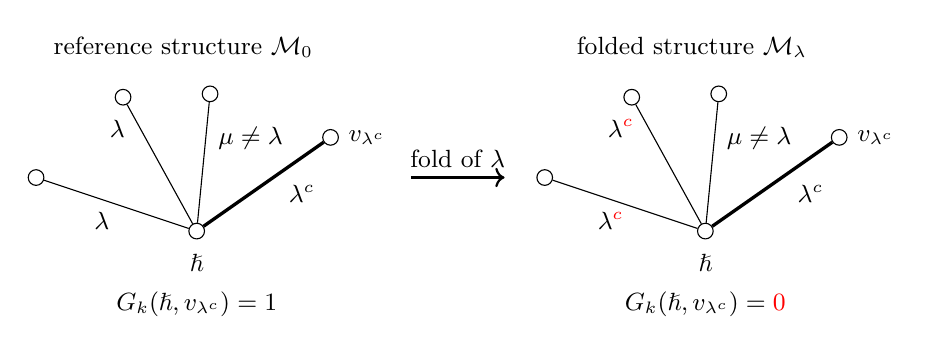
\begin{tikzpicture}[scale=0.85,every node/.style={font=\small},
  vtx/.style={circle,draw,inner sep=2pt}]
\foreach \xs/\col/\val/\name in
  {0/\lambda/1/{reference structure $\mathcal M_0$},
   7.6/\lambda^{\color{red}c}/{\color{red}0}/{folded structure $\mathcal M_\lambda$}}{
\begin{scope}[xshift=\xs cm]
\node at (-0.2,2.75) {\name};
\node[vtx,label={[label distance=2pt]below:$\hub$}] (h) at (0,0) {};
\node[vtx] (a1) at (-2.4,0.8) {};
\node[vtx] (a2) at (-1.1,2.0) {};
\node[vtx] (x) at (0.2,2.05) {};
\node[vtx,label=right:$v_{\lambda^c}$] (v) at (2.0,1.4) {};
\draw (h)--node[below=1pt,pos=0.6] {$\col$} (a1);
\draw (h)--node[left=2pt,pos=0.8] {$\col$} (a2);
\draw (h)--node[right=1pt,pos=0.7] {$\mu\ne\lambda$} (x);
\draw[very thick] (h)--node[below right=0pt,pos=0.62] {$\lambda^c$} (v);
\node at (0,-1.1) {$G_k(\hub,v_{\lambda^c})=\val$};
\end{scope}}
\draw[->,thick] (3.2,0.8)--node[above]{fold of $\lambda$} (4.6,0.8);
\end{tikzpicture}
\end{minipage}
\end{figure}

The read edge $(\hub,v_{\lambda^c})$ requires a $\lambda$-colored edge at $\hub$; the fold removes all such edges. 
\nakamura{辺は削除ではなく、ラベルの反転 (flip)、あるいはラベルの変更か (Fig~\ref{fig:prediction}周辺も同様)}
Hence
\[
\chi_\lambda(\hbar,v_{\lambda^c})
 =\chi(\hbar,v_{\lambda^c})=\lambda^c,\ 
\mathcal M_0\models G_k(\hbar,v_{\lambda^c}),\ 
\mathcal M_\lambda\not\models G_k(\hbar,v_{\lambda^c}).
\]
We call $(\mathcal M_0,\mathcal M_\lambda,(\hub,v_{\lambda^c}))$ the \defn{test} for $\lambda$.
Thus $G_k$ yields $2^k$ tests, one for each color.

\if0
Fix, for each color $\mu$, a vertex $v_\mu$ with $\chi(\hub,v_\mu)=\mu$.
The read edge $(\hub,v_{\lambda^c})$, which the fold of $\lambda$ does not
recolor since $\lambda^c\ne\lambda$, accepts exactly the witness edges of
color $\lambda$. So $G_k(\hub,v_{\lambda^c})$ holds exactly when $\hub$
has an edge of color $\lambda$. Writing $\sem\varphi{\mathcal M}$ also for
the relation that a gate $\varphi$ computes on $\mathcal M$, with value
$\sem\varphi{\mathcal M}(u,v)\in\{0,1\}$ at a pair $(u,v)$, we therefore
get
\[
 \mathcal M_0\xrightarrow{\ \text{fold }\lambda\ }\mathcal M_\lambda
 \quad(\lambda\subseteq[k]),\qquad
 \sem{G_k}{\mathcal M_0}(\hub,v_{\lambda^c})=1\ne0
 =\sem{G_k}{\mathcal M_\lambda}(\hub,v_{\lambda^c}).
\]
We call $\mathcal M_0$, $\mathcal M_\lambda$, and the read edge
$(\hub,v_{\lambda^c})$ the \defn{test} for $\lambda$. So for every color
$\lambda$, every circuit computing $G_k$ has different outputs at the read
edge on $\mathcal M_0$ and on $\mathcal M_\lambda$, although the fold does
not recolor this edge.
\fi


\subsubsection{Circuits see only colors}\label{ov:types}

\paragraph{Color-determined relations.}
A relation $X\subseteq V^2$ is
\defn{color-determined} if
$\chi(u,v)=\chi(u',v') \implies X(u,v)=X(u',v')$ holds.
Here loops carry the separate label $\id$.
Equivalently, $X$ is a union of edge-color
classes, possibly together with the diagonal.
Write $X[\mu]$ for its common value on edges
of color $\mu$, $X[\id]$ for its value on
loops.

Every gate of an arbitrary \CoR\ circuit computes a color-determined relation on $\mathcal M_0$ (Lemma~\ref{lem:tables}).
We can prove this by induction on the
circuit gates. Input relations and constants are
color-determined, while Boolean operations and
converse preserve this property.
The only nontrivial step is composition $X;Y$.

For distinct $u,v$, the two-witness property realizes every pair of colors $\mu,\nu$ along a path $u\xrightarrow{\mu}z\xrightarrow{\nu}v$ with $z\notin\set{u,v}$.
%
The case $z\in\set{u,v}$ depends only on $\chi(u,v)$ and the diagonal values of $X,Y$.
Hence $(X;Y)(u,v)$ depends only on $\chi(u,v)$.
For a loop $(u,u)$, both edges of a path $u-z-u$ have the same color, and every color occurs at every vertex. 
Together with the case $z=u$, this makes $(X;Y)(u,u)$ independent of $u$, completing the induction.


\paragraph{Predicting and noticing a fold.}
A color-determined relation $X$ assigns a value $X[\mu]$ to each color $\mu$.
To predict the effect of a fold, we keep these values fixed and read them at the new edge colors:
\[
\defn{(Prediction)}\quad
X^{(\lambda)}(u,v):=X[\chi_\lambda(u,v)].
\]
Thus a recolored edge reads $X[\lambda^c]$ rather than $X[\lambda]$; all other pairs retain their values.
%
This predicts what a gate would compute if its color-dependent behavior on $\mathcal M_0$ remained unchanged after the fold;
its actual value on $\mathcal M_\lambda$ may differ.

Input relations and constants behave exactly as predicted.
Moreover, Boolean operations and converse commute with prediction
(Proposition~\ref{prop:prediction-commutation}); in particular,
$\overline{X^{(\lambda)}}=(\overline X)^{(\lambda)}$.
Unlike the preservation under embeddings~\eqref{eq:mono} in \S\ref{sec:natural-approaches},
this equality survives unrestricted complement.

Figure~\ref{fig:prediction} compares three operations for any two
distinct colors $\lambda,\mu$: $X$ selects the $\lambda$-colored
edges, and $Y$ the $\mu$-colored edges (both exclude loops).
The thick edge $e=(\hub,v_\mu)$ is unchanged by the fold of
$\lambda$, which removes all $X^{(\lambda)}$-edges at $\hub$.\nakamura{Fig.~\ref{fig:prediction} の表が読めない気がします。列見出しをもう少しちゃんと書くか、caption か本文に説明が欲しいです。
また、Fig.~\ref{fig:prediction} は Fig.~\ref{fig:fold} とほぼ同じにもみえます（あと、塗り替えた辺が Fig.~\ref{fig:prediction} では破線、Fig.~\ref{fig:fold} では実線で、整合性が取れていない）}

\begin{figure}[H]
  \centering
  \begin{minipage}[c]{0.58\linewidth}
    \centering
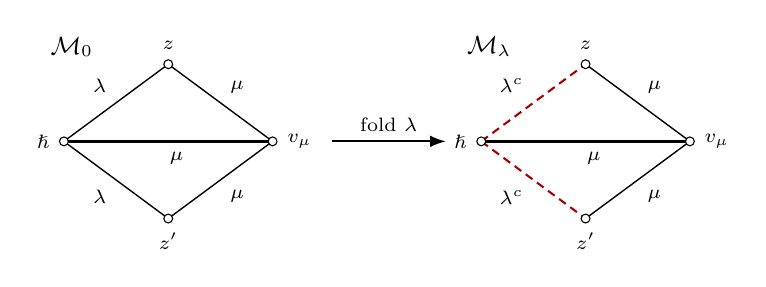
\begin{tikzpicture}[
      >=Latex,
      vertex/.style={circle,draw,fill=white,inner sep=0pt,minimum size=3.2pt},
      edge/.style={line width=.5pt},
      read/.style={line width=1.05pt},
      folded/.style={draw=red!65!black,densely dashed,line width=.75pt},
      every node/.style={font=\scriptsize},
    ]
      % These four vertices show two of the witnesses; the full arena
      % contains further vertices and satisfies the two-witness property.
      \coordinate (h0) at (0,0);
      \coordinate (v0) at (2.65,0);
      \coordinate (z0) at (1.325,0.98);
      \coordinate (w0) at (1.325,-0.98);
      \draw[read] (h0)--node[below,pos=.54] {$\mu$} (v0);
      \draw[edge] (h0)--node[above left] {$\lambda$} (z0);
      \draw[edge] (h0)--node[below left] {$\lambda$} (w0);
      \draw[edge] (z0)--node[above right] {$\mu$} (v0);
      \draw[edge] (w0)--node[below right] {$\mu$} (v0);
      \node[vertex,label=left:{$\hub$}] at (h0) {};
      \node[vertex,label=right:{$v_\mu$}] at (v0) {};
      \node[vertex,label=above:{$z$}] at (z0) {};
      \node[vertex,label=below:{$z'$}] at (w0) {};
      \node[font=\small] at (.1, 1.2) {$\mathcal M_0$};
      \draw[-{Latex[length=2mm]},line width=.7pt]
        (3.4,0)--node[above] {fold $\lambda$} (4.85,0);
      \begin{scope}[xshift=5.30cm]
        \coordinate (h1) at (0,0);
        \coordinate (v1) at (2.65,0);
        \coordinate (z1) at (1.325,0.98);
        \coordinate (w1) at (1.325,-0.98);
        \draw[read] (h1)--node[below,pos=.54] {$\mu$} (v1);
        \draw[folded] (h1)--node[above left,black] {$\lambda^c$} (z1);
        \draw[folded] (h1)--node[below left,black] {$\lambda^c$} (w1);
        \draw[edge] (z1)--node[above right] {$\mu$} (v1);
        \draw[edge] (w1)--node[below right] {$\mu$} (v1);
        \node[vertex,label=left:{$\hub$}] at (h1) {};
        \node[vertex,label=right:{$v_\mu$}] at (v1) {};
        \node[vertex,label=above:{$z$}] at (z1) {};
        \node[vertex,label=below:{$z'$}] at (w1) {};
        \node[font=\small] at (.1, 1.2) {$\mathcal M_\lambda$};
      \end{scope}
    \end{tikzpicture}
  \end{minipage}\hfill%
  \begin{minipage}[c]{0.40\linewidth}
    \centering
    {\footnotesize
    \renewcommand{\arraystretch}{1.16}%
    \begin{tabular}{@{}lccc@{}}
      \toprule
      Operation & Predicted & Actual & Notice? \\
      \midrule
      $X;Y$         & $1$ & $0$ & Yes \\
      $X\cup Y$     & $1$ & $1$ & No \\
      $\overline X$ & $1$ & $1$ & No \\
      \bottomrule
    \end{tabular}}
  \end{minipage}
  \caption{At $e=(\hub,v_\mu)$, only composition notices the fold of $\lambda$.
    Only two witness paths are shown; all $\lambda$-edges at $\hub$ are recolored to $\lambda^c$.}
  \label{fig:prediction}
\end{figure}

\if0
An operation \defn{notices} a fold at given color-determined
operands if applying it after prediction differs from predicting its
result. In Figure~\ref{fig:prediction}, composition notices the fold:
$X^{(\lambda)};Y^{(\lambda)}\ne(X;Y)^{(\lambda)}$.
Union and complement do not notice it; indeed, Proposition~\ref{prop:prediction-commutation}
shows that no Boolean operation or converse can ever notice a fold.
\fi

An operation \defn{notices} a fold at given
color-determined operands if applying it to
their predictions differs from predicting
its result. In Figure~\ref{fig:prediction}, composition notices
the fold at $e$, since
\[
  e\notin\bigl(X^{(\lambda)};Y^{(\lambda)}\bigr)
  \quad \text{and} \quad
  e\in(X;Y)^{(\lambda)}.
\]
By contrast, union and complement do not
notice the fold. More generally, no Boolean
operation or converse can notice any fold
(Proposition~\ref{prop:prediction-commutation}).

Every fold must be noticed by some composition gate.
Let $C$ be a \CoR\ circuit such that $C\equiv G_k$.
If no composition gate notices the fold of $\lambda$,
then, since $(\hub,v_{\lambda^c})$ is unchanged,
Lemma~\ref{lem:unnoticed} gives
\[
  \mathcal M_0\models C(\hub,v_{\lambda^c})
  \quad\Longleftrightarrow\quad
  \mathcal M_\lambda\models C(\hub,v_{\lambda^c}).
\]
This contradicts $C\equiv G_k$, since
$\mathcal M_0\models G_k(\hub,v_{\lambda^c})$
but $\mathcal M_\lambda\not\models G_k(\hub,v_{\lambda^c})$.

\if0
Every fold must be noticed by some composition gate.
Now let $C$ be any circuit computing $G_k$.
If no composition gate notices the fold of
$\lambda$, Lemma~\ref{lem:unnoticed} implies that the output
on $\mathcal M_\lambda$ is the prediction
of the output on $\mathcal M_0$.
Since the test edge $e_\lambda=(\hub,v_{\lambda^c})$ is unchanged,
\[
\sem{C}{\mathcal M_\lambda}(e_\lambda)
=
\bigl(\sem{C}{\mathcal M_0}
\bigr)^{(\lambda)}(e_\lambda)
=
\sem{C}{\mathcal M_0}(e_\lambda),
\]
contradicting the test for $\lambda$, whose outputs are $0$ on $\mathcal M_{\lambda}$ and $1$ on $\mathcal M_0$.
\fi


\subsubsection{Each composition notices at most two folds}\label{ov:twocolors}

We now show that any composition $X;Y$ of color-determined relations
notices at most two folds (Lemma~\ref{lem:local}). The two-witness
property first rules out noticing at pairs away from the hub.

\paragraph{Away from the hub (Figure~\ref{fig:notice}).}
At pairs $(u,v)$ with $u,v\ne\hub$, composition agrees with
prediction.
Figure~\ref{fig:notice} uses the same coloring, operands $X,Y$, and fold
as Figure~\ref{fig:prediction}, but observes $e'=(u,v_\mu)$.

\begin{figure}[H]
  \centering
  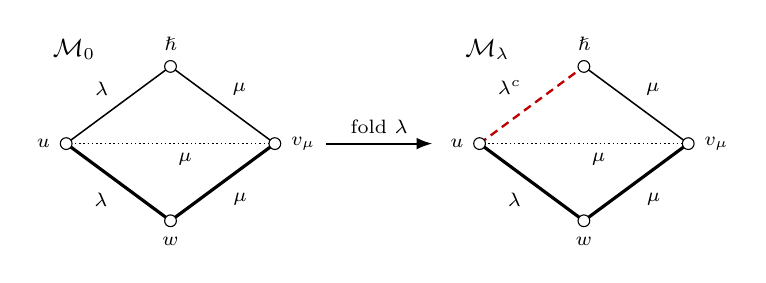
\begin{tikzpicture}[
    >=Latex,
    every node/.style={font=\scriptsize},
    vtx/.style={circle,draw,fill=white,inner sep=1.5pt},
    edge/.style={line width=.55pt},
    recolored/.style={red!75!black,densely dashed,line width=.85pt},
    surviving/.style={line width=1.15pt},
    read/.style={densely dotted,line width=.55pt},
  ]
    % Same four vertices and positions before and after folding.
    % u is the vertex z of Figure 2, and w is its alternative witness.
    \begin{scope}
      \coordinate (u0) at (0,0);
      \coordinate (v0) at (2.65,0);
      \coordinate (h0) at (1.325,.98);
      \coordinate (w0) at (1.325,-.98);
      \draw[read] (u0)--node[below,pos=.57] {$\mu$} (v0);
      \draw[edge] (u0)--node[above left] {$\lambda$} (h0);
      \draw[edge] (h0)--node[above right] {$\mu$} (v0);
      \draw[surviving] (u0)--node[below left] {$\lambda$} (w0);
      \draw[surviving] (w0)--node[below right] {$\mu$} (v0);
      \node[vtx,label=left:{$u$}] at (u0) {};
      \node[vtx,label=right:{$v_\mu$}] at (v0) {};
      \node[vtx,label=above:{$\hub$}] at (h0) {};
      \node[vtx,label=below:{$w$}] at (w0) {};
      \node[font=\small] at (.1, 1.2) {$\mathcal M_0$};
    \end{scope}
    \draw[-{Latex[length=2mm]},line width=.7pt]
      (3.30,0)--node[above] {fold $\lambda$} (4.65,0);
    \begin{scope}[xshift=5.25cm]
      \coordinate (u1) at (0,0);
      \coordinate (v1) at (2.65,0);
      \coordinate (h1) at (1.325,.98);
      \coordinate (w1) at (1.325,-.98);
      \draw[read] (u1)--node[below,pos=.57] {$\mu$} (v1);
      \draw[recolored] (u1)--node[above left,black] {$\lambda^c$} (h1);
      \draw[edge] (h1)--node[above right] {$\mu$} (v1);
      \draw[surviving] (u1)--node[below left] {$\lambda$} (w1);
      \draw[surviving] (w1)--node[below right] {$\mu$} (v1);
      \node[vtx,label=left:{$u$}] at (u1) {};
      \node[vtx,label=right:{$v_\mu$}] at (v1) {};
      \node[vtx,label=above:{$\hub$}] at (h1) {};
      \node[vtx,label=below:{$w$}] at (w1) {};
      \node[font=\small] at (.1, 1.2) {$\mathcal M_\lambda$};
    \end{scope}
  \end{tikzpicture}
  \caption{Away from the hub, the fold invalidates the path through $\hub$
    but leaves the second witness path through $w$ unchanged.
    Only these two witness paths are shown.}
  \label{fig:notice}
\end{figure}

In $\mathcal M_0$, both paths have colors $(\lambda,\mu)$.
After the fold, the path through $\hub$ is invalidated but the path through $w$ survives.
Hence:
$(X^{(\lambda)};Y^{(\lambda)})(e')
=1
=(X;Y)^{(\lambda)}(e')$.

More generally, between any distinct $u,v\ne\hub$, the two-witness
property preserves every two-color path pattern via a witness other
than $\hub$. Loops away from $\hub$ retain edges of every color, and
endpoint witnesses are unchanged. Thus composition cannot violate
prediction away from the hub.

\paragraph{At the hub (Figure~\ref{fig:prediction} revisited).}

Only pairs involving $\hub$ remain.
In Figure~\ref{fig:prediction}, $X$ holds only on $\lambda$ and
$Y$ only on $\mu$, where $\lambda\ne\mu$.
Their composition notices the folds of
$\lambda$ and $\mu$ at $(\hub,v_\mu)$ and
$(v_\lambda,\hub)$, respectively.

Why can it not notice a third fold?
To notice $\lambda$ at $(\hub,v)$, $X$ must
hold on $\lambda$ and no other off-diagonal
color. Indeed, if $X[\nu]=1$ for some
$\nu\ne\lambda$ and $Y[\tau]=1$ for some
color $\tau$, the two-witness property
supplies a path
$\hub\xrightarrow{\nu}z\xrightarrow{\tau}v$
that survives the fold of $\lambda$.
Thus $z$ remains a witness for
$(X^{(\lambda)};Y^{(\lambda)})(\hub,v)$.
%
Likewise, noticing a distinct fold $\mu$
at $(u,\hub)$ requires $Y$ to hold only
on $\mu$. Hence noticing two distinct
folds forces $X$ and $Y$ to be supported
on $\{\lambda\}$ and $\{\mu\}$, respectively.
No third color occurs in either support,
and their supports are disjoint, ruling out
an additional fold noticed at $(\hub,\hub)$.
If $X$ and $Y$ share a color instead,
all possible noticed folds must coincide.
Thus $X;Y$ notices at most two folds.

\paragraph{Summary.}
Every one of the $2^k$ folds requires a noticing composition gate
(\S\ref{ov:types}), whereas each distinct composition gate notices at
most two (Lemma~\ref{lem:local}). Hence $2^k\le 2\gcost C$,
proving the lower bound of Theorem~\ref{thm:main} even with sharing.
% For these tests, the factor two is tight (Proposition~\ref{prop:promise}).



% Requires mathrsfs for \mathscr{P} and TikZ (arrows.meta) for Figure~\ref{fig:reverse-fold}.
\subsection{Further results}\label{sec:additional-results}
In \S\ref{sec:overview}, we explained how folds of a reference structure
prove our main theorem. We now use this approach to establish further
exponential succinctness gaps: from $\FOthree$ to $\FOtwo$, from
$\CoR$ to $\FOtwo$, and from three-attribute relational algebra to
matrix query languages. To explain these extensions, we first summarize
the counting argument of \S\ref{sec:overview}.

Recall that the folds in \S\ref{sec:overview} are indexed by colors $\lambda\in\Lambda=2^{[k]}$.
For a circuit $C \equiv G_k$,
let $D_g\subseteq\Lambda$ be the set of colors whose folds are noticed by gate $g$.
Every color belongs to some $D_g$: otherwise, the circuit
could not detect the change at the read edge left unchanged by that
fold (\S\ref{ov:types}). Thus $\bigcup_{g\in C}D_g=\Lambda$, and
counting gives
\begin{equation}\tag{$\dagger$}\label{eq:fold-counting}
  2^k\le \sum_{g\in C}|D_g|.
\end{equation}
For \CoR, Boolean operations and converse notice no folds, while each
composition notices at most two (\S\ref{ov:twocolors}). Hence
$\sum_{g\in C}|D_g|\le 2\gcost C$, recovering Theorem~\ref{thm:main}.
The applications below use the same counting argument, with different
bounds on the folds noticed by the target operations and, when needed,
a different reference structure.

\paragraph{\texorpdfstring{{\boldmath\FOthree\ to \FOtwo}}{FO3 to FO2}.}
The same query $G_k$ is also \FOtwo-definable: the DNF expansion in
\S\ref{sec:main-results} gives
\[
 G_k(x,y)\equiv\bigvee_{A\subseteq[k]}
 \bigl[H_A(x,y)\land\exists y\,H_{A^c}(x,y)\bigr]
\]
where $H_A$ is \FOtwo-definable.
Here the quantifier binds $y$ only in the second conjunct.
\begin{restatable}[Exponential lower bound from \FOthree\ to \FOtwo\proofref{sec:FOtwo}]{theorem}{sentencebounds}\label{cor:sentences}
For every $k\ge1$,
every \FOtwo\ formula $\varphi$ such that $\varphi\equiv G_k$ has at least $2^k$ quantifiers.

%The bound holds even if $\varphi$ and $G_k$ agree only on finite structures.
\end{restatable}
The displayed expansion uses exactly $2^k$ quantifiers, so the bound
is tight. To our knowledge, this is the first exponential succinctness
gap from \FOthree\ to \FOtwo\ over general finite structures. The gap
also holds for sentences. On pure finite linear orders, by contrast,
\FOthree\ sentences admit polynomial-size \FOtwo\ translations
\citep{grohe-schweikardt2005}, while Vinall-Smeeth's exponential
separations over general structures start at three target variables
\citep{vinall-smeeth2024} (see \S\ref{sec:relwork}).

The same reference structure $\mathcal M_0$ and folds from \S\ref{sec:overview} suffice.
Indeed, regard each \FOtwo\ subformula $\psi$ as a binary relation
$X_\psi$ of assignments to $(x,y)$, with any unused coordinate treated
as a dummy. Quantifying a variable is then a special case of relational
composition:
\[
  X_{\exists y\,\psi}=X_\psi;\one,
  \qquad
  X_{\exists x\,\psi}=\one;X_\psi.
\]
Thus their assignment relations remain color-determined on $\mathcal M_0$,
just like the CoR gate values in \S\ref{sec:overview}.
Since one operand of each composition is $\one$, each quantifier can
notice at most one fold (\S\ref{ov:twocolors}), rather than the two
possible for general composition. Atomic formulas and Boolean
connectives notice none; universal quantifiers are handled by
complement. The counting inequality~\eqref{eq:fold-counting} therefore
requires at least $2^k$ quantifiers. We also obtain a lower bound of $k2^k$ relation-atom occurrences and
optimal tree size $\Theta(k2^k)$, for both queries and sentences
(\S\ref{sec:sentences}).

For \CoR\ itself, we also determine the optimal tree size of $G_k$
as $(2+o(1))k2^k$, whereas its optimal circuit size is $\Theta(2^k)$
(Theorem~\ref{thm:tree}).

\paragraph{\texorpdfstring{{\boldmath\CoR\ to \FOtwo}}{CoR to FO2}.}
An exponential succinctness gap also occurs from \CoR\ to \FOtwo.
We need a different query, since $G_k$ already requires exponentially
many \CoR\ compositions. Put $\mathscr P_i^1\coloneqq\id\cap P_i$
and $\mathscr P_i^0\coloneqq\id\cap\overline{P_i}$, and let
$\vartheta_A(u)\coloneqq\bigwedge_{i\in A}P_i(u,u)\land
\bigwedge_{i\notin A}\neg P_i(u,u)$ for $A\subseteq[k]$.
Consider the following linear-size \CoR\ term and its \FOtwo\ expansion:
\[
\defn{\CoR}:
 U_k \coloneqq R;\bigcap_{i=1}^k
 \left[(\mathscr P_i^0;\one;\mathscr P_i^0)
 \cup(\mathscr P_i^1;\one;\mathscr P_i^1)\right]
 \longrightarrow
\defn{\FOtwo}:
 \bigvee_{A\subseteq[k]}
 \left[\vartheta_A(y)\land\exists y\,
    (R(x,y)\land\vartheta_A(y))\right]
\]
Thus $U_k$ asks whether $x$ has an $R$-successor with the same
$k$-bit loop pattern as $y$.
\begin{restatable}[Exponential lower bound from \CoR\ to \FOtwo\proofref{sec:reverse}]{proposition}{reverse}\label{prop:reverse}
For every $k\ge1$, every \FOtwo\ formula
$\varphi$ such that $\varphi\equiv U_k$ has at least
$2^k$ quantifiers.
% The bound holds even if $\varphi$ and $U_k$ agree only on finite structures.
\end{restatable}

The displayed expansion uses exactly $2^k$ quantifiers, so the bound
is tight.
%
For the lower bound, take a new reference structure $\mathcal W_0$
with several vertices of each loop pattern and a hub $h$ having
$R$-successors of every pattern (Figure~\ref{fig:reverse-fold}).
The fold of $A\subseteq[k]$ deletes all $R$-edges from $h$ to
vertices of pattern $A$.
Thus $U_k(h,y_A)$ changes from true to false
for a vertex $y_A$ of pattern $A$, even when $(h,y_A)$ is unchanged.

\begin{figure}[!htbp]
\centering
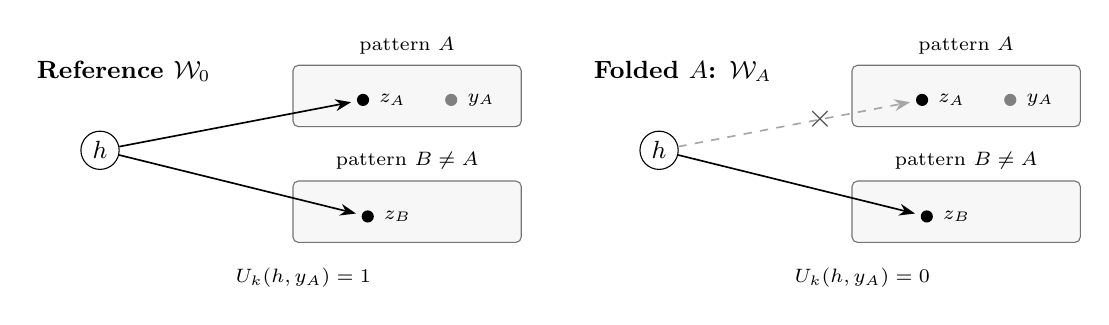
\begin{tikzpicture}[
  >=Stealth,
  every node/.style={font=\small},
  patternclass/.style={draw=black!55, fill=black!3,
      rounded corners=2pt, minimum width=2.9cm, minimum height=.78cm},
  member/.style={circle, fill=black, inner sep=1.55pt},
  testmember/.style={circle, fill=black!50, inner sep=1.55pt},
  redge/.style={->, semithick, shorten >=2pt},
]
\begin{scope}
  \node[font=\bfseries\small] at (0.5, 1.0) {Reference $\mathcal W_0$};
  \node[draw,circle,inner sep=2pt] (h0) at (.20,0) {$h$};
  \node[patternclass] at (4.10,.69) {};
  \node[font=\scriptsize,anchor=south] at (4.10,1.10) {pattern $A$};
  \node[member,label={[font=\scriptsize]right:$z_A$}] (za0) at (3.54,.64) {};
  \node[testmember,label={[font=\scriptsize]right:$y_A$}] at (4.66,.64) {};
  \node[patternclass] at (4.10,-.78) {};
  \node[font=\scriptsize,anchor=south] at (4.10,-.37) {pattern $B\ne A$};
  \node[member,label={[font=\scriptsize]right:$z_B$}] (zb0) at (3.60,-.84) {};
  \draw[redge] (h0) -- (za0);
  \draw[redge] (h0) -- (zb0);
  \node[font=\scriptsize] at (2.78,-1.62) {$U_k(h,y_A)=1$};
\end{scope}
\begin{scope}[xshift=7.1cm]
  \node[font=\bfseries\small] at  (0.5, 1.0) 
  {Folded $A$: $\mathcal W_A$};
  \node[draw,circle,inner sep=2pt] (h1) at (.20,0) {$h$};
  \node[patternclass] at (4.10,.69) {};
  \node[font=\scriptsize,anchor=south] at (4.10,1.10) {pattern $A$};
  \node[member,label={[font=\scriptsize]right:$z_A$}] (za1) at (3.54,.64) {};
  \node[testmember,label={[font=\scriptsize]right:$y_A$}] at (4.66,.64) {};
  \node[patternclass] at (4.10,-.78) {};
  \node[font=\scriptsize,anchor=south] at (4.10,-.37) {pattern $B\ne A$};
  \node[member,label={[font=\scriptsize]right:$z_B$}] (zb1) at (3.60,-.84) {};
  \draw[redge,dashed,black!35] (h1) -- (za1);
  \node[font=\large, text=black!70] at (2.25,.39) {$\times$};
  \draw[redge] (h1) -- (zb1);
  \node[font=\scriptsize] at (2.78,-1.62) {$U_k(h,y_A)=0$};
\end{scope}
\end{tikzpicture}
\caption{The fold of $A$ removes all $R$-edges from $h$ to vertices of loop pattern $A$ (schematic).}
\label{fig:reverse-fold}
\end{figure}

The original folds cannot give this separation: on their reference
structure, every composition notices at most two folds, ruling out a
short \CoR\ term that distinguishes all those tests. In the new
structure, the outer composition of $U_k$ can notice all $2^k$ folds,
whereas each \FOtwo\ quantifier, viewed as a projection, still notices
at most one. The latter bound uses redundant representatives of each
atomic pair type. Applying the same counting argument~\eqref{eq:fold-counting}
to the new tests proves the lower bound (\S\ref{sec:reverse}).

\paragraph{Arity elimination in matrix query languages.}
Brijder~et~al.\ compared two formalisms for semiring-valued queries:
ARA$(3)$, which allows intermediate tables with up to three columns,
and MATLANG, which computes with matrices, vectors, and scalars.
They showed that the two have the same expressive power when inputs
and outputs have at most two columns~\cite{brijder2022}.
Their translation from ARA$(3)$ to MATLANG can grow exponentially,
but whether this blowup is unavoidable was left open~\citep[p.~9]{brijder2019}.
We establish an exponential lower bound using a semiring-valued
analogue of our hard query $G_k$.

Let $\mathfrak S=(S,\oplus,\otimes,0_S,1_S)$ be a commutative semiring,
with input relations $P_i,Q_i:V^2\to S$. Define
\[
  \mathcal G_k(x,y)\coloneqq
  \bigoplus_{z\in V}\ \bigotimes_{i=1}^k
  \Bigl[(P_i(x,y)\otimes Q_i(x,z))
  \oplus(Q_i(x,y)\otimes P_i(x,z))\Bigr].
\]
This query has an ARA$(3)$ expression of size $O(k)$: all $k$
conditions are combined over $(x,y,z)$ before $z$ is aggregated away.
Over Boolean annotations ($S=\mathbb B$, with $\oplus=\lor$ and
$\otimes=\land$), $\mathcal G_k$ specializes to $G_k$.

In MATLANG, the usual semiring matrix--vector (mv) and matrix--matrix
(mm) products take the form
\[
  (A \cdot v)(x) \coloneqq \smash{\bigoplus_{z\in V}} A(x,z)\otimes v(z)
  \quad\text{(mv)},\qquad
  (A \cdot B)(x,y) \coloneqq \smash{\bigoplus_{z\in V}} A(x,z)\otimes B(z,y)
  \quad\text{(mm)}.
\]

Both eliminate their aggregated index immediately.
The DNF of \S\ref{sec:main-results} also gives an explicit MATLANG
representation of $\mathcal G_k$. Here $H_A$ is obtained from the expression in \S\ref{sec:main-results}
by replacing intersections with pointwise $\otimes$, and
$\mathbf 1_S$ is the all-$1_S$ column vector. Then
\[
  \mathcal G_k(x,y)=\smash{\bigoplus_{A\subseteq[k]}}
       H_A(x,y)\otimes (H_{A^c}\mathbf \cdot \mathbf{1}_S)(x).
\]

This uses $2^k$ mv products, together with row broadcasting and
entrywise operations; more general computations may also use mm
products and shared intermediate results.
For a circuit $C$, let $\mvcount C$ count matrix--vector and
vector--matrix aggregations, and $\mmcount C$ count matrix--matrix
aggregations, with shared gates counted once. All other permitted
operations are free.

For a concrete non-Boolean case, consider the natural and integer
min--plus semirings
$\mathsf{Trop}_D \coloneqq (D\cup\{+\infty\},\min,+,+\infty,0)$,
where $D\in\{\mathbb N,\mathbb Z\}$.

\begin{restatable}[Tropical arity-elimination overhead\proofref{sec:matrix}]{theorem}{tropicalmatrixbounds}\label{thm:tropical-matrix}
For every $k\ge1$ and $\mathfrak S\in\{\mathsf{Trop}_{\mathbb N},\mathsf{Trop}_{\mathbb Z}\}$,
the query $\mathcal G_k$ has an ARA$(3)$ expression of size $O(k)$,
but every typed matrix circuit $C$ over $\mathfrak S$ computing it
on all finite inputs satisfies $\mvcount C+3\mmcount C\ge2^k$.
\end{restatable}
The lower bound holds even with arbitrary uniform entrywise functions
and aggregation kernels. Its proof uses the fold-counting principle
\eqref{eq:fold-counting} (\S\ref{sec:matrix}).

The argument extends uniformly beyond tropical matrices.
Examples include the Boolean semiring $(\{0,1\},\lor,\land)$
and the max--min semiring $([0,1],\max,\min)$.
It also covers integer max--plus
$(\mathbb Z\cup\{-\infty\},\max,+)$ and, for each fixed $b\ge1$,
finite-set annotations $(2^{[b]},\cup,\cap)$ and $b$-dimensional
min--plus $\mathsf{Trop}_{\mathbb Z}^{b}$.
One property covers all these examples: \emph{finite join breadth},
meaning that every finite join is determined by a bounded number
of its summands. It bounds how many folds an aggregation can notice,
giving exponential lower bounds for every fixed nontrivial
commutative idempotent semiring of finite join breadth
(Theorem~\ref{cor:matrix}). Over Boolean matrices, we also obtain
the sharper bound $\mvcount C+2\mmcount C\ge2^k$.
Positive computations over nonidempotent semirings such as
$(\mathbb N,+,\times)$ are handled separately by Booleanization
(\S\ref{sec:positive}).

\paragraph{Robustness: closure and randomization.}

The lower bound persists even when \CoR\ is extended with reflexive–transitive closure 
$X^* \coloneqq \bigcup_{m\ge 0}X^m$,
which can be evaluated in $O(n^\omega)$ time~\citep{fischer-meyer1971,munro1971,furman1970}.
Each closure gate notices at most one fold.


\begin{restatable}[Closure does not help\proofref{sec:closure}]{proposition}{closure}\label{prop:star}
Let $C$ be a \CoR\ circuit with closure gates $(-)^*$
and let $g_*(C)$ count its distinct closure gates.
For every $k \ge 1$,
if $C\equiv G_k$, then $2\gcost C+g_*(C)\ge2^k$.
\end{restatable}

The lower bound also extends to bounded-error randomized circuits, even when circuits are specialized to each sufficiently large domain size.

\begin{restatable}[Fixed sizes and bounded error\proofref{sec:query-bounds}]{corollary}{randomizedbounds}\label{cor:randomized}

For some constant $c>0$, for every $k\ge 1$, $n\ge ck4^k$, and $0\le\varepsilon<1/2$, every input-independent distribution of size-specific \CoR\ circuits whose output at each pair $(u,v)$ is correct with probability at least $1-\varepsilon$ on every $n$-element input satisfies
\[
\mathbb E[g_{;}(C)]\ge(1-2\varepsilon)2^{k-1}.
\]
\end{restatable}

\subsection{Related work}\label{sec:relwork}

\paragraph{History of \CoR.}
\CoR\ predates first-order logic as a formal
system. De Morgan introduced relational composition and converse in his
work on the syllogism in the 1850s and 1860s
\citep{demorgan1856,demorgan1864}; Peirce developed the logic of
relatives~\citep{peirce1870,peirce1880}, and Schr\"oder devoted a volume
to it in 1895~\citep{schroeder1895}. This was before first-order logic
was isolated in Hilbert's lectures and Hilbert and Ackermann's
textbook~\citep{hilbert-lectures,hilbert-ackermann1928,moore1988}.
The central expressiveness problem was whether every quantified statement
about relations could be \emph{condensed} into this variable-free calculus.
Schr\"oder claimed that it could~\citep[p.~551]{schroeder1895}, but
Korselt found a counterexample, published by L\"owenheim in
1915~\citep{loewenheim1915,loewenheim1967}. In modern terms, the \FOfour\ sentence
$
\forall a_1\,a_2\,a_3\,a_4.\bigvee_{i,j; i\neq j} a_i = a_j
$
states that the domain has at most three elements, but is expressible
neither in \FOthree\ nor by a \CoR\ equation.

Tarski raised the expressiveness question in 1941~\citep{tarski1941}
and, according to Tarski and Givant, soon obtained the three-variable
characterization: \CoR\ defines exactly the \FOthree-definable binary
queries. A full proof appeared only in their 1987
monograph~\citep{tarski-givant1987}; see
also~\citep{maddux2006}. For historical accounts, see
\citep{pratt1992,maddux1991,burris-legris,brady2000}.
Their original recursive translation~\citep[\S3.9]{tarski-givant1987}
did not analyze its size. A straightforward bottom-up translation using
DNF conversion~\citep{hilbert-ackermann1928,kleene1952,schoening1989}
and quantifier elimination by relational composition gives a
single-exponential upper bound (Appendix~\ref{app:classical-translation});
the reverse \CoR-to-\FOthree\ translation is linear.

\paragraph{Relational computation and quantifier elimination.}
The operations underlying \CoR\ have long served as computational
primitives, often in calculi distinct from full \CoR.
Copilowish gave a matrix-based treatment of the calculus over finite
domains~\citep{copilowish1948}, while Levien and Maron applied relational
operations to retrieval and inference
\citep{levien-maron1965,levien-maron1967,levien1969}.
Codd's relational algebra laid the foundations of database querying
\citep{Codd1970,Codd1972}, followed by work on relational-expression
equivalence, optimization, and efficient join evaluation
\citep{aho-sagiv-ullman1979equiv,aho-sagiv-ullman1979opt,
SelingerEtAl1979,yannakakis1981}.
Binary relational-expression evaluation became an algorithmic subject
\citep{hunt-szymanski-ullman1974,hunt-szymanski-ullman1977,
szymanski-ullman1975,szymanski-ullman1977}, with applications to parsing
and recursive database queries
\citep{sippu-soisalon-soininen1985,grahne-sippu-soisalon-soininen1987,
grahne-sippu-soisalon-soininen1991}.
Related algebras also appear in relational programming, temporal
reasoning, database execution, and graph querying
\citep{maclennan1981,montanari1974,allen1983,boncz-kersten1999,
cruz-mendelzon-wood1987,FletcherEtAl2015,HellingsEtAl2021,
HellingsEtAl2022}.

A second line of work exploits relational composition as existential
quantifier elimination, using matrix multiplication for fast evaluation.
Early examples include transitive closure
\citep{furman1970,fischer-meyer1971,munro1971,oneil-oneil1973,
galil-margalit1993} and algorithms for triangles, cliques, cycles,
and small subgraphs
\citep{itai-rodeh1978,nesetril-poljak1985,alon-yuster-zwick1997,
kloks-kratsch-mueller2000,eisenbrand-grandoni2004,yuster-zwick2004}.
Already in 1977, Chandra and Merlin studied generalized join--project
operations and their evaluation by rectangular Boolean matrix
multiplication~\citep{ChandraMerlin1977}.
Williams's algorithm for prenex first-order graph properties
\citep{Williams2014} can be viewed in the same algebraic framework:
DNF-based quantifier elimination yields ordinary \CoR\ composition
for three quantifiers and typed composition over tuples for larger
prenex formulas, evaluated using rectangular matrix multiplication
(as in \citep{ChandraMerlin1977}).
Gao and Impagliazzo\ \citep{GaoImpagliazzo2019} also treated general
\FOthree\ formulas, beyond prenex normal form, using matrix-based
evaluation.
Related techniques appear in first-order graph algorithms
\citep{BringmannFischerKunnemann2019} and database join--project
and join--aggregate evaluation
\citep{DeepHuKoutris2020,hu-yi2020,Hu2024,AboKhamisHuSuciu2025}.
Most directly, our earlier work used the \FOthree-to-\CoR\ translation
for truly subcubic \FOthree\ model checking
\citep{nakamura-uezato2027}.

\paragraph{Succinctness results.}
Nakamura proved exponential lower bounds for positive \CoR\ and
$\Sigma_1\CoR$, even for circuits, and a superpolynomial separation over
one binary relation~\citep[\S6]{nakamura2022}. The case of full \CoR\
remained open (see \S\ref{sec:natural-approaches}). In our earlier
work~\citep[Corollary~40]{nakamura-uezato2027}, we ruled out
polynomial-time \FOthree-to-\CoR\ translations under the 3-OV
hypothesis, but not the existence of small equivalent representations.
Theorem~\ref{thm:main} gives an unconditional exponential lower bound
even for \CoR\ circuits, while Theorem~\ref{thm:fixed-vocabulary}
gives tight subexponential circuit bounds over one binary relation.

On finite linear orders with no additional relations, Grohe and Schweikardt proved a polynomial-size translation from \FOthree\ to \FOtwo\ sentences~\citep[Theorem~4.3]{grohe-schweikardt2005}. Since \FOtwo\ translates linearly into \CoR, this also yields polynomial-size \CoR\ equations. By contrast, our exponential succinctness gaps from \FOthree\ to both \FOtwo\ and \CoR\ hold even for sentences over general finite structures.
%
They also showed that full first-order logic is exponentially more
succinct than \FOthree\ on the same orders, already witnessed by
\FOfour~\citep[Theorem~5.3]{grohe-schweikardt2005}. The short \FOfour\
formulas combine divide-and-conquer for distances~\citep{savitch1970}
with the classical quantifier-based abbreviation trick, which avoids
duplicating recursive subformulas
\citep{fischer-rabin1974,stockmeyer1974,ferrante-rackoff1979,compton-henson1990,vorobyov1996,stockmeyer-meyer2002}.
The \FOthree\ lower bound draws on Adler--Immerman formula-size
games~\citep{adler-immerman2003}. However, the resulting distance
predicates admit linear-size \CoR\ circuits by repeated squaring,
$S_{i+1}=S_i;S_i$; our lower bound holds even with such sharing.

Vinall-Smeeth established exponential succinctness gaps from
$\mathrm{FO}^{\ell+1}$ to $\mathrm{FO}^{\ell}$ for every $\ell\ge 3$,
using higher-arity (non-binary) relations~\citep[Theorem~2]{vinall-smeeth2024}.
Our result establishes the \FOthree-to-\FOtwo\ case over binary
signatures, with an exponential lower bound on the number of
quantifiers. The linear \FOtwo-to-\CoR\ translation was already
known~\citep{nakamura2022}, while Proposition~\ref{prop:reverse}
gives an exponential gap in the reverse direction.

\paragraph{Lower-bound methods.}
As explained in \S\ref{sec:natural-approaches}, the witness-crossing
argument underlying Nakamura's formula-size-game proof for $\Sigma_1\CoR$
\citep{adler-immerman2003,nakamura2022} relies on embeddings, which fail
under unrestricted complement. We also considered other standard
lower-bound techniques, but their usual resource measures do not directly
fit our setting. Formula-size games
\citep{grohe-schweikardt2005,french2013,hella-vilander2019},
Ehrenfeucht--Fra\"{\i}ss\'e and pebble games
\citep{fraisse1954classif,ehrenfeucht1961,immerman1982,libkin2004},
and multi-structural games
\citep{immerman1981,fagin2021,carmosino2024} address formula size,
quantifier depth, variable count, or quantifier number, rather than the
number of distinct composition gates in circuits with sharing. Indeed,
$G_k$ has only one quantifier and admits a \CoR\ expression of
composition depth one; the issue is the \emph{number} of compositions.
Monotone-circuit lower bounds~\citep{razborov1985,alon-boppana1987}
are natural candidates for our positive query, but equivalent full-\CoR\
circuits may use unrestricted complement. Switching-lemma and
random-restriction methods~\citep{hastad1986} typically exploit
shallow Boolean-circuit structure, whereas we impose no restrictions on
Boolean nesting and charge only compositions.

Communication complexity suggests further approaches. Rank,
discrepancy, and Karchmer--Wigderson techniques
\citep{mehlhorn-schmidt1982,kushilevitz-nisan1997,karchmer-wigderson1990,jukna2012}
do not directly bound compositions when Boolean operations are free.
For example, set disjointness has rank $2^k$, yet its $1$-entries form
the complement of a union of only $k$ rectangles. Alternating existential
and universal witness tests also resemble the nondeterministic and
co-nondeterministic levels of the communication polynomial hierarchy
\citep{babai-frankl-simon1986,goos-pitassi-watson2018}, but we know of
no direct transfer of lower bounds to our circuit model. These approaches did not yield the required composition-count bound.

Our proof instead draws on the affine-plane and random colorings of
Jipsen, Maddux, and Tuza~\citep{jipsen-maddux-tuza1995}, which, as
explained in the technical overview, already yield the two-witness
property needed here. The new ingredient is our fold-based argument:
it bounds how many local folds each distinct operation can notice,
even with unrestricted complement and circuit sharing.

\subsection{Organization}
Section~\ref{sec:aggregation} fixes semantics and resource measures.
Section~\ref{sec:preservation} builds the reference structure, proves
that unnoticed folds leave a circuit's values as predicted and that each
composition notices at most two folds, and states the test--cost
theorem. Section~\ref{sec:logical} supplies the tests for $G_k$ and
proves Theorem~\ref{thm:main} together with the other bounds for
relational circuits: equations, fixed sizes and bounded error, circuits
without converse, domain size, random inputs, and closure.
Section~\ref{sec:fixed-vocabulary} proves the tight fixed-vocabulary
circuit bounds and derives the model-checking application.
Section~\ref{sec:FOtwo} transfers the bound to quantifiers, determines
the minimum term size, and proves Theorem~\ref{cor:sentences} and
Proposition~\ref{prop:reverse}. Section~\ref{sec:matrix} gives a concrete ARA$(3)$ query,
formalizes typed matrix circuits, and extends the fold analysis to
semiring-valued aggregation.
The appendices
give explicit two-witness colorings, the term-size charging argument and
the sharpness of the fold tests, the directed construction for circuits
without converse, and the classical single-exponential translation.



\introproofrefsfalse % restate時にイントロ用のsectionrefを消す


\section{Preliminaries}\label{sec:aggregation}
We fix the semantics of finite-variable formulas, relational terms, and
circuits, with examples that will be used throughout the paper. All
structures have nonempty domains. Our lower bounds concern finite
structures, whereas the explicit translations hold on all nonempty
structures.

\paragraph{Common notation.}

Throughout the paper,
we use $\log x\coloneqq\max\{\log_2 x,1\}$ for $x>0$,
while $\ln$ denotes the natural logarithm.
In running-time bounds, $n^\omega$ is shorthand for $n^{\omega+o(1)}$.

We use $\mathbb N\coloneqq\{0,1,2,\ldots\}$; $\log_2$ is to base two,
and $\ln$ is the natural logarithm. Subscripts on asymptotic notation
indicate the parameters on which hidden constants may depend;
$\operatorname{poly}_\sigma(m)$ also permits the polynomial degree to
depend on $\sigma$.
We use $[k]\coloneqq\{1,\ldots,k\}$ and $2^{[k]}$ for its power set;
$A^c\coloneqq[k]\setminus A$ when $A\subseteq[k]$. Empty intersections and
unions of relations mean $\one$ and $\zero$, respectively; the
analogous Boolean operations mean true and false. Truth values are
$\bool\coloneqq\{0,1\}$, and $[\mathcal P]$ is the indicator of a statement
$\mathcal P$.

\subsection{Finite-variable logic and binary queries}\label{sec:prelim-logic}
\paragraph{Signatures and formulas.}
A \emph{signature} (or \emph{vocabulary}) $\sigma$ is a finite set of binary relation symbols;
there are no function or individual constant symbols. A $\sigma$-structure
$\mathcal M$ has domain $D\coloneqq\operatorname{dom}(\mathcal M)\ne\varnothing$
and interprets each $R\in\sigma$ as a relation $R^{\mathcal M}\subseteq D^2$.
Equality is available. For $\ell\ge1$, the \emph{$\ell$-variable fragment}
$\mathrm{FO}^{\ell}[\sigma]$ consists of first-order formulas using only
$\ell$ variable names, with arbitrary reuse and rebinding of those names.
Formally, with $u,v$ ranging over a fixed set of $\ell$ names, its syntax is
\[
 \varphi::=R(u,v)\mid u=v\mid\neg\varphi
 \mid(\varphi\land\varphi)\mid(\varphi\lor\varphi)
 \mid\exists u\,\varphi\mid\forall u\,\varphi.
\]
We use the names $x,y$ for \FOtwo\ and $x,y,z$ for \FOthree.
The restriction is on the \emph{number of variable names}, not on the
number or nesting depth of quantifiers. For example,
\[
 \varphi(x,y)\coloneqq P(x,y)\land\exists y\,Q(x,y)
\]
is an \FOtwo\ formula: the quantifier rebinds $y$ only in its own scope,
leaving the occurrence of $y$ in $P(x,y)$ free. Write
$\operatorname{FV}(\varphi)$ for the set of free variables.
A \emph{sentence} has no free variables. The \emph{quantifier depth}
is the maximum number of nested quantifiers, not their total number.
We abbreviate $\neg\alpha\lor\gamma$ by $\alpha\to\gamma$, and
$(\alpha\land\gamma)\lor(\neg\alpha\land\neg\gamma)$ by
$\alpha\leftrightarrow\gamma$.
A \emph{positive} formula uses atoms, $\land$, $\lor$, and quantifiers,
but no negation; an \emph{existential-positive} formula also uses no
universal quantifiers. A formula is in \emph{prenex form} if all its
quantifiers precede a quantifier-free formula.

For an assignment $s$ of variables to elements of $D$,
$\mathcal M,s\models\varphi$ means that $\varphi$ is true in
$\mathcal M$ under $s$. For a sentence, its truth is independent of
$s$, and we write $\mathcal M\models\varphi$;
$\mathcal M\not\models\varphi$ means that it is false.

\paragraph{Assignment relations.}
A binary query has an ordered pair of output coordinates, normally
$(x,y)$. For a formula with at most two free variables using other
names, we first fix their correspondence with these coordinates and
apply a consistent permutation of variable names, including bound
occurrences, so that no variable is captured. Under the $(x,y)$ interface, a formula with
$\operatorname{FV}(\varphi)\subseteq\{x,y\}$ defines the
\emph{binary query}
\[
 \sem\varphi{\mathcal M}
 \coloneqq\{(a,b)\in D^2:\mathcal M\models
       \varphi[x\mapsto a,y\mapsto b]\}.
\]
Here $[x\mapsto a,y\mapsto b]$ specifies an assignment, not a
syntactic substitution of individual constants.
A variable absent from $\operatorname{FV}(\varphi)$ contributes a
\emph{dummy coordinate}: the query is independent of its assigned value.
Thus a sentence $\varphi$ has the binary assignment value
\[
 \sem\varphi{\mathcal M}
 =\begin{cases}
     D^2,&\mathcal M\models\varphi,\\
     \varnothing,&\mathcal M\not\models\varphi.
   \end{cases}
\]
This convention lets formulas, relational terms, and circuits have the
same kind of output. An \FOthree\ subformula may nevertheless have
\emph{three} free variables: for example,
$\theta(x,y,z)\coloneqq R(x,z)\land S(z,y)$ has the ternary assignment
relation $\{(a,b,c)\in D^3:R(a,c)\land S(c,b)\}$. Quantifying $z$
returns a binary query. Accordingly, direct \FOthree\ evaluation can
store three-variable truth tables in $O(|\varphi|n^3)$ time on an
$n$-element domain, whereas every intermediate value of a \CoR\ term
or circuit is binary. Section~\ref{sec:matrix} revisits this arity
contrast for matrix query languages.

\subsection{The calculus of relations and relational circuits}\label{sec:prelim-cor}
\paragraph{Relational terms.}
The \emph{calculus of relations} (\CoR) has terms generated by
\[
 T::=R\mid\zero\mid\one\mid\id
   \mid(T\cup T)\mid(T\cap T)\mid\overline T
   \mid T^\smile\mid(T;T), \qquad R\in\sigma.
\]
Write $\sem T{\mathcal M}$ for the binary relation denoted by $T$
on $D$. Its constants are
$\zero\coloneqq\varnothing$, $\one\coloneqq D^2$, and
$\id\coloneqq\{(a,a):a\in D\}$. Union and intersection are set operations;
for relations $X,Y\subseteq D^2$ the other operations are
\[
  \overline X \coloneqq D^2\setminus X,\quad
  X^\smile \coloneqq \set{(b,a):(a,b)\in X},\quad
  (X;Y) \coloneqq 
     \set{ (a, b) : \exists c\in D. (X(a,c)\land Y(c,b)) }.
\]
We identify a relation $X$ with its $\{0,1\}$-valued characteristic
function: $X(a,b)=1$ exactly when $(a,b)\in X$. We also use $X(a,b)$
as this membership predicate, and write $X(e)$ for $X(a,b)$ when
$e=(a,b)$. Complement is unrestricted, including around compositions. A \emph{composition} $X;Y$ is Boolean
matrix multiplication, with $c$ its existential \emph{witness}.

Two useful special cases are the \emph{row and column projections}:
\begin{equation*}\tag{Proj}\label{eq:prelim-projections}
 \begin{aligned}
  (X;\one)(a,b)&\iff\exists c\in D\ X(a,c),\\
  (\one;X)(a,b)&\iff\exists c\in D\ X(c,b).
 \end{aligned}
\end{equation*}
The first is independent of $b$, and the second of $a$. More generally,
for binary predicates $A,B,C$ with the indicated variable pairs,
\begin{equation*}\tag{QE}\label{eq:prelim-elimination}
 \exists z\,\bigl(A(x,y)\land B(x,z)\land C(z,y)\bigr)
 \quad\equiv\quad \bigl(A\cap(B;C)\bigr)(x,y).
\end{equation*}
For example, the \FOtwo\ query
$P(x,y)\land\exists y\,Q(x,y)$ above is $P\cap(Q;\one)$ in \CoR.
The position of complement matters: $\overline{R;\one}$ tests that
$x$ has no $R$-successor, whereas $\overline R;\one$ tests that
$x$ has some non-$R$ pair. These queries are not equivalent.

\paragraph{A linear translation from \FOtwo.}\label{sec:FOtwo-translation}
Under the assignment convention above, the standard translation
$\tau$ from \FOtwo\ into \CoR\ is given on atoms and quantifiers by
\[
\begin{array}{c|c@{\qquad}c|c}
 \varphi&\tau(\varphi)&\varphi&\tau(\varphi)\\\hline
 R(x,y)&R&R(y,x)&R^\smile\\
 R(x,x)&(R\cap\id);\one&R(y,y)&\one;(R\cap\id)\\
 x=y\ \text{or}\ y=x&\id&x=x\ \text{or}\ y=y&\one\\
 \exists x\,\psi&\one;\tau(\psi)&
 \exists y\,\psi&\tau(\psi);\one
\end{array}
\]
Conjunction, disjunction, and negation become intersection, union, and
complement; universal quantifiers use
$\forall u\,\psi\equiv\neg\exists u\,\neg\psi$. Structural induction,
using~\eqref{eq:prelim-projections}, shows that
\[
 \sem{\tau(\varphi)}{\mathcal M}
   =\sem\varphi{\mathcal M},\qquad
 |\tau(\varphi)|=O(|\varphi|).
\]
The translation also preserves the number of relation-atom
occurrences, including reflexive atoms. See
\citep[Remark~3.22]{nakamura2022}. Section~\ref{sec:FOtwo} bounds the fold cost of this translation
by its number of quantifiers.

\paragraph{Terms versus circuits.}
A \emph{term} is a syntax tree, so repeated occurrences of a subterm
are distinct nodes. A \emph{relational circuit} is a finite directed
acyclic graph (DAG): each gate is an input, a constant, or one of the
same \CoR\ operations, with ordered input ports, and a designated
output gate. A gate may feed multiple later gates, including both
ports of one composition. Its value $\sem g{\mathcal M}$ is computed
once from its predecessors; $\sem C{\mathcal M}$ is the value of the
output gate. For any formula, term, or circuit $\Psi$ with a binary
output interface, $\mathcal M\models\Psi(a,b)$ means
$(a,b)\in\sem\Psi{\mathcal M}$, and
$\mathcal M\not\models\Psi(a,b)$ means the opposite.

For example, the term $(R;R);(R;R)$ has seven nodes and three
composition occurrences. The circuit
\[
 g_0\coloneqq R,\qquad g_1\coloneqq g_0;g_0,\qquad g_2\coloneqq g_1;g_1
\]
has just three distinct gates, two of which are compositions
(Figure~\ref{fig:term-vs-circuit}).

\begin{figure}[H]
\centering
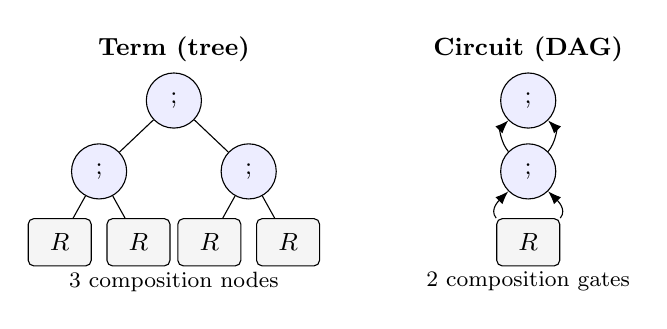
\begin{tikzpicture}[
  comp/.style={draw,circle,fill=blue!7,minimum size=7mm,inner sep=0pt},
  inp/.style={draw,rounded corners=2pt,fill=gray!8,minimum width=8mm,
              minimum height=6mm,inner sep=1pt},
  every node/.style={font=\small},>=Latex]
 \begin{scope}[xshift=-2.25cm]
   \node[font=\small\bfseries] at (0,0.65) {Term (tree)};
   \node[comp] (t0) at (0,0) {$;$};
   \node[comp] (t1) at (-0.95,-0.9) {$;$};
   \node[comp] (t2) at (0.95,-0.9) {$;$};
   \node[inp] (t3) at (-1.45,-1.8) {$R$};
   \node[inp] (t4) at (-0.45,-1.8) {$R$};
   \node[inp] (t5) at (0.45,-1.8) {$R$};
   \node[inp] (t6) at (1.45,-1.8) {$R$};
   \draw (t0)--(t1) (t0)--(t2);
   \draw (t1)--(t3) (t1)--(t4) (t2)--(t5) (t2)--(t6);
   \node[font=\footnotesize] at (0,-2.30) {3 composition nodes};
 \end{scope}
 \begin{scope}[xshift=2.25cm]
   \node[font=\small\bfseries] at (0,0.65) {Circuit (DAG)};
   \node[comp] (c2) at (0,0) {$;$};
   \node[comp] (c1) at (0,-0.9) {$;$};
   \node[inp] (c0) at (0,-1.8) {$R$};
   \draw[-{Latex}] (c0.north west) to[out=130,in=225] (c1.south west);
   \draw[-{Latex}] (c0.north east) to[out=50,in=315] (c1.south east);
   \draw[-{Latex}] (c1.north west) to[out=130,in=225] (c2.south west);
   \draw[-{Latex}] (c1.north east) to[out=50,in=315] (c2.south east);
   \node[font=\footnotesize] at (0,-2.30) {2 composition gates};
 \end{scope}
\end{tikzpicture}
\caption{The term $(R;R);(R;R)$ repeats the same subterm, whereas
 the circuit reuses one gate as both inputs to the next composition.
 Distinct gates, not wires or uses, are counted.}
\label{fig:term-vs-circuit}
\end{figure}

More generally, $g_d$ defined by
$g_{i+1}\coloneqq g_i;g_i$ computes the pairs joined by an $R$-walk of length
$2^d$. Fully unfolding this computation gives a term with $2^d-1$
compositions, while the circuit has only $d$ composition gates.
For another example, a circuit can compute $h\coloneqq R;S$ once and use it
in both branches of $(P\cap h)\cup(Q\cap h^\smile)$, still with only
one composition gate. Thus sharing can save exponentially many
compositions; our lower bounds hold \emph{despite} allowing it.

\paragraph{Equations.}
A \emph{\CoR\ equation} is a statement $T=S$, satisfied by a
structure precisely when
\[
 \mathcal M\models T=S
  \quad\iff\quad
 \sem T{\mathcal M}=\sem S{\mathcal M}.
\]
For example, $\id\cup R=\one$ expresses the \FOtwo\ sentence
$\forall x\,\forall y\,(x=y\lor R(x,y))$. Equivalence between a
\CoR\ equation and an FO sentence means that they hold in exactly
the same structures, rather than that they define the same binary query.
A circuit computing an equation may have two designated output gates
(for $T$ and $S$), with shared intermediate gates counted only once.

\subsection{Resource measures and computational conventions}\label{sec:prelim-resources}
\paragraph{Syntax size and gate counts.}
Formula size $|\varphi|$ and term size $|T|$ count nodes in their
\emph{syntax trees}; all connectives have arity at most two. Negation
and quantification are unary, and displayed iterated connectives are
abbreviations to be expanded, as are $\to$ and $\leftrightarrow$.
Each relation-atom occurrence counts as
one node even for a growing signature (so $|G_k|=8k$); the length of
the written relation name is not charged. This is different from
measuring the encoded bit length of a formula. Write
$\relatoms\varphi$ for the number of relation-atom occurrences
(including $R(x,x)$, but excluding equality atoms), and
$\#_{\exists\forall}(\varphi)$ for its quantifier occurrences.

For a term $T$, write $\relatoms T$ for occurrences of input relation
symbols and $\cost T$ for occurrences of composition. For a circuit
$C$, $|C|$ counts its distinct gates, including input and constant
gates, and $\gcost C$ counts distinct composition gates. All other
operations are uncharged by $\gcost C$, though they do count toward
$|C|$. A shared gate counts once, irrespective of its fan-out. We will
also use the elementary tree inequalities
\[
 |T|\ge2\cost T+1,
 \qquad |T|\ge2\relatoms T-1.
\]

\paragraph{Equivalence and allowed inputs.}
Let $\Psi$ and $\Gamma$ each be a \CoR\ term, a \CoR\ circuit, or
an FO formula with at most two free variables, over a common signature
$\sigma$ and with the same ordered output interface as above. We write
\[
 \Psi\equiv\Gamma
 \quad\iff\quad
 \sem\Psi{\mathcal M}=\sem\Gamma{\mathcal M}
 \quad\text{for every nonempty $\sigma$-structure $\mathcal M$.}
\]
Thus $\equiv$ denotes agreement on arbitrary nonempty structures,
finite or infinite. Our lower bounds are proved using finite test
structures and hold even under the weaker requirement of agreement on
all finite structures. A \emph{size-specific} circuit
$C_n$ may depend on $n=|D|$, but not on the input interpretation;
it must compute the intended query on \emph{every} $n$-element
input. A relational circuit has only the input symbols and the three
constants $\zero,\one,\id$; no built-in order, named vertices,
extra vertex predicates, or arbitrary vertex-dependent constants are
supplied for free. The more permissive typed matrix circuit model of
Section~\ref{sec:typed} is defined separately.

\paragraph{Randomized targets.}
A randomized circuit is an input-independent distribution
$\mathcal D_n$ over deterministic circuits, possibly of different
sizes, for the given domain size $n$. Pointwise error at most
$\varepsilon$ for a query $q$ means that, for every $n$-element input
$\mathcal M$ and every $(a,b)\in D^2$,
\[
 \Pr_{C\sim\mathcal D_n}\!\left[
   \sem C{\mathcal M}(a,b)=\sem q{\mathcal M}(a,b)
 \right]\ge1-\varepsilon.
\]
The entire output relation need not be correct simultaneously.
Randomized resource bounds concern expectations over $\mathcal D_n$;
the circuit distribution is fixed independently of the input.

\section{Folds, predictions, and the test--cost theorem}\label{sec:preservation}
This section proves the machinery of the lower bounds in the order of the
overview. We construct the reference structure (\S\ref{sec:structure}) and
define color-determined relations, folds, and predictions
(\S\ref{sec:types}). We then show
that a relational circuit computes the predicted values on every folded
structure whose fold none of its compositions notices (\S\ref{sec:unnoticed}),
and that each composition notices at most two folds
(\S\ref{sec:responses}). With the tests of \S\ref{sec:G}, this already
proves the composition bounds of Theorem~\ref{thm:main}.
Section~\ref{sec:simultaneous} states the test--cost theorem, a counting
form of the same argument that also covers randomized circuits and the
other targets of \S\ref{sec:additional-results};
Section~\ref{sec:matrix} supplies its hypotheses for scalar-valued
computations.

\subsection{The reference structure}\label{sec:structure}
Fix a palette $\Lambda$ of $N\ge2$ colors and a vertex set $V$ of size $n$.
A coloring $\chi:\binom V2\to\Lambda$ assigns a color to every unordered
pair of distinct vertices. We write $\chi(u,v)$ for $\chi(\{u,v\})$.

\Needspace{7\baselineskip}
\begin{lemma}[Two witnesses]\label{lem:palette}
For every integer
\[
 n\ge n_0(N)\coloneqq\left\lceil12N^2\ln(2N)\right\rceil+3,
\]
there is a coloring such that, for all distinct $u,v\in V$ and all
$\mu,\nu\in\Lambda$, at least two distinct vertices
$z\in V\setminus\{u,v\}$ satisfy
$\chi(u,z)=\mu$ and $\chi(z,v)=\nu$.
\end{lemma}
\begin{proof}
Color the edges independently and uniformly. For fixed distinct $u,v,w$
and colors $\mu,\nu$, the probability that no suitable witness occurs
outside $\{u,v,w\}$ is at most $\exp(-(n-3)/N^2)$: the candidate witnesses
use disjoint pairs of edges. A union bound gives failure probability at most
\[
 n^3N^2\exp(-(n-3)/N^2).
\]
At $n=n_0(N)$, the inequality $n_0(N)\le13N^3$ bounds this expression by
$2197/(4096N)<1$. It decreases for $n>3N^2$, proving the assertion at every
larger size. Hence some coloring has, for all distinct $u,v,w$ and all
colors $\mu,\nu$, a witness outside $\{u,v,w\}$; applying this with $w$
equal to one witness for $u,v$ yields a second.
\end{proof}

Fix such a coloring, and choose a vertex $\hub\in V$, called the
hub. The two witnesses of Lemma~\ref{lem:palette} play different
roles. One witness outside the endpoints already makes every computed
relation a union of color classes, possibly together with the diagonal
(Lemma~\ref{lem:tables}). The second ensures that two vertices other
than $\hub$ have, for every pair of colors, a witness that also avoids
$\hub$, so that recoloring the edges at $\hub$ does not affect pairs away
from it (\S\ref{sec:responses}). Lemma~\ref{lem:palette} also implies that
every vertex sees every color, and that every vertex other than $\hub$
sees every color on edges avoiding $\hub$ (take $v=\hub$). For each color
$\mu$, fix a vertex $v_\mu$ with $\chi(\hub,v_\mu)=\mu$. No vertex,
color, or color neighborhood is supplied as an additional input
predicate.

Jipsen, Maddux, and Tuza~\citep{jipsen-maddux-tuza1995} gave
the random and affine-plane colorings underlying our reference
structures. Although they formulated a one-witness condition, their
constructions also yield the two-witness property used here. The
random-coloring argument above establishes it at every sufficiently
large domain size; their affine-plane coloring has it for planes of
order at least four. Appendix~\ref{app:explicit} verifies the latter
and gives an explicit construction on fewer than $16N^2$ vertices.

\subsection{Color-determined relations, folds, and predictions}\label{sec:types}
For $\mu\in\Lambda$, let
$e_\mu\coloneqq\{(u,v)\in V^2:u\ne v,\ \chi(u,v)=\mu\}$ be the set of edges of
color $\mu$, in both orientations. We extend $\chi$ to loops by giving
every loop the extra label $\diagc$, which is not a color. A relation
$X\subseteq V^2$ is \defn{color-determined} if $X(u,v)$ depends only
on $\chi(u,v)$. For such a relation, write $X[\mu]\in\bool$ for its
common value at pairs $(u,v)$ with $\chi(u,v)=\mu$, where
$\mu\in\Lambda\cup\{\diagc\}$. These $N+1$ values form a table, and
\[
 S_X\coloneqq\{\mu\in\Lambda:X[\mu]=1\}
\]
is the \defn{off-diagonal support} of $X$. Thus $X$ is the union of the
classes $e_\mu$ with $\mu\in S_X$, together with the diagonal if
$X[\diagc]=1$. A reference structure interprets every input relation
by a color-determined relation; we write $\mathcal M_0$ for it.

\begin{lemma}[Closure of color-determined relations]\label{lem:tables}
The constants $\zero,\one,\id$ are color-determined, and
color-determined relations are closed under Boolean operations, converse,
and composition. If $X$ and $Y$ are color-determined, then for every color
$\mu\in\Lambda$,
\begin{equation*}\tag{CT}\label{eq:table-off}
\begin{aligned}
 (X;Y)[\mu]
  &=\bigl(X[\diagc]\land Y[\mu]\bigr)\lor\bigl(X[\mu]\land Y[\diagc]\bigr)
       \lor\bigl(S_X\ne\varnothing\land S_Y\ne\varnothing\bigr),\\
 (X;Y)[\diagc]
  &=\bigl(X[\diagc]\land Y[\diagc]\bigr)\lor\bigl(S_X\cap S_Y\ne\varnothing\bigr),
\end{aligned}
\end{equation*}
where a condition stands for its truth value.
\end{lemma}
\begin{proof}
Boolean operations act entry by entry, and converse preserves this
property because $\chi$ is symmetric. For composition, consider a pair
$(u,v)$ and a potential witness $z$. An endpoint witness,
$z\in\{u,v\}$, contributes the disjuncts of~\eqref{eq:table-off} that involve
$X[\diagc]$ or $Y[\diagc]$. An outside witness, $z\notin\{u,v\}$,
contributes $X[\chi(u,z)]\land Y[\chi(z,v)]$. If $u\ne v$, then by
Lemma~\ref{lem:palette} the color pairs $(\chi(u,z),\chi(z,v))$ of outside
witnesses range over all of $\Lambda\times\Lambda$, so an outside witness
exists exactly when $S_X$ and $S_Y$ are both nonempty. If $u=v$, both
edges of an outside witness are the edge $\{u,z\}$, and every color
occurs on an edge at $u$, so an outside witness exists exactly when
$S_X\cap S_Y\ne\varnothing$.
\end{proof}
In particular, every value of a relational circuit on $\mathcal M_0$ is
color-determined, and
\[
 e_\mu;e_\nu=
 \begin{cases}\one,&\mu=\nu,\\
 \overline{\id},&\mu\ne\nu.
 \end{cases}
\]
Thus the color-determined relations give a concrete representation of
the symmetric relation algebra $E_{N+1}(1,2,3)$ studied by Jipsen,
Maddux, and Tuza~\citep{jipsen-maddux-tuza1995}. Its atoms are $\id$
and the $e_\mu$, and $\overline{\id}=\bigcup_{\mu\in\Lambda}e_\mu$ is
the diversity relation. This identification follows from the displayed
multiplication table, not from automorphisms of the reference graph.

\paragraph{Folds and predictions.}
From now on, take the palette $\Lambda\coloneqq2^{[k]}$ for some $k\ge1$, so that
$N=2^k$. The complement of a color $\mu$ is the color
$\mu^c=[k]\setminus\mu$, and no color equals its complement. The fold of
a color $\lambda$ recolors every edge of color $\lambda$ at the hub to
$\lambda^c$ and leaves all other edges unchanged: for $u\ne v$,
\[
 \chi_\lambda(u,v)\coloneqq
 \begin{cases}\lambda^c,&\hub\in\{u,v\}\text{ and }\chi(u,v)=\lambda,\\
 \chi(u,v),&\text{otherwise},
 \end{cases}
\]
and every loop keeps the label $\diagc$. Only two properties of the fold
matter below: it removes exactly the color $\lambda$ from the hub, and
it changes no edge away from the hub. Any target color other than
$\lambda$ would serve as well. For a color-determined relation $X$,
its prediction $\pred X\lambda$ reads the same values on $\chi_\lambda$:
\[
 \pred X\lambda(u,v)\coloneqq X[\chi_\lambda(u,v)]\qquad(u,v\in V).
\]
Thus $\pred X\lambda$ agrees with $X$ except on the recolored edges,
where it takes the value $X[\lambda^c]$. Replacing every input relation
by its prediction defines the folded structure $\mathcal M_\lambda$ on
the same domain $V$. Predictions are defined only for color-determined relations, in
particular for all values computed on $\mathcal M_0$. We do not assume
that relations computed on $\mathcal M_\lambda$ are color-determined;
in general, they are not.

\subsection{Noticing, and unnoticed folds}\label{sec:unnoticed}
Let $\lambda$ be a color and $\mathbf U=(U_1,\ldots,U_r)$ a tuple of
color-determined relations. For an $r$-ary operation $\operatorname{op}$
such that $\operatorname{op}(\mathbf U)$ is also color-determined, we say
that it notices the fold of $\lambda$ at $\mathbf U$ if
\[
 \operatorname{op}\bigl(\pred{U_1}\lambda,\ldots,\pred{U_r}\lambda\bigr)\ne
 \pred{\operatorname{op}(\mathbf U)}\lambda.
\]
Lemma~\ref{lem:tables} guarantees this condition for the \CoR\ operations.
Both sides are determined by $\mathbf U$ and $\lambda$: noticing is a
property of the operands on $\mathcal M_0$, not of any computation on
$\mathcal M_\lambda$.

\begin{proposition}[Commutation with prediction]\label{prop:prediction-commutation}
For any color $\lambda$ and color-determined relations $X,Y$, prediction
commutes with Boolean operations and converse:
\[
\begin{aligned}
 \pred{(X\cup Y)}\lambda&=\pred X\lambda\cup\pred Y\lambda,&
 \pred{(X\cap Y)}\lambda&=\pred X\lambda\cap\pred Y\lambda,\\
 \pred{(\overline X)}\lambda&=\overline{\pred X\lambda},&
 \pred{(X^\smile)}\lambda&=(\pred X\lambda)^\smile.
\end{aligned}
\]
The constants $\zero,\one,\id$ are also fixed by prediction.
\end{proposition}
\begin{proof}
Boolean operations act pair by pair, so both sides apply the same
operation to the entries at $\chi_\lambda(u,v)$. Converse commutes with
prediction because $\chi_\lambda(u,v)=\chi_\lambda(v,u)$. The constants
are fixed because a fold preserves the diagonal.
\end{proof}

Thus only composition can notice a fold. A composition gate of a
relational circuit notices the fold of $\lambda$ if the composition of
its operand values on $\mathcal M_0$ notices it.
\begin{lemma}[Unnoticed folds]\label{lem:unnoticed}
Let $C$ be a relational circuit and $\lambda$ a color. If no composition
gate of $C$ notices the fold of $\lambda$, then on $\mathcal M_\lambda$
every gate of $C$ computes the prediction of its value on $\mathcal M_0$.
In particular, the outputs of $C$ on $\mathcal M_0$ and on
$\mathcal M_\lambda$ agree at every pair that the fold does not recolor.
\end{lemma}
\begin{proof}
Evaluate $C$ on $\mathcal M_0$. By Lemma~\ref{lem:tables}, every gate
value is color-determined, so its prediction is defined. We show by
induction along a topological order of the gates that every gate computes
on $\mathcal M_\lambda$ the prediction of its value on $\mathcal M_0$. For
input relations this is the definition of $\mathcal M_\lambda$, and
constants are their own predictions by Proposition~\ref{prop:prediction-commutation}.
For Boolean and converse gates, the claim follows from the induction
hypothesis and Proposition~\ref{prop:prediction-commutation}.
If the operands of a composition gate have values $X$ and $Y$ on
$\mathcal M_0$, then by induction they have values $\pred X\lambda$ and $\pred Y\lambda$ on
$\mathcal M_\lambda$. The gate therefore computes
$\pred X\lambda;\pred Y\lambda$ on $\mathcal M_\lambda$, which equals
$\pred{(X;Y)}\lambda$ because the gate does not notice the fold. Finally,
every value $U$ on $\mathcal M_0$ agrees with $\pred U\lambda$ at every
pair that the fold does not recolor.
\end{proof}

\subsection{Each composition notices at most two folds}\label{sec:responses}
Fix color-determined relations $X,Y$ and a color $\lambda$, and write
$J\coloneqq\Lambda\setminus\{\lambda\}$ for the set of colors at $\hub$
after the fold of $\lambda$.
Endpoint witnesses contribute the same value to
$\pred X\lambda;\pred Y\lambda$ and to $\pred{(X;Y)}\lambda$. At a pair
$(u,v)$ with $u\ne v$ and $\mu\coloneqq\chi_\lambda(u,v)$, they contribute
$(X[\diagc]\land Y[\mu])\lor(X[\mu]\land Y[\diagc])$ to
$\pred X\lambda;\pred Y\lambda$, because $\pred X\lambda$ and
$\pred Y\lambda$ take the values $X[\diagc]$ and $Y[\diagc]$ on the
diagonal and $X[\mu]$ and $Y[\mu]$ at $(u,v)$, and the same value to
$\pred{(X;Y)}\lambda(u,v)=(X;Y)[\mu]$ by~\eqref{eq:table-off}; at a
diagonal pair, they contribute $X[\diagc]\land Y[\diagc]$ to both. The
following table compares the outside witnesses. Its left column states
when $\pred X\lambda;\pred Y\lambda$ has an outside witness at the pair,
and its right column states the last disjunct of~\eqref{eq:table-off},
which $\pred{(X;Y)}\lambda$ reads at the pair; here $u$ and $v$ range
over vertices other than $\hub$, and $S\ne\varnothing\ne S'$ means that
both sets are nonempty.
\begin{center}
\renewcommand{\arraystretch}{1.15}
\begin{tabular}{lll}
\toprule
Output pair & Outside witness in $\pred X\lambda;\pred Y\lambda$
 & Last disjunct of~\eqref{eq:table-off}\\
\midrule
$(u,v)$, $u\ne v$ & $S_X\ne\varnothing\ne S_Y$ & $S_X\ne\varnothing\ne S_Y$\\
$(u,u)$ & $S_X\cap S_Y\ne\varnothing$ & $S_X\cap S_Y\ne\varnothing$\\
$(\hub,v)$ & $S_X\cap J\ne\varnothing\ne S_Y$ & $S_X\ne\varnothing\ne S_Y$\\
$(u,\hub)$ & $S_X\ne\varnothing\ne S_Y\cap J$ & $S_X\ne\varnothing\ne S_Y$\\
$(\hub,\hub)$ & $S_X\cap S_Y\cap J\ne\varnothing$ & $S_X\cap S_Y\ne\varnothing$\\
\bottomrule
\end{tabular}
\end{center}
For the left column, consider the outside witnesses $z$ of a pair. For
distinct $u,v\ne\hub$, Lemma~\ref{lem:palette} gives, for every pair of
colors, an outside witness other than $\hub$, whose two edges keep their
colors; the witness $\hub$ contributes one more color pair, which is
already realized. For $(u,u)$ with $u\ne\hub$, every color occurs on an
edge at $u$ that avoids $\hub$. At a pair $(\hub,v)$ of the
\defn{hub row}, the left edge $\{\hub,z\}$ of every outside witness lies
at the hub, so its color becomes $\chi_\lambda(\hub,z)\in J$, while the
right edge $\{z,v\}$ keeps its color; by Lemma~\ref{lem:palette} the
realized color pairs are exactly $J\times\Lambda$. The pairs $(u,\hub)$
of the \defn{hub column} are symmetric, with $\Lambda\times J$. At
$(\hub,\hub)$ both edges of an outside witness are the edge
$\{\hub,z\}$, whose color $\chi_\lambda(\hub,z)$ ranges exactly over $J$.

\begin{lemma}[When a composition notices a fold]\label{lem:local}\label{lem:notice}
Let $X,Y$ be color-determined. The composition $X;Y$
notices the fold of $\lambda$ only if
\[
 S_X=\{\lambda\},\qquad S_Y=\{\lambda\},\qquad\text{or}\qquad
 S_X\cap S_Y=\{\lambda\}.
\]
Hence it notices at most two folds, at most one if $S_X$ or $S_Y$ is
$\varnothing$ or $\Lambda$, and none if both are.
\end{lemma}
\begin{proof}
By the table, the two sides can differ only in the hub row, in the hub
column, or at $(\hub,\hub)$. In the hub row they can differ only if
$S_X\ne\varnothing$ but $S_X\cap J=\varnothing$, that is,
$S_X=\{\lambda\}$; in the hub column only if $S_Y=\{\lambda\}$; and at
$(\hub,\hub)$ only if $S_X\cap S_Y=\{\lambda\}$. Each condition
determines $\lambda$. If $S_X\cap S_Y\ne\varnothing$, each of the first
two conditions implies the third, so at most one fold is noticed;
otherwise the third condition never holds, and at most two are. If $S_Y$
is $\varnothing$ or $\Lambda$, then $S_Y\ne\{\lambda\}$ because $N\ge2$,
and $S_X\cap S_Y$ is $\varnothing$ or $S_X$, so only the condition
$S_X=\{\lambda\}$ remains; the case of $S_X$ is symmetric. If both are
$\varnothing$ or $\Lambda$, none of the conditions can hold.
\end{proof}
The bound two is attained. The composition $e_\mu;e_{\mu^c}$ has
$S_X=\{\mu\}$ and $S_Y=\{\mu^c\}$, and notices the folds of both $\mu$
and $\mu^c$. On the reference structure of \S\ref{sec:G}, the relation
$e_\mu$ is the relation $H_\mu$ of the DNF.
Proposition~\ref{prop:promise} computes $G_k$ on the reference structure
and all its folded structures with $2^{k-1}$ such compositions.
By Lemma~\ref{lem:notice}, each composition gate notices at most two
folds. What a gate notices depends only on its operand values on
$\mathcal M_0$, so a shared gate counts once, regardless of its fan-out.
Hence at most $2\gcost C$ folds are noticed by some gate of $C$, and
Lemma~\ref{lem:unnoticed} applies to all other folds. Nothing here
depends on the query or on the interpretation of the input relations. If
a query has different answers on $\mathcal M_0$ and on
$\mathcal M_\lambda$ at a pair that the fold of $\lambda$ does not
recolor, for every color $\lambda$, then every relational circuit $C$
defining it satisfies $2\gcost C\ge2^k$. Section~\ref{sec:logical} shows
that $G_k$ is such a query.

\subsection{Tests and the test--cost theorem}\label{sec:simultaneous}
For randomized circuits and for the other targets of
\S\ref{sec:additional-results}, we formalize the same
\emph{fold-counting argument} as a test--cost theorem, using only a few
abstract properties. For a color $\lambda$,
the \defn{test} for $\lambda$ consists of the structures $\mathcal M_0$
and $\mathcal M_\lambda$ and the \defn{output observation}
$\rho_\lambda(U)\coloneqq U(\hub,v_{\lambda^c})$, the entry of an output
value $U$ at the pair $(\hub,v_{\lambda^c})$ of \S\ref{sec:structure}.
Since $\lambda^c\ne\lambda$, the fold of $\lambda$ does not recolor this
pair, so
\begin{equation*}\tag{O}\label{eq:observation}
 \rho_\lambda(\pred U\lambda)=\rho_\lambda(U)
\end{equation*}
for every reference output value $U$, as defined in~(i) below.

The counting argument uses only three properties of this construction.
We call data satisfying them a \defn{test system}:
\begin{enumerate}[label=(\roman*),leftmargin=*]
\item Each type of value has a collection of \defn{reference values},
which contains the input values on $\mathcal M_0$ and is closed under the
permitted operations, and every reference value $U$ has a prediction
$\pred U\lambda$ for each color $\lambda$.
\item Every input value on $\mathcal M_\lambda$ is the prediction of the
same input value on $\mathcal M_0$.
\item Every test satisfies~\eqref{eq:observation}, and the required
answers at its observation on $\mathcal M_0$ and on $\mathcal M_\lambda$
differ.
\end{enumerate}
For relational circuits, the reference values are the color-determined
relations, and Lemma~\ref{lem:tables} supplies~(i). The typed scalar
computations in \S\ref{sec:matrix} will satisfy the same conditions;
predictions carry the type of their argument, which we suppress in the
notation. For a gate $g$ of a deterministic circuit $C$, let
$\operatorname{op}_g$ be its operation and $\mathbf U_g$ the tuple of its
operand values on $\mathcal M_0$. As in \S\ref{sec:unnoticed}, $g$
notices the fold of $\lambda$ if
$\operatorname{op}_g(\pred{\mathbf U_g}\lambda)\ne
\pred{\operatorname{op}_g(\mathbf U_g)}\lambda$, where predictions act
componentwise on tuples. Define
\[
 \begin{split}
 D_g&\coloneqq\{\lambda\in\Lambda:g\text{ notices the fold of }\lambda\},\\
 \tcost(C)&\coloneqq\sum_{g\text{ distinct}}|D_g|.
 \end{split}
\]
For input nodes put $D_g\coloneqq\varnothing$; constant gates are nullary
operations. The definition of $D_g$ compares the entire output of the
gate, and it uses predicted operands computed from $\mathcal M_0$, not
operands recomputed on $\mathcal M_\lambda$.

We call $\tcost(C)$ the \defn{cost} of $C$. It counts the pairs of a
distinct gate and a fold that the gate notices. This integer depends on
the reference structure and the tests, which remain fixed, but is
defined even for an incorrect circuit.

\begin{theorem}[Test--cost theorem]\label{thm:test-cost}
Fix a test system. A deterministic circuit $C$ correct at both
observations of every test satisfies
\[
 2^k\le\tcost(C).
\]
If $C$ is drawn from an input-independent distribution $\mathcal D$ of
circuits, and each observation in each test is incorrect with probability
at most $\varepsilon<1/2$, then
\[
 (1-2\varepsilon)2^k\le
 \mathbb E_{C\sim\mathcal D}[\tcost(C)].
\]
\end{theorem}
\begin{proof}
Fix a deterministic circuit, not assumed correct, and put
$D_C\coloneqq\bigcup_gD_g$. For $\lambda\notin D_C$, no gate notices the
fold of $\lambda$, so the induction in the proof of
Lemma~\ref{lem:unnoticed}, with~(ii) for the input values, gives
\[
 \sem C{\mathcal M_\lambda}=\pred{(\sem C{\mathcal M_0})}\lambda.
\]
The equality concerns the whole output. By the observation
condition~\eqref{eq:observation}, the two observations are equal, whereas
their correct values differ. Hence at least one is wrong. If
$\mathrm{err}_{\lambda,0}(C),\mathrm{err}_{\lambda,1}(C)$ are the
corresponding zero-one error indicators, then
\[
 \tcost(C)+\sum_{\lambda\in\Lambda}
   \bigl(\mathrm{err}_{\lambda,0}(C)+\mathrm{err}_{\lambda,1}(C)\bigr)\ge2^k,
\]
because $|D_C|\le\tcost(C)$. Zero error proves the first assertion.
Take expectations using the same random circuit on the two structures
of each test. Each error indicator has expectation at most $\varepsilon$,
which proves the second assertion. No independence among the tests or
their errors is required.
\end{proof}

For lower bounds obtained from the color-based reference structures
of \S\ref{sec:structure}, this argument also gives fixed-size and
randomized forms. Each such bound estimates $\tcost(C)$ from above by
a resource count, such as $2\gcost C$ in Lemma~\ref{lem:cor-cost}. First, Lemma~\ref{lem:palette} gives the
reference structure on every domain of size $n\ge n_0(2^k)$, and the
folds keep the domain, so each bound holds for targets that need to be
correct only on $n$-element inputs and may be chosen for $n$. Second, by
the randomized assertion of Theorem~\ref{thm:test-cost}, each bound for
targets that compute a query also holds for an input-independent
distribution of targets with pointwise error at most
$\varepsilon<1/2$, after the resource count is replaced by its
expectation and the bound is multiplied by $1-2\varepsilon$; for scalar
outputs, an error is a failure to return the exact required value.

For ordinary \CoR, call a composition gate whose operand values on
$\mathcal M_0$ are $X,Y$ \defn{one-sided} if $S_X$ or $S_Y$ is
$\varnothing$ or $\Lambda$. Let
$m_1(C)$ count these gates and $m_2(C)$ the other composition gates,
counting shared gates once.
\begin{lemma}[Cost of compositions]\label{lem:cor-cost}
Every relational circuit $C$ satisfies
\[
 \tcost(C)\le m_1(C)+2m_2(C)\le2\gcost{C}.
\]
\end{lemma}
\begin{proof}
By Lemma~\ref{lem:local}, a one-sided composition notices at most one
fold and any other composition at most two. Other gates notice nothing.
Summing over distinct gates proves the inequalities.
\end{proof}
The row and column projections $X;\one$ and $\one;X$ of
\S\ref{sec:prelim-cor} are examples of one-sided compositions; the
one-sided condition itself is semantic and may hold for other gates.
If a syntactic count is preferred, one may charge all non-projection
compositions at cost two, without changing Lemma~\ref{lem:cor-cost}.

\section{Lower bounds for relational circuits}\label{sec:logical}
The construction of \S\ref{sec:preservation} is independent of the
query. We now interpret the input relations of $G_k$ on it; the read
edge of each test identifies the witness color that the fold removes.

\subsection{The tests for \texorpdfstring{$G_k$}{Gk}}\label{sec:G}
On a color $\mu$, interpret $P_i$ as $1$ precisely when $i\in\mu$, and
$Q_i$ as $1$ precisely when $i\notin\mu$. Put both values zero on every
loop. More explicitly,
\[
 P_i^{\mathcal M_0}\coloneqq\bigcup_{\mu\in\Lambda:\,i\in\mu}e_\mu,\qquad
 Q_i^{\mathcal M_0}\coloneqq\bigcup_{\mu\in\Lambda:\,i\notin\mu}e_\mu.
\]
For each color $\lambda$, use the read edge $(\hub,v_{\lambda^c})$,
of color $\lambda^c$ (\S\ref{sec:structure}), and the fold of $\lambda$
(\S\ref{sec:types}). Since $\lambda\ne\lambda^c$, the fold does not
recolor this read edge.

\begin{lemma}[The tests for $G_k$]\label{lem:G-tests}
For every color $\lambda$,
\[
 \sem{G_k}{\mathcal M_0}(\hub,v_{\lambda^c})=1,\qquad
 \sem{G_k}{\mathcal M_\lambda}(\hub,v_{\lambda^c})=0.
\]
Moreover, the sentence $G_k^\forall=\forall x\,\forall y\,(x=y\lor
G_k(x,y))$ of \S\ref{sec:main-results} is true in $\mathcal M_0$
and false in every $\mathcal M_\lambda$. Thus $G_k$ and $G_k^\forall$
each supply $2^k$ tests.
\end{lemma}
\begin{proof}
For non-loop edges with colors $\mu,\nu$, the body of $G_k$ holds
exactly when $\nu=\mu^c$. A loop, whose $P_i,Q_i$ values are all zero,
cannot be a witness edge. Hence, on $\mathcal M_0$ and on every
$\mathcal M_\lambda$, $G_k$ holds at a pair $(u,v)$ of distinct vertices
exactly when $u$ has an edge whose color is the complement of the color
of $(u,v)$. Against the read color $\lambda^c$, the sole accepted
witness color is $\lambda$. That color occurs at $\hub$ in
$\mathcal M_0$ and does not occur there after the fold. In
$\mathcal M_0$, every vertex has edges of every color, so $G_k$ holds at
every pair of distinct vertices, and $x=y$ handles the diagonal; in
$\mathcal M_\lambda$, $G_k$ fails at the pair $(\hub,v_{\lambda^c})$ of
distinct vertices.
\end{proof}

\subsection{Consequences}\label{sec:query-bounds}
\mainbounds*
\begin{proof}
Let $C\equiv G_k$, or more generally let $C$ agree with $G_k$
on all finite structures. Take the reference structure at any size
$n\ge n_0(2^k)$. For each color $\lambda$, the answers of $G_k$
at $(\hub,v_{\lambda^c})$ on $\mathcal M_0$ and on $\mathcal M_\lambda$ differ
by Lemma~\ref{lem:G-tests}, and the fold of $\lambda$ does not recolor
this pair. By Lemma~\ref{lem:unnoticed}, some composition gate of $C$
notices the fold of $\lambda$. By Lemma~\ref{lem:notice}, each
composition gate notices at most two folds, so $2\gcost C\ge2^k$. A term
is a circuit without sharing, so the same bound holds for its number of
compositions.
\end{proof}
Together with the expansion of $G_k$ in \S\ref{sec:main-results}, these
lower bounds show that the minimum circuit size for $G_k$ is
$\Theta(2^k)$; Theorem~\ref{thm:tree} in \S\ref{sec:trees}
determines the minimum term size.

The lower bound does not rest on the difficulty of evaluating $G_k$. As
its proof shows, it holds even for circuits that are correct only on the
reference structure and its folded structures, on which every non-loop
edge has a color from the palette. A read edge there accepts exactly the
witness edges of the complementary color, so a trie of the colors
present in each row evaluates $G_k$ on all pairs of these structures in
time $O(kn^2)$, linear in the size of the input.

\paragraph{Equations.}
By the semantics of \CoR\ equations in \S\ref{sec:prelim-cor},
the same tests also bound the equational form of Tarski's correspondence.
\begin{corollary}[\CoR\ equations]\label{cor:equations}
If a \CoR\ equation $T=S$ holds on exactly those finite structures that
satisfy $G_k^\forall$, then every relational circuit with gates computing
$T$ and $S$ has at least $2^{k-1}-1$ composition gates.
\end{corollary}
\begin{proof}
Let $C$ have gates computing $T$ and $S$, and add gates for
\[
 \mathrm{Eq}\coloneqq\overline{\one;\bigl((T\cap\overline S)\cup(\overline T\cap S)\bigr);\one},
\]
which is the full relation when $T=S$ and empty otherwise. This adds two
compositions, both one-sided. By Lemma~\ref{lem:G-tests}, $G_k^\forall$
is true in $\mathcal M_0$ and false in every $\mathcal M_\lambda$, so
$\mathrm{Eq}$ is full on $\mathcal M_0$ and empty on every
$\mathcal M_\lambda$. Both constants are their own predictions, so these
are $2^k$ tests, and Theorem~\ref{thm:test-cost} with
Lemma~\ref{lem:cor-cost} gives $2^k\le2\gcost C+2$.
\end{proof}
The DNF of \S\ref{sec:main-results} gives the equivalent equation
$\id\cup\bigcup_{A\subseteq[k]}[H_A\cap(H_{A^c};\one)]=\one$
with $2^k$ compositions, so the bound is tight up to a factor of two.

\paragraph{Fixed sizes and bounded error.}
The reference structure and its folded structures share one domain,
which may have any size $n\ge n_0(2^k)$, and the randomized assertion of
Theorem~\ref{thm:test-cost} handles bounded error.
\randomizedbounds*
\begin{proof}
At the prescribed size $n$, Lemma~\ref{lem:palette} gives the reference
structure, and Lemma~\ref{lem:G-tests} gives all $2^k$ tests on that domain.
Apply the expected-cost assertion of Theorem~\ref{thm:test-cost} and
$\tcost(C)\le2\gcost C$. Setting $\varepsilon=0$ includes every exact
size-specific circuit.
\end{proof}

\paragraph{Circuits without converse.}
Without converse, a directed version of the reference structure lets
each composition notice at most one fold, and the bound becomes exact.
\begin{restatable}[Without converse]{corollary}{withoutconverse}\label{cor:without-converse}
For every $k\ge1$, every relational circuit without converse that
defines $G_k$ on finite structures has at least $2^k$ composition gates.
This bound is attained by the DNF.
\end{restatable}
Appendix~\ref{app:directed} proves the corollary with a directed
reference coloring. For full \CoR, Proposition~\ref{prop:promise} gives
a circuit with $2^{k-1}$ compositions that is correct on the reference
structure and all its folded structures. Thus these tests attain the
coefficient two of Lemma~\ref{lem:notice} and cannot give more than
$2^{k-1}$. The optimum for $G_k$ on arbitrary inputs remains between
$2^{k-1}$ and $2^k$.

\subsection{Domain size}\label{sec:domain-size}
On arbitrary inputs, the \defn{pair profile} is the ordered bit vector
\[
 \pi(x,z)\coloneqq
 ([P_1(x,z)],\ldots,[P_k(x,z)],
  [Q_1(x,z)],\ldots,[Q_k(x,z)])\in\{0,1\}^{2k}.
\]
On the reference structure, the profile of an edge is determined by its color.
By the definition of $G_k$,
the read edge $(x,y)$ accepts the witness edge $(x,z)$ exactly when, for
every $i$, the profile $\pi(x,y)$ has $P_i$ and $\pi(x,z)$ has $Q_i$, or
$\pi(x,y)$ has $Q_i$ and $\pi(x,z)$ has $P_i$. Hence $G_k(x,y)$ depends
only on $\pi(x,y)$ and the set $\Pi_x\coloneqq\{\pi(x,z):z\in V\}$ of profiles in
row $x$, which has at most $|V|$ elements.

\begin{proposition}[Small domains]\label{prop:small-domains}
For all $k,n\ge1$ there is a converse-free relational circuit with $4kn$
composition gates, all of them row projections $X;\one$, and $O(k^2n^2)$
other gates, that computes $G_k$ on every structure with at most $n$
elements.
\end{proposition}
\begin{proof}
A relation is \defn{row-constant} if its value at $(x,y)$ does not
depend on $y$. By~\eqref{eq:prelim-projections}, each row projection $S;\one$
is row-constant and holds in row $x$ exactly when some pair
$(x,z)$ lies in $S$; Boolean
combinations of row-constant relations are row-constant. For
$1\le b\le2k$, let $E_b$ be the input relation giving bit $b$ of the
profile, and put $E_b^1\coloneqq E_b$ and $E_b^0\coloneqq\overline{E_b}$.

In a structure with at most $n$ elements, call a word
$w\in\{0,1\}^\ell$ \defn{live} in row $x$ if some profile in $\Pi_x$
begins with $w$. Live words of one length begin distinct profiles, so
there are at most $n$ of each length, and the empty word is live because
$\pi(x,x)\in\Pi_x$. The circuit stores the live words of length $\ell$ in
$n$ slots: row-constant relations $L_{\ell,r}$ and $W_{\ell,r,b}$, for
$1\le r\le n$ and $1\le b\le\ell$, state that slot $r$ is occupied in row $x$ and
that its word has bit $b$. The invariant is that, in each row, the
occupied slots store every live word of length $\ell$ exactly once;
bits in unoccupied slots are irrelevant. Initially $L_{0,1}\coloneqq\one$ and
$L_{0,r}\coloneqq\zero$ for $2\le r\le n$; the only stored word
is empty, so there are no word bits. For each slot $r$ and each
$\sigma\in\{0,1\}$, the relation
\[
 S_{\ell,r,\sigma}\coloneqq L_{\ell,r}\cap
 \bigcap_{b=1}^{\ell}\bigl((E_b\cap W_{\ell,r,b})\cup
     (\overline{E_b}\cap\overline{W_{\ell,r,b}})\bigr)\cap E_{\ell+1}^\sigma
\]
holds at $(x,z)$ exactly when slot $r$ is occupied in row $x$ and
$\pi(x,z)$ begins with its word followed by $\sigma$. The row projection
$S_{\ell,r,\sigma};\one$ therefore tells, in every row at once, whether
this extension is live. The at most $n$ live extensions are placed into the slots of length
$\ell+1$ in the fixed order of their pairs $(r,\sigma)$; no order on
the input vertices is used. Index the $2n$ candidate pairs by
$(r_i,\sigma_i)$, for $1\le i\le 2n$, and put
$f_i\coloneqq S_{\ell,r_i,\sigma_i};\one$. Using only Boolean gates,
compute, for $0\le i\le 2n$ and $0\le j\le n$, the row-constant
relation $C_{i,j}$ that holds in a row exactly when $j$ of
$f_1,\ldots,f_i$ hold:
\[
 C_{0,0}\coloneqq\one,\qquad C_{0,j}\coloneqq\zero\ (j>0),\qquad
 C_{i,j}\coloneqq(\overline{f_i}\cap C_{i-1,j})
       \cup(f_i\cap C_{i-1,j-1}),
\]
where $1\le i\le 2n$, $0\le j\le n$, and
$C_{i,-1}\coloneqq\zero$. For $1\le j\le n$, put
\[
 A_{i,j}\coloneqq f_i\cap C_{i-1,j-1}\qquad(1\le i\le 2n).
\]
In each row, $A_{i,j}$ holds exactly if candidate $i$ is the $j$th
live candidate. In particular, at most one $A_{i,j}$ holds for a given
slot $j$. Thus occupancy and every bit of the new slots are computed by
\[
\begin{aligned}
 L_{\ell+1,j}
   &\coloneqq\bigcup_{i=1}^{2n} A_{i,j},\\
 W_{\ell+1,j,b}
   &\coloneqq\bigcup_{i=1}^{2n}
       (A_{i,j}\cap W_{\ell,r_i,b})
       &&(1\le b\le\ell),\\
 W_{\ell+1,j,\ell+1}
   &\coloneqq\bigcup_{\substack{1\le i\le 2n\\\sigma_i=1}} A_{i,j}.
\end{aligned}
\]
Distinct live prefixes have distinct extensions, and every live word
of length $\ell+1$ extends a live prefix. Thus these formulas preserve
the slot invariant. They use only Boolean operations on row-constant
relations, so no further compositions are needed. At each length, the
$2n$ projections producing
the $f_i$ are the only composition gates. The candidate tests use
$O((\ell+1)n)$ Boolean gates, the prefix counts and ranks use
$O(n^2)$, and updating all slots and their $\ell+1$ bits uses
$O((\ell+1)n^2)$. Summing over the $2k$ lengths, together with the
final output gates below, yields $O(k^2n^2)$ non-composition gates.
After length $2k$ the occupied slots
hold exactly the profiles in $\Pi_x$, and
\[
 G_k=\bigcup_{r=1}^{n}\Bigl(L_{2k,r}\cap\bigcap_{i=1}^k
 \bigl((P_i\cap W_{2k,r,k+i})\cup(Q_i\cap W_{2k,r,i})\bigr)\Bigr),
\]
because the intersection over $i$ says that the read edge $(x,y)$
accepts the witness edges whose profile is in slot $r$. The circuit
makes $2n$ row projections
at each of the $2k$ lengths, $4kn$ in all, and uses no converse.
\end{proof}

\domainsize*
\begin{proof}
By Corollary~\ref{cor:randomized} with $\varepsilon=0$, the lower
bound holds at every domain size $n\ge n_0(2^k)$. Since
\[
n_0(2^k)=\lceil12\cdot4^k(k+1)\ln2\rceil+3\le18k4^k
\]
for all $k\ge1$, we may take $c=18$.
\end{proof}

\subsection{Random inputs}\label{sec:random-inputs}
Unlike the randomized targets of \S\ref{sec:prelim-resources}, the
circuit here is fixed and the input is random.
\begin{corollary}[Random inputs]\label{cor:random-inputs}
Fix $k\ge1$ and $n$. Color the edges of the complete graph on $n$
vertices independently and uniformly with the colors in $2^{[k]}$,
determine $P_i,Q_i$ by the colors as in \S\ref{sec:overview}, and
fix a vertex $\hub$. Choose a color $\lambda$ uniformly, a vertex $v$
uniformly among those with $\chi(\hub,v)=\lambda^c$ (any vertex if there
is none), and a fair bit; if the bit is one, apply the fold of
$\lambda$. Then every relational circuit with $g$ composition gates
answers $G_k(\hub,v)$ correctly with probability at most
$\frac12+g/2^k+\delta$,
where $\delta\coloneqq n^34^k\exp(-(n-3)/4^k)$, and for each
$g\le2^{k-1}$ some circuit with $g$ composition gates answers correctly
with probability at least $\frac12+g/2^k-\delta$.
\end{corollary}
\begin{proof}
Let $\mathcal W$ be the event that the coloring has the two-witness
property. The proof of Lemma~\ref{lem:palette}, with $N=2^k$, gives
$\Pr[\lnot\mathcal W]\le\delta$. Fix a coloring in $\mathcal W$. Then
$\hub$ has edges of every color, so $v$ is uniform among the vertices
with $\chi(\hub,v)=\lambda^c$. For each color $\lambda$, let
$\mathrm{err}_{\lambda,0},\mathrm{err}_{\lambda,1}$ indicate an error of
$C$ at $(\hub,v_{\lambda^c})$ on $\mathcal M_0$ and on $\mathcal M_\lambda$.
The error-count inequality in the proof of Theorem~\ref{thm:test-cost},
with the tests of Lemma~\ref{lem:G-tests} and Lemma~\ref{lem:cor-cost},
gives
\[
 \sum_\lambda(\mathrm{err}_{\lambda,0}+\mathrm{err}_{\lambda,1})
 \ge2^k-\tcost(C)\ge2^k-2g
\]
for every choice of the vertices $v_\mu$ of \S\ref{sec:structure}, hence
also in expectation when each $v_\mu$ is uniform among the vertices with
$\chi(\hub,v_\mu)=\mu$. Given the coloring, the probability of
an error is the average of $\mathrm{err}_{\lambda,b}$ over uniform
$\lambda$ and $b$, so it is
at least $(2^k-2g)/2^{k+1}=\frac12-g/2^k$. Averaging over the colorings
proves the upper bound.

For the lower bound, choose $g$ of the pairs $\{\lambda,\lambda^c\}$ and keep, in the
circuit of Proposition~\ref{prop:promise}, only the terms for these pairs.
This circuit has $g$ composition gates. On a coloring in $\mathcal W$, it
is correct on both structures of the $2g$ tests whose colors lie in the
chosen pairs, and for every other color it answers zero at the read
edge, which is correct when the bit is one. Its success probability is
therefore at least $(1-\delta)(\frac12+g/2^k)\ge\frac12+g/2^k-\delta$.
\end{proof}

\subsection{Reflexive--transitive closure}\label{sec:closure}
For a relation $X$, define $X^0\coloneqq\id$ and
$X^{m+1}\coloneqq X^m;X$ for $m\ge0$. Its reflexive--transitive
closure is $X^*\coloneqq\bigcup_{m\ge0}X^m$.
\closure*
\begin{proof}
On the reference structure,
\eqref{eq:table-off} gives $X;X=\one$ whenever
the off-diagonal support $S_X$ is nonempty. Hence $X^*=\one$ if
$S_X\ne\varnothing$ and $X^*=\id$ otherwise; in particular, closure
preserves color-determined relations, as condition~(i) of a test system requires. Let
$\lambda$ be a color, and put $J\coloneqq\Lambda\setminus\{\lambda\}$. If
$S_X=\varnothing$, then $\pred X\lambda=X$, and both
$(\pred X\lambda)^*$ and $\pred{(X^*)}\lambda$ equal $\id$. If $S_X$
contains a color in $J$, the table of \S\ref{sec:responses} gives
$\pred X\lambda;\pred X\lambda=\one$, so
$(\pred X\lambda)^*=\one=\pred{(X^*)}\lambda$. Thus a closure gate
notices the fold of $\lambda$ only when $S_X=\{\lambda\}$, so it notices
at most one fold. Theorem~\ref{thm:test-cost} and Lemma~\ref{lem:cor-cost}
give $2^k\le m_1(C)+2m_2(C)+g_*(C)\le2\gcost C+g_*(C)$ with the tests of
Lemma~\ref{lem:G-tests}.
\end{proof}

\section{Fixed vocabularies and model checking}\label{sec:fixed-vocabulary}
The lower bound for $G_k$ uses a growing input vocabulary. We now show
that a single binary relation suffices for a superpolynomial composition
lower bound, and that fixing the vocabulary changes the optimal circuit
rate to $2^{\Theta(m/\log(m+2))}$. Throughout this section, $m$ counts
nodes in the \emph{source syntax tree}; only the target may share
subexpressions.

\begin{theorem}[Fixed-vocabulary succinctness]
\label{thm:fixed-vocabulary:formal}
For every sufficiently large $m$, there is an \FOthree\ query of
syntax-tree size at most $m$ over one binary relation such that every
equivalent relational circuit over finite structures has at least
$2^{\Omega(m/\log(m+2))}$ composition gates.
Conversely, over any fixed finite binary vocabulary $\sigma$, every
\FOthree\ formula of syntax-tree size $m$ with at most two free variables
has an equivalent relational circuit of total size
$2^{O_\sigma(m/\log(m+2))}$, constructible within the same time bound.
The upper-bound translation is correct on all nonempty structures.
\end{theorem}

We first give the constructive upper bound, then transfer the main
lower bound through a single-relation encoding. The final subsection
derives the model-checking consequence.

\subsection{The fixed-vocabulary upper bound}\label{sec:fixed-upper}
Fix a finite binary vocabulary $\sigma$. Since the variable names
are restricted to $x,y,z$, formulas are trees over a fixed finite
alphabet whose symbols have fixed arities. Consequently, for some constant $a_\sigma>1$, there
are at most $a_\sigma^{t+1}$ syntactically distinct formulas of size
at most $t$. It follows that $d$ distinct formulas
$\psi_1,\ldots,\psi_d$ satisfy
\[
 \sum_{j=1}^d|\psi_j|
 \ge c_\sigma d\log(d+1)
\]
for a constant $c_\sigma>0$.
Indeed, for all sufficiently large $d$, at most $d/2$ formulas have
size below a sufficiently small constant times $\log d$.
At least $d/2$ of the chosen formulas therefore have size
$\Omega_\sigma(\log d)$; reducing $c_\sigma$ handles the remaining
values of $d$.

\begin{proof}[Proof of the upper bound in Theorem~\ref{thm:fixed-vocabulary:formal}]
Use the Boolean-shell translation of
Appendix~\ref{app:classical-translation}, but share the translated
children instead of copying them into each DNF clause.
For a quantified subformula $Qw\,\psi$ with
$Q\in\{\exists,\forall\}$, its shell treats every atom and every
maximal quantified subformula of $\psi$ as a Boolean input.
Let $d$ be the number of \emph{distinct} quantified children.
Choosing one occurrence of each gives disjoint subtrees of the source,
whose total size is at most $m$. The preceding inequality yields
\[
 d\log(d+1)=O_\sigma(m),
 \qquad d=O_\sigma\!\left(\frac{m}{\log(m+2)}\right).
\]
There are only $O_\sigma(1)$ possible relation and equality atoms.
Thus the shell is a Boolean function of
$r=d+O_\sigma(1)=O_\sigma(m/\log(m+2))$ distinct inputs.
Repeated occurrences of the same child are assigned the same input.

Process quantified subformulas from the inside out. By the
binary-assignment convention of \S\ref{sec:prelim-logic}, each
quantified child has at most two free variables and already has a
binary representation. A unary child has a dummy coordinate, so its
orientation can be changed by converse. On each structure, a sentence's
representation has value $\zero$ or $\one$ according to its truth on
that structure. Reflexive atoms have constant-size
representations as in \S\ref{sec:FOtwo-translation}.

The truth-table DNF of a shell has at most $2^r$ clauses and $r$
literals per clause. At an existential quantifier, group the literals
of a clause by their free-variable pairs, obtaining
$A(u,v)\land B(u,w)\land D(w,v)$. Eliminating $w$ gives
$A\cap(B;D)$, with empty groups represented by $\one$.
Thus each clause introduces at most one composition.
Negated literals and universal quantifiers use complement.
Each child circuit is computed once and reused in every clause:
only $O((r+1)2^r)$ new gates, including at most $2^r$ compositions,
are introduced at this shell.

There are at most $m$ quantified occurrences. The unquantified root
shell, whose free variables are contained in a pair, is translated
directly by Boolean operations. All atomic representations together
cost $O_\sigma(1)$ gates if shared. Hence both the total size and the
composition count are bounded by
\[
 |C_\varphi|
 \le \operatorname{poly}_\sigma(m)\,
       2^{O_\sigma(m/\log(m+2))}
 =2^{O_\sigma(m/\log(m+2))}.
\]
The translation is correct on all nonempty structures by the same
quantifier-elimination identity as the classical translation.
Syntactic comparison of children, enumeration of shell truth
assignments, and construction of the circuit take at most a polynomial
factor in $m$ times this bound, which is absorbed into the exponent.
\end{proof}

The counting step uses disjoint subtrees of the source. It therefore
does not give the same upper bound when $m$ instead measures a
DAG-represented source formula. Nor does the construction guarantee a
subexponential-size \CoR\ term: unfolding the shared children can
increase its size.

\subsection{The lower bound over one binary relation}\label{sec:single-relation}
We encode the input relations of $G_k$ in a single relation on copies
of the original domain. The following block calculation preserves
the composition measure even with unrestricted complement and sharing.

\begin{lemma}[Block simulation]\label{lem:block-simulation}
Suppose an encoding maps each structure with domain $V$ to a structure
on $V\times L$, where $|L|=q$, with one input relation $E$.
Assume that each block
$E_{ab}(u,v)\coloneqq E((u,a),(v,b))$ is an original input relation or one of
$\zero,\one,\id$, with the choice depending only on $a,b\in L$.
Every relational circuit $C(E)$ can then be simulated over the
original signature so as to compute any designated output block,
using at most $q^3\gcost C$ composition gates.
\end{lemma}
\begin{proof}
For every gate $X$, compute all $q^2$ relations
$X_{ab}(u,v)\coloneqq X((u,a),(v,b))$.
The blocks of $\zero$ and $\one$ are respectively $\zero$ and $\one$;
the identity has block $\id$ when $a=b$ and $\zero$ otherwise.
Boolean operations act blockwise, including complement relative to
$V^2$, and converse exchanges the layer indices:
\[
 (\overline X)_{ab}=\overline{X_{ab}},
 \qquad
 (X^\smile)_{ab}=(X_{ba})^\smile.
\]
Composition satisfies
\[
 (X;Y)_{ab}=\bigcup_{c\in L}(X_{ac};Y_{cb}).
\]
Thus each composition gate introduces at most $q^3$ compositions
over all output blocks; the other operations introduce none.
The blocks of a shared gate are computed once and reused.
Induction over the circuit proves correctness.
\end{proof}

\paragraph{The encoding.}
List the $2k$ input symbols of $G_k$ as
$R_1,\ldots,R_{2k}$, with $R_i\coloneqq P_i$ and $R_{k+i}\coloneqq Q_i$.
For binary words, $\epsilon$ denotes the empty word, $|t|$ the length
of $t$, and juxtaposition concatenation. Thus $tb$ appends the bit $b$
and $bs$ prepends it. Write $\{0,1\}^{\le\ell}$ for the words of length
at most $\ell$. Put
\[
 \ell\coloneqq\lceil\log(2k)\rceil,\qquad
 L\coloneqq\{0,1\}^{\le\ell},\qquad
 q\coloneqq|L|=2^{\ell+1}-1<8k,
\]
and choose distinct leaves $w_1,\ldots,w_{2k}\in\{0,1\}^{\ell}$.
For a structure $\mathcal M$ on $V$, the encoded structure
$\operatorname{Enc}(\mathcal M)$ has domain $V\times L$.
Its sole relation $E$ consists of the following edges:
\[
\begin{aligned}
 &((u,t),(u,tb))
       &&(u\in V,\ |t|<\ell,\ b\in\{0,1\}),\\
 &((u,t),(u,t))
       &&(u\in V,\ t\ne\epsilon,\ t\text{ ends in }1),\\
 &((u,w_j),(v,\epsilon))
       &&((u,v)\in R_j^{\mathcal M},\ 1\le j\le2k).
\end{aligned}
\]
There are no other edges. Each $u$ has a binary routing tree; loops
mark its $1$-children, and the edges from leaf $w_j$ back to the root
layer store $R_j$.
Every layer-to-layer block is $\zero$, $\id$, or some $R_j$, so
Lemma~\ref{lem:block-simulation} applies.
The encoded graphs are directed and may have loops.

\paragraph{Three-variable decoders.}
Let
\[
 N(u,v)\coloneqq E(u,v)\land u\ne v,\qquad
 B_0(v)\coloneqq\neg E(v,v),\qquad B_1(v)\coloneqq E(v,v).
\]
For distinct variable names $u,v\in\{x,y,z\}$, define
\[
 \theta_\epsilon(u,v)\coloneqq N(u,v),\qquad
 \theta_{bs}(u,v)\coloneqq
 \exists w\bigl(N(u,w)\land B_b(w)\land\theta_s(w,v)\bigr),
\]
where $w$ is the third variable name.
Inside $\theta_s(w,v)$, the old name $u$ may be rebound; all such
bindings are local to that subformula.
For every word $t$, expanding $\theta_t$ gives a genuine
\FOthree\ formula of size $\Theta(|t|+1)$.

Starting at $(u,\epsilon)$, the first $\ell$ non-loop steps of
$\theta_{w_j}$ uniquely follow the word $w_j$ through the routing tree.
Its final non-loop edge returns to the root layer and reads $R_j$.
Consequently,
\[
 \operatorname{Enc}(\mathcal M)\models
 \theta_{w_j}((u,\epsilon),(v,\epsilon))
 \quad\Longleftrightarrow\quad
 \mathcal M\models R_j(u,v).
\]
Furthermore, each selected decoder $\theta_{w_j}$ starting at the
root layer can hold only when its second argument is also in that layer.
The inequalities in $N$ exclude the marking loops from both the
routing steps and the final data step; data edges can still encode
loops of the original relations, since their two layer indices differ.

\begin{proof}[Proof of the lower bound in Theorem~\ref{thm:fixed-vocabulary:formal}]
Replace each relation-atom occurrence $R_j(u,v)$ in $G_k$ by
$\theta_{w_j}(u,v)$, obtaining $\widehat G_k$ over the single symbol $E$.
Each decoder uses only three variable names. Any rebinding of the
third name is local to that atom replacement, so it does not affect
another conjunct or disjunct of $G_k$.
There are $4k$ relation-atom occurrences, hence
\[
 m_k\coloneqq|\widehat G_k|=\Theta(k\log(k+1)).
\]
When $x,y$ lie in the root layer, every successful decoded atom on
$(x,z)$ forces $z$ into the root layer as well. Since $k\ge1$,
\[
 \operatorname{Enc}(\mathcal M)\models
 \widehat G_k((u,\epsilon),(v,\epsilon))
 \quad\Longleftrightarrow\quad
 \mathcal M\models G_k(u,v).
\]

Let $C$ compute $\widehat G_k$ on all finite $E$-structures.
Lemma~\ref{lem:block-simulation} produces a circuit $C^\downarrow$
over the original signature computing its root--root output block,
with $\gcost{C^\downarrow}\le q^3\gcost C$.
For every finite original structure $\mathcal M$, the displayed
equivalence shows that $C^\downarrow$ agrees with $G_k$ on
$\mathcal M$. The finite-structure form of Theorem~\ref{thm:main}
therefore yields
\[
 2^{k-1}\le\gcost{C^\downarrow}\le q^3\gcost C,
 \qquad
 \gcost C\ge\frac{2^{k-1}}{q^3}
       >\frac{2^{k-1}}{(8k)^3}.
\]
Since $k=\Theta(m_k/\log(m_k+2))$, this is
$2^{\Omega(m_k/\log(m_k+2))}$.
For every sufficiently large size bound $m$, choose
$k=\lfloor c m/\log(m+2)\rfloor$ with a sufficiently small absolute
constant $c>0$. Then $m_k\le m$ and the same estimate gives the
stated $2^{\Omega(m/\log(m+2))}$ lower bound.
No well-formedness test for the encoding is needed: correctness on
all finite $E$-structures already includes the encoded ones. Moreover,
if $C\equiv\widehat G_k$, then $C^\downarrow\equiv G_k$, since both
the decoder equivalence and the block simulation hold on arbitrary
nonempty structures.
\end{proof}

For any fixed vocabulary containing at least one binary symbol, the
same lower bound follows by fixing all other input relations to
$\zero$. Together with the upper bound, this determines both the
worst-case composition count and the worst-case total circuit size
at the scale $2^{\Theta(m/\log(m+2))}$.
The composition lower bound also holds for terms, but does not
determine their optimal general upper bound.

\subsection{Model checking on directed graphs}\label{sec:fixed-model-checking}
\begin{corollary}\label{cor:fixed-model-checking}
Fix a finite binary vocabulary $\sigma$ and $\eta>0$.
A tree-represented $\mathrm{FO}^3[\sigma]$ sentence of size $m$ can be
evaluated on an $n$-element structure in
\[
 2^{O_\sigma(m/\log(m+2))}\,n^{\omega+\eta}
\]
time, including compilation. In particular, this holds for directed
graphs with one input edge relation.
\end{corollary}
\begin{proof}
Construct the circuit of Theorem~\ref{thm:fixed-vocabulary:formal} and evaluate
each gate once in topological order.
A composition is a Boolean matrix product, computable in
$O(n^{\omega+\eta})$ time for any fixed $\eta>0$; all other gates take
$O(n^2)$ time. By the assignment semantics of \S\ref{sec:prelim-logic}, a
sentence has value $\one$ or $\zero$ on the given structure, so any
output entry gives its truth value.
The circuit construction time and input-reading time are absorbed
in the displayed bound.
\end{proof}

\paragraph{Conditional tightness.}
For fixed vocabularies, this improves the $2^{O(m)}$ formula-size
factor in~\citep[Theorem~10]{nakamura-uezato2027}.
The 3-OV problem asks whether three $N$-element sets of $d$-bit vectors
contain $a,b,c$ such that $a_jb_jc_j=0$ for every coordinate $j$.
The \emph{low-dimensional 3-OV hypothesis} states that, for every
$\delta>0$, there is a constant $c_0>0$ such that no
$O(N^{3-\delta})$-time algorithm solves this problem when
$d\le c_0\log N$~\citep[Appendices to \S7.5]{nakamura-uezato2027}.
Under this hypothesis, their Theorem~72
(Appendix~T) rules out $2^{o(m/\log(m+2))}n^{3-\delta}$ time
for every fixed $\delta>0$, even for tree-represented
existential-positive sentences over one binary relation.
Their bound counts edges $M$ rather than vertices.
Retaining at most three isolated vertices preserves \FOthree\
sentences and leaves at most $2M+3$ vertices
\citep[Proposition~6]{nakamura-uezato2027}, giving the stated vertex
bound. Building an adjacency matrix takes $O((M+1)^2)$ time,
absorbed after reducing $\delta$ to lie in $(0,1)$.
Thus $m/\log(m+2)$ is the conditionally optimal exponent scale for
truly subcubic evaluation, without a claim of optimality for $\omega$.

\section{Two-variable logic and tree size}\label{sec:FOtwo}
The formula $G_k$ is \FOtwo-definable, but its displayed linear-size
form uses three variable names. This section quantifies the difference,
proves the term-size bound of Theorem~\ref{thm:tree}, and separates
\CoR\ from \FOtwo\ (\S\ref{sec:reverse}).

\subsection{Quantifiers and fold sensitivity}\label{sec:quantifier-cost}
Recall the linear translation $\tau$ from \FOtwo\ formulas into \CoR\
given in \S\ref{sec:FOtwo-translation}. On the reference structure,
the off-diagonal support of $R\cap\id$ is empty. Therefore neither
of the compositions used to represent a reflexive atom,
$(R\cap\id);\one$ or $\one;(R\cap\id)$, notices a fold
(see Lemma~\ref{lem:notice}). Every quantifier, by contrast, contributes
one \emph{one-sided} composition $X;\one$ or $\one;X$; by the same
lemma, it can notice at most one fold. Boolean operations notice none.
This gives a bound in terms of quantifiers, rather than all
composition occurrences in $\tau(\varphi)$.
\begin{lemma}[Quantifier cost]\label{lem:FO-cost}
On the reference structure, every \FOtwo\ formula $\varphi$ satisfies
\[
 \tcost(\tau(\varphi))\le \#_{\exists\forall}(\varphi).
\]
\end{lemma}
The bound holds without restricting the Boolean connectives or the
quantifier alternation of the target formula.

Combining Lemma~\ref{lem:FO-cost} with Theorem~\ref{thm:test-cost} and
the tests of Lemma~\ref{lem:G-tests} gives
\[
 \varphi\equiv G_k\Longrightarrow \#_{\exists\forall}(\varphi)\ge2^k.
\]
In fact, agreement with $G_k$ on all finite structures suffices for
this bound. The \FOtwo\ expansion obtained from the DNF of \S\ref{sec:main-results}
uses exactly $2^k$ quantifiers, so the optimum quantifier count for
$G_k$ is exactly $2^k$. No restriction to existential target formulas is
made.

\subsection{Counting input occurrences in trees}\label{sec:trees}
The test--cost theorem also yields a stronger bound for syntax trees.
A \defn{singleton selector} for a color $\lambda$ is a
Boolean formula in the tables of the input relations, with constants
allowed, whose support on the entire palette is exactly $\{\lambda\}$.
\begin{restatable}[Disjoint input-occurrence charging]{lemma}{treecharging}\label{lem:tree-charge}
Fix the reference structure and its folds. Suppose every singleton
selector requires at least $d>0$ input-relation occurrences.
Then every \CoR\ term $T$, whether correct or not, satisfies
\[
 \tcost(T)\le \relatoms{T}/d.
\]
\end{restatable}
Appendix~\ref{app:trees} proves the lemma by assigning disjoint sets of
input occurrences to composition nodes. The disjointness uses the tree
structure of a term.

For the input relations of \S\ref{sec:G}, a Boolean formula in their
tables that contains neither $P_i$ nor $Q_i$ takes the same value on a
color and on its $i$-th-bit flip. Hence a singleton selector contains
$P_i$ or $Q_i$ for every $i$, so $d=k$, and this is exact, since
$H_\lambda$ selects $\lambda$. Theorem~\ref{thm:test-cost} and
Lemma~\ref{lem:tree-charge} give $\relatoms{T}\ge k2^k$ for every \CoR\
term $T$ agreeing with $G_k$ on all finite structures. By the
tree-size inequality from \S\ref{sec:prelim-resources},
\[
 |T|\ge2k2^k-1\qquad(T\equiv G_k),
\]
which is the lower bound of the following theorem.
\begin{theorem}[Term size]\label{thm:tree}
For every $k\ge1$, every \CoR\ term $T\equiv G_k$ has at least $2k2^k-1$
nodes. The lower bound holds even if $T$ and $G_k$ agree only on
finite structures, and $G_k$ is equivalent on all nonempty structures
to a \CoR\ term with $(2k+6)2^k-5$ nodes.
\end{theorem}
\begin{proof}
The lower bound is the inequality above. Factoring the conditions on the
read edge into a binary decision tree gives a term with $(2k+6)2^k-5$
nodes that is equivalent to $G_k$ on all nonempty structures
(Appendix~\ref{app:factored}).
\end{proof}

\subsection{Sentences and the variable hierarchy}\label{sec:sentences}
The preceding subsections establish the binary-query bounds of
Theorem~\ref{cor:sentences}. We now prove its sentence extension for
$G_k^\forall=\forall x\,\forall y\,(x=y\lor G_k(x,y))$.

\sentencebounds*
\paragraph{Quantitative and sentence extensions.}
\nakamura{sentenceの場合もステートメントにしてはどうか}
We also prove two refinements. Every \FOtwo\ formula defining $G_k$
has at least $k2^k$ relation-atom occurrences, and its minimum
syntax-tree size is $\Theta(k2^k)$. Moreover, $G_k^\forall$ is an
\FOtwo-definable \FOthree\ sentence of size $O(k)$ and quantifier
depth three, but every equivalent \FOtwo\ sentence over finite
structures has at least $2^k$ quantifiers and $k2^k$ relation-atom
occurrences; its minimum \FOtwo\ tree size is $\Theta(k2^k)$.
\begin{proof}[Proof of the quantitative and sentence extensions]
The exact $2^k$-quantifier lower bound for the binary query $G_k$
was established in \S\ref{sec:quantifier-cost}. For any equivalent \FOtwo\
formula $\varphi$, apply Theorem~\ref{thm:test-cost} and
Lemma~\ref{lem:tree-charge} to $\tau(\varphi)$. By the
relation-atom preservation established in \S\ref{sec:FOtwo-translation},
this gives
$\relatoms{\varphi}\ge k2^k$. The \FOtwo\ DNF expansion from
\S\ref{sec:main-results} has $O(k2^k)$ nodes and exactly $2^k$
quantifiers, proving the tree-size claim for the binary query.

For the sentence $G_k^\forall$, the source has size $8k+4$ and
quantifier depth three. By Lemma~\ref{lem:G-tests}, it is true in
$\mathcal M_0$ and false in every $\mathcal M_\lambda$. On each of
these structures its assignment relation is $\zero$ or $\one$, and
both relations are fixed by prediction. Thus these structures give $2^k$ tests for the
sentence itself. For any equivalent \FOtwo\ sentence $\varphi$,
apply Theorem~\ref{thm:test-cost} to $\tau(\varphi)$.
Lemma~\ref{lem:FO-cost} gives $\#_{\exists\forall}(\varphi)\ge2^k$,
and Lemma~\ref{lem:tree-charge}, together with exact preservation of
$\#_{\mathrm{rel}}$, gives $\relatoms{\varphi}\ge k2^k$.
Conversely, substitute the \FOtwo\ expansion of $G_k$ into the
sentence. It has $2^k+2$ quantifiers and $O(k2^k)$ nodes, proving the
sentence upper bounds and the matching order of tree size.
\end{proof}
The quantifier optimum for this sentence is therefore in
$[2^k,2^k+2]$; the exact $2^k$ optimum proved earlier concerns the binary
query.

This complements the variable-saving separations of
Vinall-Smeeth~\citep[Theorem~2]{vinall-smeeth2024}, whose stated range starts at three
variables on the target side. Our result concerns the remaining comparison
of three and two variables, over growing binary signatures. It does not
claim a lower bound for separating a single prescribed pair of structures
as a function of their size. On pure finite linear orders, in contrast,
Grohe and Schweikardt~\citep[Theorem~4.3]{grohe-schweikardt2005} give a polynomial translation
from three-variable sentences to two-variable sentences. The qualifications
``pure orders'' and ``sentences'' are essential to that comparison.

\subsection{Separating \texorpdfstring{{\boldmath\CoR}}{CoR} from
 \texorpdfstring{{\boldmath\FOtwo}}{FO2}}\label{sec:reverse}
The linear translation of \S\ref{sec:FOtwo-translation} goes from \FOtwo\ to \CoR. On the reference
structure, a composition notices at most two folds and a quantifier at
most one, so tests on the reference structure bound \CoR\ circuits and
\FOtwo\ formulas alike, up to a factor of two. To separate the two
formalisms, we use a structure on which a quantifier still notices at
most one fold, but a single composition notices all of them.

Use input symbols $R,P_1,\ldots,P_k$, and put
\[
 \mathscr P_i^1\coloneqq\id\cap P_i,\qquad \mathscr P_i^0\coloneqq\id\cap\overline{P_i},\qquad
 U_k\coloneqq R;\bigcap_{i=1}^k
 \left[(\mathscr P_i^0;\one;\mathscr P_i^0)\cup(\mathscr P_i^1;\one;\mathscr P_i^1)\right].
\]
The complement in $\mathscr P_i^0$ is taken before intersection with the identity;
it is not the complement of $\mathscr P_i^1$. Expanding these abbreviations gives
an $O(k)$-size tree. For a vertex $v$, let
$\pi(v)\coloneqq\{i\in[k]:P_i(v,v)\}$ be its \defn{loop pattern}.
Here $\pi(v)$ is a local one-vertex notation, distinct from the pair
profile $\pi(u,v)$ of \S\ref{sec:domain-size}.
Then $U_k(x,y)$ holds exactly when some $R$-successor $z$ of $x$
satisfies $\pi(z)=\pi(y)$; equivalently, $U_k$ is defined by the
\FOthree\ formula
\[
 \exists z\left(R(x,z)\land
     \bigwedge_{i=1}^k(P_i(z,z)\leftrightarrow P_i(y,y))\right).
\]

\paragraph{The structures.}
Let $\mathbb Z_{11}$ denote the integers modulo $11$, and put
$V\coloneqq2^{[k]}\times\mathbb Z_{11}$ and
$\Gamma\coloneqq\{1,2,3,4,7,8\}\subseteq\mathbb Z_{11}$. The structure
$\mathcal W_0$ on $V$ has the loops $P_i((A,s),(A,s))$ for $i\in A$, no
other $P_i$-entries, and $R((A,s),(B,s'))$ exactly when $s'-s\in\Gamma$;
thus $\pi((A,s))=A$, and $R$ has no loops. The \defn{atomic type} of a pair
$(u,v)$ of distinct vertices is $(R(u,v),R(v,u),\pi(u),\pi(v))$, and that
of a loop $(u,u)$ is $\pi(u)$; it determines the values of all atomic
formulas at the pair. As $s'-s$ ranges over
$\mathbb Z_{11}\setminus\{0\}$, the truth values of $s'-s\in\Gamma$ and
$s-s'\in\Gamma$ take each of the four combinations at least twice:
$(1,0)$ at $s'-s\in\{1,2\}$, $(0,1)$ at $s'-s\in\{9,10\}$, $(1,1)$ at
$s'-s\in\{3,4,7,8\}$, and $(0,0)$ at $s'-s\in\{5,6\}$. Hence every
vertex $u$ is the first entry of at least two off-diagonal pairs of each
atomic type $(r,r',\pi(u),B)$, and the second entry of at least two
of each type $(r,r',B,\pi(u))$, for $r,r'\in\{0,1\}$ and $B\subseteq[k]$.

Fix the hub $h\coloneqq(\varnothing,0)$. For $A\subseteq[k]$, the fold
of $A$ yields the structure $\mathcal W_A$ obtained from $\mathcal W_0$ by
removing from $R$ the edges $(h,v)$ with $v\ne h$ and $\pi(v)=A$. It
changes the atomic types of these pairs and of their converses, and of no
other pair. Afterwards, no pair with first entry $h$ has a type
$(1,r',\varnothing,A)$, and no pair with second entry $h$ has a type
$(r,1,A,\varnothing)$; all other types still occur at $h$.

\paragraph{Type tables and predictions.}
As in \S\ref{sec:types}, we use relations determined by a finite
set of pair types, but here the types are atomic pair types rather
than edge colors, and the folds delete edges rather than recolor them.
A relation $X\subseteq V^2$ has a \defn{type table} if $X(u,v)$ depends
only on the atomic type of $(u,v)$ in $\mathcal W_0$; let $S_X$ be the
set of atomic types at which $X$ holds, rather than a set of colors.
Every atomic type of $\mathcal W_A$ occurs in $\mathcal W_0$, so the prediction $\pred XA$ can
read the same table at the atomic types of $\mathcal W_A$. As in
\S\ref{sec:unnoticed}, for operand values $\mathbf U$ having type tables,
an operation $\operatorname{op}$ whose result $\operatorname{op}(\mathbf U)$
also has a type table notices the fold of $A$ if
$\operatorname{op}(\pred{\mathbf U}A)\ne\pred{\operatorname{op}(\mathbf U)}A$,
and Boolean operations never notice a fold.

For each \FOtwo\ formula $\psi$, write $X_\psi$ for its binary
assignment relation in the structure under consideration, as in
\S\ref{sec:prelim-logic}. Existential quantifiers act as the projections
\[
 X_{\exists y\,\psi}=X_\psi;\one,\qquad
 X_{\exists x\,\psi}=\one;X_\psi.
\]
Universal quantifiers are handled by complement.
By induction on the formula, every relation that an \FOtwo\ formula
defines on $\mathcal W_0$ has a type table: if $X$ has one, then
$(X;\one)(u,v)$ holds exactly when $S_X$ contains the atomic type of some
pair with first entry $u$, and these types are determined by $\pi(u)$;
symmetrically for $\one;X$.

\begin{lemma}[Projections notice at most one fold]\label{lem:W-projection}
If $X$ has a type table, then $X;\one$ and $\one;X$ each notice the fold
of at most one $A\subseteq[k]$.
\end{lemma}
\begin{proof}
At a pair $(u,v)$, the prediction of $X;\one$ holds exactly when $S_X$
contains the atomic type in $\mathcal W_0$ of some pair with first entry
$u$, and $\pred XA;\one$ holds exactly when $S_X$ contains the atomic type
in $\mathcal W_A$ of some such pair. If $u\ne h$, only the
off-diagonal pair $(u,h)$ can change. Every off-diagonal atomic type
realized among pairs with first entry $u$ is realized at least twice,
so its old type is still realized after the fold. Its new type was
already realized in $\mathcal W_0$, while the diagonal pair $(u,u)$
is unchanged. Hence the sets of realized types coincide. If $u=h$, the fold removes exactly the types
$(1,r',\varnothing,A)$ and adds none. Hence $X;\one$ notices the fold of
$A$ only if the types in $S_X$ of pairs with first entry $h$ are all of
the form $(1,r',\varnothing,A)$, and there is at least one; this
determines $A$. The argument for $\one;X$ uses second entries.
\end{proof}

\reverse*
\paragraph{Equational sentence extension.}
The \CoR\ equation $\id\cup U_k=\one$ is \FOtwo-definable as a
sentence, but every equivalent \FOtwo\ sentence over finite
structures has at least $2^k$ quantifiers.
\begin{proof}[Proof of the query and sentence claims]
For the upper bounds, let $\vartheta_A(u)$ be the quantifier-free
formula asserting that $\pi(u)=A$. The \FOtwo\ formula
\[
 \bigvee_{A\subseteq[k]}\left[\vartheta_A(y)\land
       \exists y\,(R(x,y)\land\vartheta_A(y))\right]
\]
defines $U_k$ with exactly $2^k$ quantifiers; the inner $y$ is rebound
only in the second conjunct. The equation $\id\cup U_k=\one$ says that
for all $x$ and all $y\ne x$, some $R$-successor of $x$ has the loop
pattern of $y$, and so does the \FOtwo\ sentence
\[
 \forall x\bigwedge_{A\subseteq[k]}\left[
 \exists y\,(x \neq y\land\vartheta_A(y))\rightarrow
 \exists y\,(R(x,y)\land\vartheta_A(y))\right].
\]

For the lower bounds, every vertex of $\mathcal W_0$ has an $R$-successor
with each loop pattern, so $U_k$ is the full relation on $\mathcal W_0$
and the equation holds there. On $\mathcal W_A$, the hub has no
$R$-successor with loop pattern $A$, so $U_k(h,v)$ fails for every
$v\ne h$ with $\pi(v)=A$, and the equation fails. Let $\psi$ be an
\FOtwo\ formula agreeing with $U_k$ on all finite structures, or an
\FOtwo\ sentence holding on exactly the finite structures satisfying
the equation. Its value on $\mathcal W_0$ is the full relation, whose
prediction on $\mathcal W_A$ is again full, but its value on
$\mathcal W_A$ is not. If no quantifier of $\psi$ noticed the fold of
$A$, then, as in the proof of Lemma~\ref{lem:unnoticed}, every subformula
would take its predicted value on $\mathcal W_A$, by induction on the
formula: atomic types determine atomic formulas, and Boolean operations
notice nothing. Hence some quantifier notices the fold of each $A$, and
by Lemma~\ref{lem:W-projection} each quantifier notices at most one, so
$\psi$ has at least $2^k$ quantifiers.
\end{proof}

\section{Scalar aggregation and matrix query languages}\label{sec:matrix}
We extend the fold argument from binary relations to semiring-valued
matrix computations. We first describe the short three-attribute
expression, then the matrix circuit model, and finally the fold
sensitivity bounds that force exponential arity-elimination overhead.

\Needspace{10\baselineskip}
\subsection{The three-attribute query and its matrix interpretation}\label{sec:weightedG}
Let $\mathfrak S\coloneqq(S,\oplus,\otimes,0_S,1_S)$ be a commutative
semiring and $V$ a finite nonempty common index set, with inputs
$P_i,Q_i:V^2\to S$. Thus $(S,\oplus,0_S)$ and $(S,\otimes,1_S)$
are commutative monoids, $\otimes$ distributes over $\oplus$, and
$0_S$ is absorbing for $\otimes$.
An \emph{annotated relation} assigns an $S$-value to each tuple.
In positive annotated relational algebra, union $\cup$ adds annotations,
natural join $\bowtie$ multiplies them, and projection $\pi_{xy}$ sums
over eliminated attributes while retaining $x,y$; renaming changes
attribute names.
ARA$(3)$ restricts intermediate relations to at most three attributes,
analogous to the ternary assignment relations of \FOthree\
(\S\ref{sec:prelim-logic}). Over Boolean annotations, these operations
are disjunction, conjunction, and existential quantification.

For an explicit ARA$(3)$ expression, let $P_i^{xy}$ denote $P_i$
with attributes $(x,y)$, and similarly for $P_i^{xz}$, $Q_i^{xy}$,
and $Q_i^{xz}$. Our semiring-valued query is
\[
 \mathcal G_k\coloneqq\pi_{xy}\!\left(
 \mathop{\bowtie}_{i=1}^{k}
 \bigl[(P_i^{xy}\bowtie Q_i^{xz})
       \cup(Q_i^{xy}\bowtie P_i^{xz})\bigr]\right).
\]
Every intermediate relation has at most the three attributes
$(x,y,z)$: the $k$ conditions are combined with the \emph{same} $z$, which is
eliminated only at the final projection. Thus the ARA$(3)$ expression
has size $O(k)$. Equivalently, its scalar value is
\[
 \mathcal G_k(x,y)=\bigoplus_{z\in V}\ \bigotimes_{i=1}^{k}
 \bigl[(P_i(x,y)\otimes Q_i(x,z))
        \oplus(Q_i(x,y)\otimes P_i(x,z))\bigr].
\]
For $S=\mathbb B$ with $\oplus=\lor$ and $\otimes=\land$, this
is precisely $G_k(x,y)$, without negation or universal quantification.
For integer min--plus, specializing $\mathfrak S$ to
$(\mathbb Z\cup\{+\infty\},\min,+,+\infty,0)$ gives
\[
 \mathcal G_k(x,y)=\min_{z\in V}\sum_{i=1}^{k}
 \min\{P_i(x,y)+Q_i(x,z),\,Q_i(x,y)+P_i(x,z)\}.
\]

\paragraph{An explicit MATLANG expression.}
Although MATLANG retains only matrices, vectors, and scalars,
the DNF of \S\ref{sec:main-results} gives an expression for
$\mathcal G_k$ using matrix--vector products. For $A\subseteq[k]$,
let $H_A$ be the pointwise semiring analogue of the relation in
\S\ref{sec:main-results}:
\[
 H_A(x,y)\coloneqq
 \bigotimes_{i\in A}P_i(x,y)\ \otimes
 \bigotimes_{i\in A^c}Q_i(x,y),
\]
where an empty product is $1_S$.
Let $\mathbf 1_S$ be the constant column vector with every entry
$1_S$. Computing the column vector $r_A$ and then broadcasting it
along the rows gives
\begin{equation}\label{eq:matlang-dnf}
 r_A\coloneqq H_{A^c}\mathbf 1_S,\qquad
 \mathcal G_k(x,y)=\bigoplus_{A\subseteq[k]}
       H_A(x,y)\otimes r_A(x).
\end{equation}
Distributivity expands the $k$ clauses and interchanges the finite
aggregations over $A$ and $z$, proving the identity for arbitrary
$S$-valued inputs. Each $r_A$ uses one matrix--vector product;
all other steps are entrywise operations or row broadcasting.
Thus $2^k$ such products suffice, even without matrix--matrix
products. Our lower bound shows that an exponential number of
data-index aggregations remains necessary even if both kinds of
products, other permitted operations, and sharing are allowed.

\subsection{Typed matrix circuits}\label{sec:typed}
A semiring is \emph{nontrivial} if $0_S\ne1_S$ and
\emph{idempotent} if $a\oplus a=a$ for every $a\in S$.
In the idempotent case, write semiring addition as $\vee$. The circuit
model below permits arbitrary binary kernels, rather than only
semiring multiplication; it therefore includes the corresponding
MATLANG operations. This strengthening is useful because the lower
bound charges only data-index aggregations.

We use the dimension symbols $n$ and $1$. Intermediate arrays have
shapes $n\times n$, $n\times1$, $1\times n$, or $1\times1$---matrices,
column vectors, row vectors, and scalars. A data-index contraction
of an $a\times n$ and an $n\times c$ array is
\[
 Z(i,j)\coloneqq\bigvee_{z=1}^n\kappa(X(i,z),Y(z,j)),
 \qquad a,c\in\{1,n\},
\]
where the kernel $\kappa:S\times S\to S$ may vary by gate and
need not be associative, monotone, or zero-preserving.
Contractions over an index of size one apply the kernel without
aggregating over data, and are not charged.
We also allow arbitrary uniform entrywise functions: for arrays
$X_1,\ldots,X_r$ of the same shape and a fixed map $f:S^r\to S$,
\[
 F(X_1,\ldots,X_r)(i,j)\coloneqq
 f(X_1(i,j),\ldots,X_r(i,j)).
\]
Transpose exchanges the two indices. Broadcasting a column $\mathbf c$,
a row $\mathbf r$, or a scalar $s$ gives entries $\mathbf c(u)$,
$\mathbf r(v)$, or $s$, respectively, at position $(u,v)$; a scalar
may also be broadcast to a vector. Diagonal extraction returns the
vector with entry $X(u,u)$, and diagonal formation places the vector
entries on the diagonal and $0_S$ off it. We permit uniform constant
vectors and scalars, and a diagonal mask with any two fixed values,
one on and one off the diagonal. These operations are uncharged.
Standard MATLANG operations are described in
\citep{brijder2019tods,brijder2022}.

All circuits have fixed directed acyclic wiring. Functions, kernels,
and uniform scalar constants are fixed before the input is seen,
though they may depend on $n$ and $k$ in a size-specific circuit.
``Uniform'' means that the same entrywise function is applied at
every position of its type and cannot access vertex names.
A kernel receives only its two scalar arguments, not the output
position $(i,j)$, the contracted index $z$, a third matrix entry,
or an encoding of the entire input unless computed by permitted
gates. Data-dependent values and tests are allowed, but there is
no primitive for data-dependent rewiring or arbitrary indexed
access. The input arrays are square $n\times n$ matrices; no order,
vertex identifiers, arbitrary input vectors, or vertex-dependent
constant arrays are supplied for free.

Write $\mvcount C$ for the number of matrix--vector and
vector--matrix data-index contractions and $\mmcount C$ for the
number of matrix--matrix data-index contractions, counting each
distinct gate once. We call these charged gates \emph{aggregation gates}.
All other operations, including vector inner products, are uncharged
in this resource measure. We next show that these
uncharged operations notice no folds, even though some of them may
require compositions when expressed in CoR.

\subsection{Fold sensitivity and finite join breadth}\label{sec:breadth}
Let $(S,\vee,0_S)$ be a join-semilattice with least element $0_S$.
For scalar values $a,b\in S$, use the semilattice order
$a\le b$ if and only if $a\vee b=b$. For min--plus this is the reverse
of the usual numerical order. The semilattice's \emph{join breadth} $\beta$ is the least nonnegative integer such
that every finite join equals the join of at most $\beta$ of its
summands (the empty join is $0_S$). We assume $\beta<\infty$.
For a nontrivial totally ordered semiring with min or max as addition,
$\beta=1$: one summand attains the aggregate. In a product with
$b$ independent coordinates, different summands can determine
the result in different coordinates, and breadth can be $b$.

The significance for folds is immediate. Each fold removes one
color from the hub. If a join is already determined by at most
$\beta$ summands, removing a color outside those summands
cannot change its value. We now make this observation precise
for the three kinds of output pairs involving the hub.

Let $V$ be the common finite index set of the input matrices and
$n\coloneqq|V|$. For color-determined square arrays $X,Y$ and
any kernel $\kappa:S\times S\to S$, put
\[
 (X\agg\kappa Y)(u,v)\coloneqq
 \bigvee_{z\in V}\kappa(X(u,z),Y(z,v)).
\]
Kernels may differ between gates; no order or monotonicity assumption
is made on $\kappa$. Reference arrays are color-determined as in
\S\ref{sec:types}, now with entries $X[\diagc],X[\mu]\in S$.
Their predictions read the same table at the folded coloring
$\chi_\lambda$. Entrywise functions and transpose notice no fold.
For $J\subseteq\Lambda$, define
\begin{align*}
 \kappa_J^{\mathrm L}&\coloneqq\bigvee_{\mu\in J,\,\nu\in\Lambda}
                          \kappa(X[\mu],Y[\nu]),&
 \kappa_J^{\mathrm R}&\coloneqq\bigvee_{\mu\in J,\,\nu\in\Lambda}
                          \kappa(X[\nu],Y[\mu]),\\
 \kappa_J^{\mathrm D}&\coloneqq\bigvee_{\mu\in J}\kappa(X[\mu],Y[\mu]),&
 \kappa_*&\coloneqq\kappa_\Lambda^{\mathrm L}
                     =\kappa_\Lambda^{\mathrm R}.
\end{align*}
The reference product $Z\coloneqq X\agg\kappa Y$ has the table
\begin{align*}
 Z[\diagc]&=\kappa(X[\diagc],Y[\diagc])
            \vee\kappa_\Lambda^{\mathrm D},\\
 Z[\mu]&=\kappa(X[\diagc],Y[\mu])
          \vee\kappa(X[\mu],Y[\diagc])\vee\kappa_*.
\end{align*}
The calculation of \S\ref{sec:responses} remains valid, with
endpoint contributions formed by $\kappa$ and, away from the hub,
outside-witness contributions $\kappa_*$ off the diagonal and
$\kappa_\Lambda^{\mathrm D}$ on it. For the fold of $\lambda$,
put $J\coloneqq\Lambda\setminus\{\lambda\}$. Outside-witness contributions
in the hub row, hub column, and hub diagonal become
$\kappa_J^{\mathrm L}$, $\kappa_J^{\mathrm R}$, and
$\kappa_J^{\mathrm D}$, respectively; their predictions use
$J=\Lambda$. This follows from the same pairs of witness colors,
while idempotence makes their multiplicities irrelevant.

\begin{lemma}[Local bounds for contractions]\label{lem:scalar}
For color-determined square arrays $X,Y$ and an arbitrary kernel
$\kappa:S\times S\to S$, the contraction $X\agg\kappa Y$ notices
at most $3\beta$ folds. If one operand is constant across off-diagonal
colors, it notices at most $\beta$; if both are, it notices none.
For Boolean entries, the general bound improves to two.
\end{lemma}
\begin{proof}
By the calculation above, the gate notices the fold of $\lambda$
only if one of the joins $\kappa_J^{\mathrm L}$,
$\kappa_J^{\mathrm R}$, and $\kappa_J^{\mathrm D}$ with
$J=\Lambda\setminus\{\lambda\}$ differs from its value at
$J=\Lambda$. Choose at most $\beta$ summands of
$\kappa_\Lambda^{\mathrm L}$ whose join is
$\kappa_\Lambda^{\mathrm L}$, and let $K^{\mathrm L}$ be the
set of their row colors, the row color of
$\kappa(X[\mu],Y[\nu])$ being $\mu$. If
$\lambda\notin K^{\mathrm L}$, all chosen summands also occur in
$\kappa_J^{\mathrm L}$, so
$\kappa_\Lambda^{\mathrm L}\le
\kappa_J^{\mathrm L}\le\kappa_\Lambda^{\mathrm L}$.
Define $K^{\mathrm R}$ in the same way from the column colors of
summands of $\kappa_\Lambda^{\mathrm R}$, and $K^{\mathrm D}$
from the colors of summands of $\kappa_\Lambda^{\mathrm D}$.
Hence the gate notices the fold of $\lambda$ only if
$\lambda\in K^{\mathrm L}\cup K^{\mathrm R}\cup K^{\mathrm D}$,
a set of at most $3\beta$ colors.

If $Y[\mu]$ is independent of $\mu$, then
$\kappa_J^{\mathrm L}=\kappa_J^{\mathrm D}$ and
$\kappa_J^{\mathrm R}=\kappa_*$ for every nonempty $J$;
only $K^{\mathrm L}$ is needed. The case of $X$ is symmetric.
If both are constant, all three joins are unchanged.
For Boolean entries, if $\kappa_\Lambda^{\mathrm D}=1$, a single
color $\mu$ with $\kappa(X[\mu],Y[\mu])=1$ supplies a summand
of value one to all three joins whenever $\mu\in J$, so only the
fold of $\mu$ can be noticed. Otherwise the diagonal join is
always zero, and one color for each of the other two joins suffices.
\end{proof}
The displayed reference table is color-determined, so these
calculations also establish the closure required by
Theorem~\ref{thm:test-cost}.

On the reference structure, every vector is constant over its data
index, and every scalar is a single value. Encode a column vector
$\mathbf c$ as the square array $(u,v)\mapsto\mathbf c(u)$,
a row vector $\mathbf r$ as $(u,v)\mapsto\mathbf r(v)$, and a
scalar as a constant square array. Encoded reference vectors are
constant across all edge colors and on the diagonal and are
unchanged by prediction. Diagonal formation and extraction,
broadcasting, and permitted constants notice no folds.
Matrix--vector and vector--matrix contractions notice at most
$\beta$ folds by Lemma~\ref{lem:scalar}; a vector inner product
notices none, since both operands are constant.
Products over an index of size one also notice none.

\begin{lemma}[Cost of typed products]\label{lem:typed-cost}
Every typed matrix circuit $C$ in this model satisfies
\[
 \tcost(C)\le\beta(\mvcount C+3\mmcount C).
\]
For Boolean entries and arbitrary kernels, the bound improves to
$\mvcount C+2\mmcount C$.
\end{lemma}
\begin{proof}
Sum Lemma~\ref{lem:scalar} over the distinct aggregation gates.
All other permitted gates notice none, as shown above.
\end{proof}
\begin{center}
\renewcommand{\arraystretch}{1.1}
\begin{tabular}{p{0.62\linewidth}l}
\toprule
Operation & Folds noticed, at most\\
\midrule
Uniform entrywise function, transpose, permitted constant & $0$\\
Diagonal formation or extraction, broadcasting & $0$\\
Product over an index of size one & $0$\\
Vector inner product & $0$\\
Matrix--vector or vector--matrix contraction & $\beta$\\
Square matrix--matrix contraction & $3\beta$\\
\bottomrule
\end{tabular}
\end{center}
The cost counts noticed folds, not the time needed to evaluate a gate.

\paragraph{Why join breadth matters.}
The factor $\beta$ in the local matrix--vector bound cannot in
general be replaced by a constant. For $b\ge1$, the finite-set
semiring $(2^{[b]},\cup,\cap)$ has join breadth exactly $b$:
every union is determined by at most $b$ sets, whereas the union
of the $b$ singletons requires all of them. The same is true of $\mathsf{Trop}_{\mathbb Z}^{b}$, the $b$-fold
product of the integer min--plus semiring with coordinatewise
operations: different coordinates can attain their minima at
different summands.
Moreover, when $2^{k-1}\ge b$, choose distinct colors
$\lambda_1,\ldots,\lambda_b$ with no two complementary, and put
$X[\lambda_j]=\{j\}$ and $X[\mu]=\varnothing$ for all other
colors and on the diagonal. Matrix--vector aggregation of $X$
against the constant column $[b]$, using union for aggregation
and intersection as kernel, yields $[b]$ at the hub on the
reference structure. Folding $\lambda_j$ changes this value to
$[b]\setminus\{j\}$. Thus one aggregation notices $b$ folds.
This is local tightness, not a claim that the overall circuit bound
is sharp in $\beta$.

\subsection{Exponential arity-elimination lower bounds}\label{sec:arity-bounds}
We now apply Theorem~\ref{thm:test-cost} to the $2^k$ original fold
tests. The inputs are encoded by the two distinct semiring values
$0_S,1_S$. On every test, idempotence makes $\mathcal G_k$
return $1_S$ or $0_S$ according to the Boolean truth of $G_k$,
so each fold still changes the answer at the unchanged read edge.
For natural and integer min--plus the two values are $+\infty$
and $0$, respectively. Intermediate gates, however, may take
arbitrary values of $S$, which is why the scalar analysis of the
previous subsection is needed.

\tropicalmatrixbounds*
\begin{proof}
Both tropical semirings have join breadth $\beta=1$.
Use the $2^k$ fold tests of Lemma~\ref{lem:G-tests},
encoded as $0_S,1_S$. Theorem~\ref{thm:test-cost} and
Lemma~\ref{lem:typed-cost} give
$2^k\le\mvcount C+3\mmcount C$.
The ARA$(3)$ upper bound was constructed in \S\ref{sec:weightedG}.
\end{proof}

\begin{theorem}[Exponential arity-elimination overhead]\label{cor:matrix}
Let $S$ be a nontrivial commutative idempotent semiring of finite
join breadth $\beta$. For every $k\ge1$, the query $\mathcal G_k$
has a positive ARA$(3)$ expression of size $O(k)$, but every typed
matrix circuit $C$ computing it on all finite inputs satisfies
\[
 \beta(\mvcount C+3\mmcount C)\ge2^k.
\]
In particular, at least $2^k/(3\beta)$ aggregation gates are
necessary. Conversely, $2^k$ matrix--vector products suffice.
\end{theorem}
\begin{proof}
The $0_S,1_S$ encodings above supply $2^k$ fold tests.
Theorem~\ref{thm:test-cost} and Lemma~\ref{lem:typed-cost} give
the lower bound. Since
$\mvcount C+3\mmcount C\le3(\mvcount C+\mmcount C)$,
there must be at least $2^k/(3\beta)$ aggregation gates.

For the upper bound, the explicit MATLANG expression
\eqref{eq:matlang-dnf} uses exactly $2^k$ matrix--vector
aggregations; all remaining operations are entrywise or broadcasts.
Its correctness for arbitrary semiring-valued inputs follows from
distributivity, as verified in \S\ref{sec:weightedG}.
Reusing partial products in the $H_A$ as in
\S\ref{sec:main-results} gives $O(2^k)$ total nodes.
\end{proof}

\begin{theorem}[Boolean arity-elimination overhead]\label{thm:boolean-matrix}
Over the Boolean semiring $\mathbb B$, every typed matrix circuit
$C$ computing $G_k$ on all finite inputs satisfies
$\mvcount C+2\mmcount C\ge2^k$.
This holds with arbitrary uniform entrywise functions and
aggregation kernels.
\end{theorem}
\begin{proof}
The $2^k$ Boolean tests, Theorem~\ref{thm:test-cost}, and the
Boolean refinement of Lemma~\ref{lem:typed-cost} give the claim.
\end{proof}

\paragraph{Why the Boolean case is not just a restatement of the CoR bound.}
Boolean matrix multiplication is relational composition, so total-size
lower bounds for ordinary Boolean matrix expressions are closely
related to Theorem~\ref{thm:main}. Here we count only aggregations:
all other permitted matrix operations are uncharged in this measure. For example,
diagonal extraction followed by broadcasting obtains the matrix
$(u,v)\mapsto R(u,u)$ without aggregation, whereas a CoR expression
for it is $(R\cap\id);\one$, which uses a composition.
Consequently, the aggregation count of a matrix circuit cannot be
identified with the composition count of its CoR translation.
We instead bound the fold sensitivity of the typed operations directly;
that analysis also works over non-Boolean semirings.

Examples of breadth-one semirings include
$\mathsf{Trop}_{\mathbb N}$, $\mathsf{Trop}_{\mathbb Z}$,
the integer max--plus semiring
$(\mathbb Z\cup\{-\infty\},\max,+)$, and max--min on $[0,1]$.
All require at least $2^k/3$ aggregations, even in our enlarged
kernel model.

\subsection{Positive computations without idempotence}\label{sec:positive}
A separate transfer handles positive arithmetic, for which join breadth
is not available. Let $(S,+,\otimes,0_S,1_S)$ be a nontrivial commutative
semiring satisfying
\begin{equation*}\tag{NV}\label{eq:positive-characteristic}
 r\,1_S\ne0_S\qquad\text{for every integer }r\ge1,
\end{equation*}
where $r\,1_S$ is the sum of $r$ copies of $1_S$.
Restrict the target to positive entrywise addition and multiplication,
semiring matrix products, transpose, broadcasting, diagonal operations,
and constants in $\mathbb N1_S\coloneqq\{r\,1_S:r\ge0\}$.
Arbitrary entrywise decoding and negative constants are not allowed here.
Replace joins in $\mathcal G_k$ by sums to define its positive
semiring version.

On Boolean-encoded inputs, every intermediate belongs to $\mathbb N1_S$.
The map sending $0_S$ to zero and every other element of this subsemiring
to one is a homomorphism to the Boolean semiring. Indeed, sums and products
of positive multiples of $1_S$ are again nonzero by the nonvanishing
condition~\eqref{eq:positive-characteristic}. Applying this map to every gate of
a target circuit $C$ gives a Boolean matrix circuit with exactly the same
typed product counts.
Its output is $G_k$. The Boolean lower bound therefore gives
$\mvcount{C}+2\mmcount{C}\ge2^k$.
Here the cost is applied to the Booleanized computation; no argument by
predictions is claimed for the original scalar circuit.
The $2^k$-product expansion still works by distributivity. This includes
positive computations over $\mathbb N$ and nonnegative reals.

The restriction on the operations matters. Over $\mathbb N$, arbitrary
size-specific entrywise encoding and decoding can compute the Boolean
query $G_k$ on Boolean-encoded inputs using a single row-sum aggregation.
Indeed, assign each pair profile $p\in\{0,1\}^{2k}$ a distinct exponent
$j(p)\in\{0,\ldots,2^{2k}-1\}$. The sum
\[
 s_x\coloneqq\sum_{z\in V}(n+1)^{j(\pi(x,z))}
\]
encodes every profile count as a base-$(n+1)$ digit, with no carry
because each count is at most $n$. Broadcasting $s_x$ and decoding it
together with the read profile $\pi(x,y)$ determines $G_k(x,y)$.
Nonidempotence alone does not guarantee this encoding.
The finite-join-breadth assumption in Theorem~\ref{cor:matrix} prevents
one aggregation from depending on arbitrarily many indispensable colors.

%\section{Open questions}\label{sec:discussion}
Our bounds determine the worst-case circuit compilation rate:
$2^{\Theta(m)}$ over growing binary signatures and
$2^{\Theta(m/\log(m+2))}$ over every fixed nonempty binary signature,
where $m$ is the source syntax-tree size. Several questions remain.

\paragraph{Terms over a fixed signature.}
Theorem~\ref{thm:fixed-vocabulary} determines the optimal rate for
circuits, but its upper bound uses sharing. Does every \FOthree\
formula of size $m$ over a single binary relation admit an equivalent
\CoR\ term of size $2^{o(m)}$, or can some family require
$2^{\Omega(m)}$ composition occurrences?
Our current lower bound for terms is
$2^{\Omega(m/\log(m+2))}$, and the classical general upper bound is
$2^{O(m)}$. This question does not affect the model-checking
application, which evaluates circuits directly.

\paragraph{Domain size.}
Propositions~\ref{prop:domain-size} and~\ref{prop:small-domains}
place the onset of the blowup between
domain sizes $2^k/(8k)$ and $O(k4^k)$. Our reference structures cannot
be much smaller: for fixed distinct $u,v$, the $4^k$ pairs of colors have
disjoint sets of at least two witnesses each, so a reference structure
has at least $2\cdot4^k+2$ vertices. The upper bound, on the other hand,
uses only row projections. Locating the onset may require a different
reference structure or circuits whose compositions combine different
rows.

\paragraph{The exact composition count for $G_k$.}
On arbitrary finite inputs the optimum lies between $2^{k-1}$ and $2^k$;
without converse it is exactly $2^k$. Proposition~\ref{prop:promise}
attains $2^{k-1}$ on the reference structure and all its folded
structures. Consequently these tests alone cannot improve the full-\CoR\
lower bound. Determining the optimum on arbitrary inputs calls for
either a more efficient general circuit or tests exposing an additional
obstruction.


\clearpage
\bibliographystyle{alphaurl}
\bibliography{bib}

\appendix
\section{Explicit two-witness colorings}\label{app:explicit}
This appendix gives a deterministic version of Lemma~\ref{lem:palette} on
selected domain sizes. The affine-plane construction follows the
direction-partition method of Jipsen, Maddux, and
Tuza~\citep{jipsen-maddux-tuza1995}. Their assignment of at least two
directions to every color already guarantees two witnesses at plane
order at least four; we include the verification because this is the
property used here.

\begin{proposition}[Explicit two-witness colorings]\label{prop:explicit-graphs}
For every palette size $N\ge2$, a graph with the two-witness property
of Lemma~\ref{lem:palette} can be constructed deterministically on fewer
than $16N^2$ vertices.
\end{proposition}
\begin{proof}
Let $s$ be the smallest power of two with $s\ge2N-1$, and let
$\mathbb F_s$ be the field of $s$ elements. Use vertex set $V\coloneqq\mathbb F_s^2$.
The directions of affine lines are the one-dimensional linear
subspaces of $\mathbb F_s^2$, of which there are $s+1$. Partition these
directions into sets $\operatorname{Dir}_\mu$, $\mu\in\Lambda$, each of
size at least two. Color distinct points $u,v$ by the unique $\mu$ containing the
direction of their joining line. Since $N\ge2$, we have $s\ge4$ and
$|V|=s^2<16N^2$.

Fix distinct $u,v$ and requested colors $\mu,\nu$.
If $\mu=\nu=\chi(u,v)$, all $s-2\ge2$ other points of the line $uv$
are witnesses. Otherwise, choose a direction from
$\operatorname{Dir}_\mu$ at $u$ and a direction from
$\operatorname{Dir}_\nu$ at $v$, neither equal to the direction of $uv$,
and choose the two directions to be distinct. Their two lines intersect
at a unique witness outside $\{u,v\}$. There are at least two choices:
if the colors differ, their direction sets are disjoint and at most one
set loses a direction to $uv$; if they agree but differ from $\chi(u,v)$,
two directions from their common set can be taken in either order.
Distinct direction pairs give distinct intersection points, since a
point outside $\{u,v\}$ determines both directions uniquely. Thus the
coloring has the two-witness property.
\end{proof}
For $N=2^k$, one can choose $s=2N$, giving $4^{k+1}$ vertices.
This construction supplies selected domain sizes, rather than every large
size; induced subgraphs need not retain the two-witness property.

\section{Tree bounds and limits of the method}\label{app:limits}
\subsection{The input-occurrence charging lemma}\label{app:trees}
This subsection proves the tree refinement stated in
\S\ref{sec:trees}.

\treecharging*
\begin{proof}
For a subterm whose value on the reference structure is $X$, let
$S_X\subseteq\Lambda$ be the off-diagonal support of $X$. Boolean operations
act on these sets in the usual way and converse fixes them. By the
identities~\eqref{eq:table-off}, a composition $X;Y$ with both supports nonempty
has off-diagonal support $\Lambda$. Call such a node \defn{active}.
If either support is empty, the off-diagonal table of the product is
zero or one of the two operand tables, according to the diagonal bits.
Such an inactive node notices no fold: every outside-witness
contribution in the local calculation vanishes.

Construct a Boolean formula for the off-diagonal table of any subterm
by replacing active compositions by the constant true, inactive
compositions by zero or the relevant operand table, and converse by
its argument. This operation never duplicates an input occurrence.
For each active node $g=(X;Y)$, apply this pruning to its two operands.
Let $\mathcal L_g$ be the set of original input occurrences that remain
in the two resulting table formulas. These are the occurrences that
\emph{survive the pruning}, not all input occurrences below $g$.
This distinction prevents repeated charging at successive active nodes.
The sets $\mathcal L_g$ are
pairwise disjoint: an active descendant is replaced by a constant when
an ancestor's operands are pruned, and incomparable nodes have disjoint
subtrees.

By Lemma~\ref{lem:local}, a composition notices the fold of a color
$\lambda$ only if
\[
 S_X=\{\lambda\},\qquad S_Y=\{\lambda\},\qquad\text{or}\qquad
 S_X\cap S_Y=\{\lambda\}.
\]
Let $E_g$ be the set of colors satisfying at least one of these
conditions. Thus $|D_g|\le|E_g|$. If $S_X\cap S_Y$ is nonempty,
$E_g$ has size at most one. Its unique color, if present, is selected
by one operand table or by their conjunction. The selector assumption
therefore gives $|\mathcal L_g|\ge d|E_g|$. If the two supports are
disjoint, only singleton operands contribute to $E_g$. Each contributing
operand has at least $d$ input occurrences, and the operands are disjoint
trees. The same inequality follows. Summing over active nodes proves
\[
 \tcost(T)=\sum_g|D_g|\le\sum_g|E_g|
       \le\frac1d\sum_g|\mathcal L_g|\le \relatoms{T}/d.
\]
Diagonal bits may affect which operand table an inactive node retains, but do not
create additional input occurrences in this argument.
\end{proof}

\subsection{Factored trees for \texorpdfstring{$G_k$}{Gk}}\label{app:factored}
A complete binary decision tree successively chooses $P_i$ or $Q_i$ for
the read edge. At leaf $A$ place $H_{A^c};\one$. A branch at coordinate
$i$ with child terms $U_1,U_0$ has the form
\[
 (P_i\cap U_1)\cup(Q_i\cap U_0).
\]
Distributing the branches recovers the DNF for $G_k$ on arbitrary inputs;
no assumption that exactly one of $P_i,Q_i$ holds at each edge is used. Each of the $2^k$ leaves costs $2k+1$
nodes, and each of the $2^k-1$ internal branches adds five. The total is
$(2k+6)2^k-5$. The number of relation-input occurrences is
$k2^k+2(2^k-1)$.

\subsection{Why the requirements are crossed}
For comparison, the superficially similar non-crossed formula collapses:
\[
 \exists z\,\bigwedge_{i=1}^k
 [(P_i(x,y)\land P_i(x,z))\lor(Q_i(x,y)\land Q_i(x,z))]
 \equiv\bigwedge_{i=1}^k(P_i(x,y)\lor Q_i(x,y)).
\]
The forward implication is immediate; for the reverse implication take
$z=y$. In $G_k$, however, the two edges are subject to crossed
requirements, so choosing $z=y$ need not satisfy them.

\subsection{Sharpness of the fold tests}\label{app:promise}
\begin{proposition}[Sharpness on the folded structures]\label{prop:promise}
For every $k\ge1$, the minimum number of composition gates in a
relational circuit that computes $G_k$ on the reference structure and on
all its folded structures is $2^{k-1}$.
\end{proposition}
\begin{proof}
For each unordered complementary pair $\{A,A^c\}$ of colors, choose one
representative $A$ and compute, once,
\[
 X_A\coloneqq H_A;H_{A^c}.
\]
Use the shared result in
\[
 \bigcup_{\{A,A^c\}}
 \left[(H_{A^c}\cap X_A)\cup(H_A\cap X_A^\smile)\right].
\]
This circuit has exactly $2^{k-1}$ compositions. We check that it
computes $G_k$ on $\mathcal M_0$ and on every $\mathcal M_\lambda$. Let
$J$ be the set of colors at the hub, so that $J=\Lambda$ on
$\mathcal M_0$ and $J=\Lambda\setminus\{\lambda\}$ on
$\mathcal M_\lambda$. On each of these structures, $H_A$ is the set of
edges of color $A$. The relation $X_A$ is true on all pairs of distinct
non-hub vertices, has zero diagonal, and has hub-row and hub-column
values $[A\in J]$ and $[A^c\in J]$, respectively. The masks select the
complementary read colors. At a non-hub vertex every color still occurs,
so $G_k$ is true on every off-diagonal read edge there. At the hub it is
true precisely when the complementary color lies in $J$. These are
exactly the displayed circuit's values. The lower bound is
Theorem~\ref{thm:main}, whose proof uses only these structures.
\end{proof}

\section{Circuits without converse}\label{app:directed}
We prove the sharper bound for circuits without converse with a directed
version of the reference structure.

\withoutconverse*
\begin{proof}
Color each ordered pair of distinct vertices independently from the
palette $\Lambda=2^{[k]}$; write $\chi(u,v)$ for its color, with no
relation between $\chi(u,v)$ and $\chi(v,u)$. Require that for every
$u,v$, now allowing $u=v$, and every $\mu,\nu\in\Lambda$, at least two
vertices $z$ outside $\{u,v\}$ realize
\[
 (\chi(u,z),\chi(z,v))=(\mu,\nu).
\]
Candidate witnesses use disjoint ordered arcs, even when $u=v$, so the
proof of Lemma~\ref{lem:palette} applies with the same threshold
$n_0(N)$ and at most $n^3N^2$ bad events. Interpret $P_i$ and $Q_i$ on
each arc by its color as in \S\ref{sec:G}, with all loop entries zero.

Reference relations have a diagonal value $X[\diagc]$ and one value
$X[\mu]$ per arc color $\mu$; let $S_X$ be the set of colors on which $X$
holds. These tables are closed under Boolean operations and
composition: endpoint witnesses contribute as in~\eqref{eq:table-off},
and every pair, including a diagonal pair, has an outside witness
exactly when $S_X$ and $S_Y$ are both nonempty. The fold of $\lambda$
now recolors only the arcs of color $\lambda$ that leave $\hub$, to
$\lambda^c$, and leaves all arcs entering $\hub$ unchanged; predictions
read the tables on this new coloring. Outside the row of $\hub$, the
composition of the predicted operands equals the prediction of the
composition, since for every pair of colors some outside witness other
than $\hub$ uses two unchanged arcs. In the row of $\hub$, including
$(\hub,\hub)$, an outside witness exists exactly when
$S_X\setminus\{\lambda\}$ and $S_Y$ are both nonempty. Hence a
composition notices the fold of $\lambda$ only if $S_X=\{\lambda\}$, and
so it notices at most one fold.

Choose $v_\mu$ so that the arc $(\hub,v_\mu)$ has color $\mu$, and read
the output at $(\hub,v_{\lambda^c})$. The query $G_k$ inspects only arcs
leaving $x$, so the first assertion of Lemma~\ref{lem:G-tests} holds
with the same proof, reading the edges at a vertex as the arcs leaving
it, and Theorem~\ref{thm:test-cost} gives $\gcost C\ge2^k$ for
relational circuits without converse. The DNF of $G_k$ uses no converse
and attains this bound on arbitrary inputs. Converse is excluded because
the color of an arc does not determine the color of its reverse arc; the
coefficient-one argument consequently does not apply to full \CoR.
\end{proof}

\section{The classical single-exponential translation}\label{app:classical-translation}
We include the size analysis for the classical expressive equivalence
\citep{tarski-givant1987,maddux2006}. The relevant point is that successive
quantifier eliminations need not create a tower of exponentials: an
already translated subformula is treated as one leaf of the next Boolean
expansion, without expanding its algebraic representation again.

\begin{proposition}[Classical translation]\label{prop:upper-translation}
Every \FOthree\ formula $\varphi$ over binary relations with at most two
free variables has an equivalent \CoR\ term of size $2^{O(|\varphi|)}$
on all nonempty structures, constructible in time $2^{O(|\varphi|)}$.
Here size counts syntax-tree nodes.
\end{proposition}
\begin{proof}
We use the binary-assignment convention of \S\ref{sec:prelim-logic}:
represent each subformula with at most two free variables on an
ordered pair containing them. An unused coordinate is a dummy, so
moving the representation to another suitable pair requires only
converse (if the coordinates are exchanged). On each structure, the
representation of a sentence has value $\zero$ or $\one$, according
to its truth value on that structure.

The atomic translations are those of \S\ref{sec:FOtwo-translation},
with the two relevant variables renamed or reordered: distinct-variable
atoms use the input relation or its converse, reflexive atoms use a
diagonal test followed by a projection, and equality uses $\id$ or
$\one$. All have constant size. Boolean operations on a fixed
variable pair become intersection, union, and complement.

Process quantified subformulas from the inside out. Consider
$\exists w\,\psi$, and let $u,v$ be the other two variable names, in
that order. Its free variables are contained in $\{u,v\}$.
In the body $\psi$, regard each atom and each maximal quantified
subformula as one leaf of a Boolean formula, called its \defn{shell}.
Each leaf has at most two free variables: this is immediate for binary
atoms, and a quantifier binds one of the three available names.
The quantified leaves have already been translated. Crucially, the
shell expansion treats each of their translations as an opaque term.

If the shell has $r$ leaf occurrences, a truth-table DNF has at most
$2^r$ clauses, each using at most $r$ literals. Repeated or logically
dependent leaves cause no problem; the propositional identity remains
valid after substituting their actual interpretations. In each clause,
assign its literals to three groups according to the free-variable pair:
$(u,v)$, $(u,w)$, or $(w,v)$. A literal with only one free variable is
assigned to any group containing it; a closed literal can be put in the
first group. Use converse to orient each translated literal for its
chosen pair, and use complement for a negative literal.
Writing the conjunctions of the groups as $A(u,v)$, $B(u,w)$, and
$C(w,v)$, apply the identity~\eqref{eq:prelim-elimination}:
\[
 \exists w\,(A(u,v)\land B(u,w)\land C(w,v))
       \quad\longmapsto\quad A\cap(B;C).
\]
An empty group is represented by $\one$. This identity also covers
vacuous quantification because domains are nonempty.
Take the union of the translated clauses. Universal quantification uses
$\forall w\,\psi\equiv\neg\exists w\,\neg\psi$, which introduces no
subformula duplication. At the root, any remaining Boolean shell with
at most two free variables is translated directly, after orienting its
leaves to a common ordered pair. This proves correctness on all nonempty
structures by induction.

For the size bound, cut the original syntax tree at
quantifiers into the shells just used. Count each child quantified
subformula as one leaf of its parent's shell. The sum of the shell sizes,
including these boundary leaves, is $O(|\varphi|)$: each original node is counted
once, with only one extra boundary occurrence per quantified subformula.
A shell of size $s$ creates at most $2^{O(s)}$ local nodes and at most
$2^{O(s)}$ copies of each child translation. Along any path from an
original leaf or a newly introduced local node to the final output,
the resulting duplication factor is therefore at most
\[
 \prod_{\text{shells on the path}}2^{O(s)}
       \le 2^{O(|\varphi|)}.
\]
There are $O(|\varphi|)$ original nodes and shell locations, and the local
exponential creation factor is included in this same bound. Summing
their contributions gives $|\varphi|\,2^{O(|\varphi|)}=2^{O(|\varphi|)}$ nodes.
No step expands the internal Boolean structure of a translated child,
which is what prevents an iterated-exponential recurrence.
Enumerating the shell assignments and writing the resulting term
takes a polynomial factor in $|\varphi|$ times the same exponential
bound, hence also $2^{O(|\varphi|)}$ time.
\end{proof}


\end{document}
